\chapter{Background Estimation}\label{ch:backgrounds}
The relevant Standard Model processes contributing to multilepton final states are diboson production ($WZ$, $ZZ$), production of a top quark pair in association with an weak gauge boson ($t\overline{t}+V$), and triboson production ($VVV^{(*)}$, where $V=W$ or $Z$). Examples tree-level Feynman diagrams of these processes are shown in figure~\ref{fig:multilepton-feynman-diagrams}. These backgrounds, called \emph{prompt} backgrounds, are estimated using Monte Carlo (MC) simulation, as described in section~\ref{sec:prompt-backgrounds}. Significant backgrounds also arise from processes where at least one reconstructed lepton is due to the semileptonic decay of a hadron, the misidentification of a jet, or the asymmetric conversion of a photon in the detector; such backgrounds are called \emph{reducible} backgrounds. These backgrounds are estimated using either MC simulation or a data-driven technique called the \emph{fake factor} method, which is described in section~\ref{sec:fake-factor-method}. 

\begin{figure}[p]
	\centering
	\subfloat[$WZ$] {
		\resizebox{0.4\textwidth}{!}{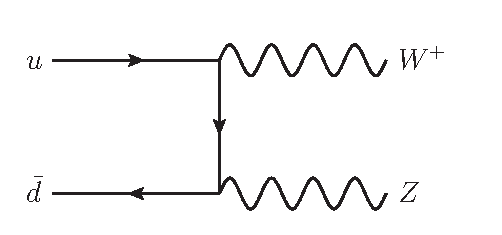
\includegraphics{figures/fd/diboson_tchannel}}
	}
	\subfloat[$WZ$] {
		\resizebox{0.4\textwidth}{!}{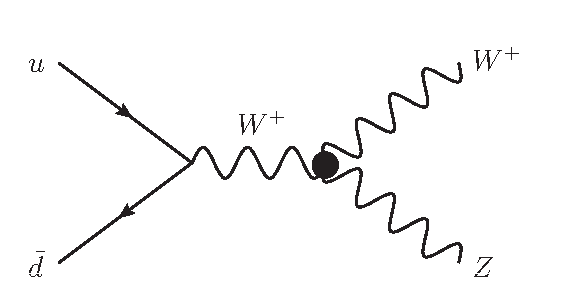
\includegraphics{figures/fd/diboson_schannel}}
	} \\
	\subfloat[$t\bar{t}+W$] {
		\resizebox{0.4\textwidth}{!}{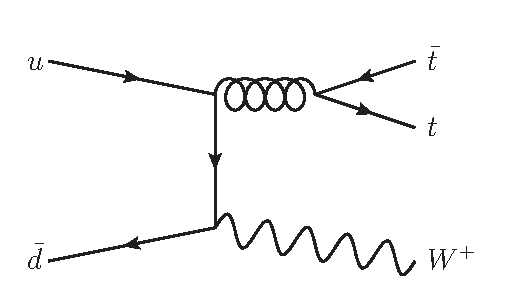
\includegraphics{figures/fd/ttW}}
	}
	\subfloat[$t\bar{t}+Z$] {
		\resizebox{0.4\textwidth}{!}{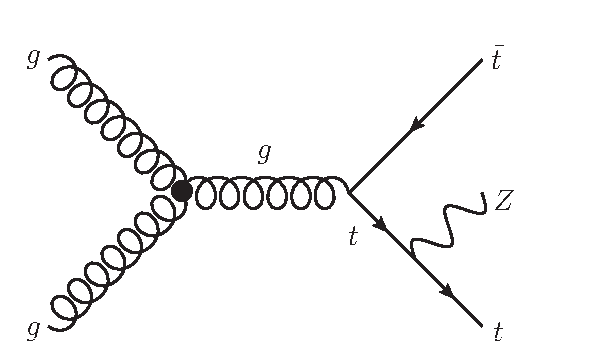
\includegraphics{figures/fd/ttV_gg_schannelg}}
	} \\
	\subfloat[$VVV^{*}$] {
		\resizebox{0.4\textwidth}{!}{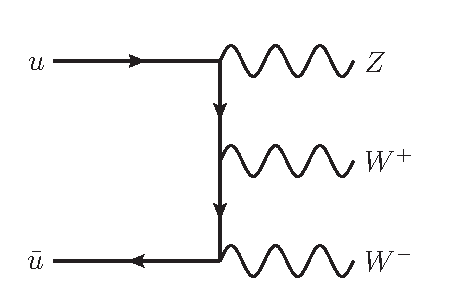
\includegraphics{figures/fd/VVV_qq}}
	}
	\subfloat[$VVV^{*}$] {
		\resizebox{0.4\textwidth}{!}{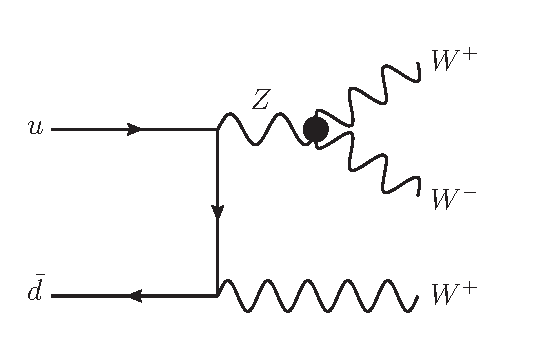
\includegraphics{figures/fd/VVV_TGC}}
	} \\
	\caption{Example tree-level Feynman diagrams of Standard Model processes leading to trilepton final states.}
	\label{fig:multilepton-feynman-diagrams}
\end{figure}


\section{Prompt Backgrounds}\label{sec:prompt-backgrounds}
The prompt backgrounds are estimated using Monte Carlo simulation. The hard-scattering processes are modeled by dedicated event generators, possibly including the emission of additional partons. Additional QCD radiation is modeled using a parton shower. The detector response to the simulated events is simulated with the ATLAS simulation framework~\cite{TheATLASCollaboration:2010et} using the \geant\ toolkit~\cite{Agostinelli:2002hh}. Pileup is included by overlaying simulated minimum-bias interactions from \pythia~\cite{pythia6} on the hard scattering event. Simulated events are assigned weights to reproduce the observed pileup distributions in data, and also to account for small differences in the trigger, reconstruction, and identification efficiencies between simulation and data. 

The details of the modeling of each sample are described below. The generator, parton shower, PDF set, underlying event tune, and accuracy of theoretical cross section for samples are summarized in table~\ref{table:mc-generators}.

\begin{itemize}
	\item \sherpa~\cite{sherpa} is used to model $WW$, $WZ$, and $ZZ$ production. Both bosons in the events decay leptonically. Up to three jets are included in the matrix element. An important feature of \sherpa\ is that it accurately models the $W+\gamma^{*}$ and $Z+\gamma^{*}$ contributions down to very low $\gamma^{*}$ masses; for electron decays, a cut of $m(ee)>100 \MeV$ is applied, while for muon and tau decays, \sherpa\ naturally cuts off the divergence. To increase the statistics in the phase space relevant for this analysis, the $WZ$ samples requires at least two leptons have $\pt>5 \GeV$. Finally, the $WZ$ sample also treats the $b$ and $c$ quarks as massive, which improves the modeling of heavy flavor jets at the cost of increased computation time. 
	\item \sherpa\ is also used to model $Z+\gamma$ production, where the photon converts asymmetrically in the detector and is reconstructed as an electron. The events are reweighted to account for observed mismodeling in the conversion rate, described in section~\ref{sec:conversion-reweighting}.
	\item $\ttbarV$ production is modeled with \madgraph~\cite{madgraph}, with \pythia\ for the parton shower.
	\item $WWW^{(*)}$, $ZWW^{(*)}$, and $ZZZ^{(*)}$ are modeled using \madgraph, with \pythia\ for the parton shower. Their contributions to all the signal regions are negligible.
\end{itemize}

\begin{table}
  \centering
  \scriptsize
  \begin{tabular}{|c|c|c|c|c|c|}
    \hline
    Process & Generator & Parton shower and hadr. & PDF set & UE tune & Cross section \\
    \hline
    $WZ$ & \sherpa~1.4.3 & \sherpa & CT10~\cite{ct10} & \sherpa 	&	NLO\\
    $ZZ$ & \sherpa~1.4.5 & \sherpa & CT10 & \sherpa 	&	NLO\\
    $\ttbar+W/Z$ & \madgraph\ 5.1.3.33  & \pythia\ 6.426   & CTEQ6L1~\cite{ct6l1} & AUET2B~\cite{AUET2B} 	&	NLO\\
    $VVV^{(*)}$ & \madgraph\ 5.1.3.33 & \pythia\ 6.426 & {CTEQ6L1}  & AUET2B 	& 	LO	\\
    $Z+\gamma$ & \sherpa  & \sherpa & CT10 & \sherpa 	&	LO 	\\
    \hline
  \end{tabular}
  \caption{Summary of the \textcolor{black}{primary} background MC samples used in this analysis. The generator, parton shower and hadronization, PDF, underlying event tune, and the order of the cross section calculation are shown for each sample.}
  \label{table:mc-generators}
\end{table}


\section{Reducible Backgrounds}\label{sec:reducible-backgrounds}
The reducible backgrounds encompass a variety of processes in which a reconstructed lepton arises due to something away from the ``hard scatter'' interaction. The backgrounds are estimated using simulation or a data-driven technique, depending on the source. The contribution from $Z+\gamma$, where the photon converts asymmetrically and is reconstructed as an electron, is estimated from Monte Carlo, with scale factors applied to account for an observed overestimation in the photon-to-electron conversion rate (see section~\ref{sec:photon-conversions}). Other reducible contributions, such as $W/Z+$jets or $t\overline{t}$ where a jet fakes an electron or decays semileptonically, are estimated in a data-driven manner using the \emph{fake factor} method. 


\subsection{Fake Factor Method}\label{sec:fake-factor-method}
The fake factor method estimates the reducible backgrounds in each signal region by characterizing the fake or non-prompt leptons in terms of quantities sensitive to the fake process, such as isolation, impact parameter, or particle identification cuts. Two orthogonal sets of leptons are defined: \emph{numerator} leptons ($N$) satisfy the nominal signal lepton selection criteria, while \emph{denominator} leptons ($D$) satisfy most of the nominal selection criteria, except with inverted requirements on quantities sensitive to the fake process. The reducible background is estimated in a data-driven way from a control region consisting of events with a mix of numerator and denominator leptons, together with a parametrization of the relationship between numerators and denominators. 

The relationship between numerator and denominator objects is called the \emph{fake factor}, $f$, defined as the ratio of the number of fake leptons satisfying the numerator criteria to those satisfying the denominator criteria. The fake factor is measured in a control region enriched in fake leptons. The success of the method depends largely on the extrapolation of the $f$ from the measurement control region to the signal regions. To capture the dependence on the event kinematics, $f$ can be measured as a function of various lepton or event variables; in this dissertation, the fake factors are all measured in bins of lepton $\pt$ and $\eta$. 

Once $f$ has been measured, the reducible background is determined as follows. In signal events with three or more leptons, any subset of the leptons could be real or fake. For example, an event might contain two real leptons from a Drell-Yan process plus a fake third lepton. Such an event is labeled $\RRF$, indicating the ``truth'' classification of the three leptons as either real ($R$) or fake ($F$) (the ordering of the letters corresponds to some canonical order of the leptons, such as $\pt$ ordering). On the other hand, if an event contained, say, $W\rightarrow l\nu$ plus two fake leptons, the event would be labeled $\RFF$ (or $\FRF$ or $\FFR$). 

The quantity we desire to determine is the number of events containing three real leptons, $n_{\RRR}$. The quantity actually measured in a signal region is the number of events containing three numerator objects, $n_{\NNN}$. Any of these numerators could be real or fake, so the sample can be decomposed as:

\begin{align}
	n_{\NNN} & = n_{\RRR} + n_{\RRF} + n_{\RFR} + n_{\RFF} +\\
	&  \hspace{0.5in} + n_{\FRR} + n_{\FRF} + n_{\FFR} + n_{\FFF}
\end{align}

The reducible background prediction is $n_{\NNN}-n_{\RRR}$, the number of signal events where at least one lepton is fake. To determine the other terms, we use events with one or more denominator leptons. For example, consider $\DNN$ events, where the first lepton is a denominator and the remaining leptons are numerators. Assuming that the denominator lepton is always a fake lepton, the number of $\DNN$ events, each weighted by the fake factor $f$ corresponding to the denominator lepton (represented schematically by $n_{\DNN}f_{1}$), equals the number of $\NNN$ events where the first lepton is fake:

\begin{align}
	n_{\DNN} f_{1} &= n_{\FRR} + n_{\FRF} + n_{\FFR} + n_{\FFF}.
\end{align}

Similarly, the remaining permutations of numerators and denominators yield:

\begin{align}
	n_{\NDN} f_{2} &= n_{\RFR} + n_{\RFF} + n_{\FFR} + n_{\FFF} \\
	n_{\NND} f_{3} &= n_{\RRF} + n_{\RFF} + n_{\FRF} + n_{\FFF} \\
	n_{\DDN} f_{1}f_{2} &= n_{\FFR} + n_{\FFF} \\
	n_{\DND} f_{1}f_{3} &= n_{\FRF} + n_{\FFF} \\
	n_{\NDD} f_{2}f_{3} &= n_{\RFF} + n_{\FFF} \\
	n_{\DDD} f_{1}f_{2}f_{3} &= n_{\FFF}
\end{align}

These equations contain eight equations and eight unknowns, so the system can be solved for the reducible background prediction:
\begin{align} \label{eq:fake-factor-master-formula}
	\NNN - \RRR &= \left( \NND f_{3} + \NDN f_{2}  + \DNN f_{1}\right)  \\
		 & \hspace{0.5in} - \left( \NDD f_{2}f_{3} + \DND f_{1}f_{3} + \DDN f_{1}f_{2}\right) \\
		 & \hspace{0.5in} + \DDD f_{1}f_{2}f_{3}
\end{align}

Note that throughout this method, we have assumed that the leptons used for the measurement of $f$ and the denominator leptons in trilepton events are always fake leptons. In practice, real leptons contaminate both of these samples, and is accounted for using simulation, where the lepton can be classified as real or fake using the truth record of the event.

We now discuss the measurement of the fake factors $f$, separately for electrons, muons, and tau leptons.

\subsection{Electron Fake Factors}\label{sec:electron-fake-factors}
The background estimation for fake electrons targets the reducible contribution from two sources: semileptonic heavy flavor decays and misidentified light hadrons. The electron denominator objects are defined by inverting either the IsEM electron identification criteria~\footnote{The parameter space between medium++ and loose++, rather than tight++ and medium++, is used for two reasons. First, for the model-independent trilepton analysis (chapter~\ref{ch:model-independent-trilepton-search}), electrons passing medium++ and failing loose++ are used to define a validation region to test the fake factor method. Second, requiring the electrons to fail medium++ reduces the prompt contamination in the denominator sample.} or the track impact parameter cut (exclusive OR), as shown in table~\ref{table:electron-denominator-definition}; the electron must pass all the remaining cuts listed in table~\ref{table:electron-muon-selections}. Additionally, an inefficiency is observed for loose offline electrons with respect to the loose electron triggers. This is due to the lack of Gaussian sum filter (GSF) tracking~\cite{TheATLASCollaboration:2012vr} at the trigger level. The inefficiency is mitigated by imposing the \verb.tight++. requirement on the $\Delta\eta$ and $\Delta\phi$ between the electron track and associated calorimeter cluster, with the goal of cutting out electrons with large amounts of bremsstrahlung, whose tracks are not reconstructed by the non-GSF algorithm in the trigger. 


\begin{table}[h]
  \centering
  \begin{tabular}{ccc}
	\hline
	Criteria & Numerator & Denominator \\ \hline
	IsEM ID & \verb.tight++. & !\verb.medium++. \&\& \verb.loose++.  \\
	Impact Parameter Significance & $\frac{|d_0|}{\sigma_{d_0}} < 3$ & $3 < \frac{|d_0|}{\sigma_{d_0}} < 10$ \\
	\hline
  \end{tabular}
  \caption{Electron denominator definitions. The denominators are taken to be an exclusive OR combination of the two selection inversions. Additionally, denominator objects must pass the tight requirement on the $\Delta\eta$ and $\Delta\phi$ between the track and the cluster.}
  \label{table:electron-denominator-definition}
\end{table}

The fake factors are measured in a control sample of single-electron events, using the entire $20.3~\mbox{fb}^{-1}$ 2012 dataset. The triggers used to collect events are listed in table~\ref{table:electron-fake-factor-triggers}; photon triggers are used where available ($\pt>24~\mbox{GeV}$), and loose electron triggers are used otherwise ($15~\mbox{GeV}<\pt<24~\mbox{GeV}$). 

\begin{table}[h]
  \centering
  \begin{tabular}{ccc}
  \hline
	$p_T$ range (GeV) & Trigger & Average 2012 Prescale \\
	\hline
	15-17 & EF\_e5\_loose0 & 56080.5\\
	17-24 & EF\_e15vh\_loose0 & 1549.7\\
	24-45 & EF\_g20\_loose & 4412.6\\
	45-65 & EF\_g40\_loose & 348.3\\
	65-85 & EF\_g60\_loose & 80.9\\
	85-105 & EF\_g80\_loose & 28.5\\
	105-125 & EF\_g100\_loose & 13.0\\
	125-210 & EF\_g120\_loose & 1.0\\
	$>$210 & EF\_g200\_etcut & 1.0\\ \hline
  \end{tabular}
  \caption{Trigger used to collect electron numerator and denominator objects.}
  \label{table:electron-fake-factor-triggers}
\end{table}

Events are required to have $m_{\mathrm{T}}<40~\mbox{GeV}$ and $\Etmiss<40~\mbox{GeV}$ to suppress contamination from single-$W$ production, where $m_{\mathrm{T}}$ is the transverse mass of the electron and missing transverse energy in the event. The events are also required to have exactly one electron, numerator or denominator, in order to suppress prompt contamination from $Z\rightarrow ll$ events. The electrons are required to be trigger-matched to the trigger used to collect the event in the relevant $\pt$ range. The residual prompt contamination, comprised mostly of $W$ and $Z$ events with smaller contributions from Drell-Yan, $t\overline{t}$ and single-$t$, is subtracted using Monte Carlo. The numerator and denominator event yields, as well as the predicted prompt contamination, are shown in figure~\ref{fig:el-ff-data-prompt-subtractions}. The prompt contamination consists primarily of $W$ and $Z$ events. The relative size of the prompt contamination is quite large for numerator objects, reaching up to $\sim60\%$ for $\pt\sim 50~\mbox{GeV}$, despite the cuts intended to reduce the $W$ contribution. The fake factors are binned two-dimensionally in $\pt$ and $\eta$, shown in figure~\ref{fig:electron-fake-factor-values}. The $\pt$ dependence of the fake factors is shown in figure~\ref{fig:electron-fake-factors-1D-pt}, for the inclusive sample (left) and for various $|\eta|$ ranges (right).

\begin{figure}
  \centering
  % TODO: Make the legends consistent between the plots. Currently the legend entries are sorted by histogram integral, independently for the left and right plots.
  \subfloat[Numerators, log scale] {
	\resizebox{3in}{!}{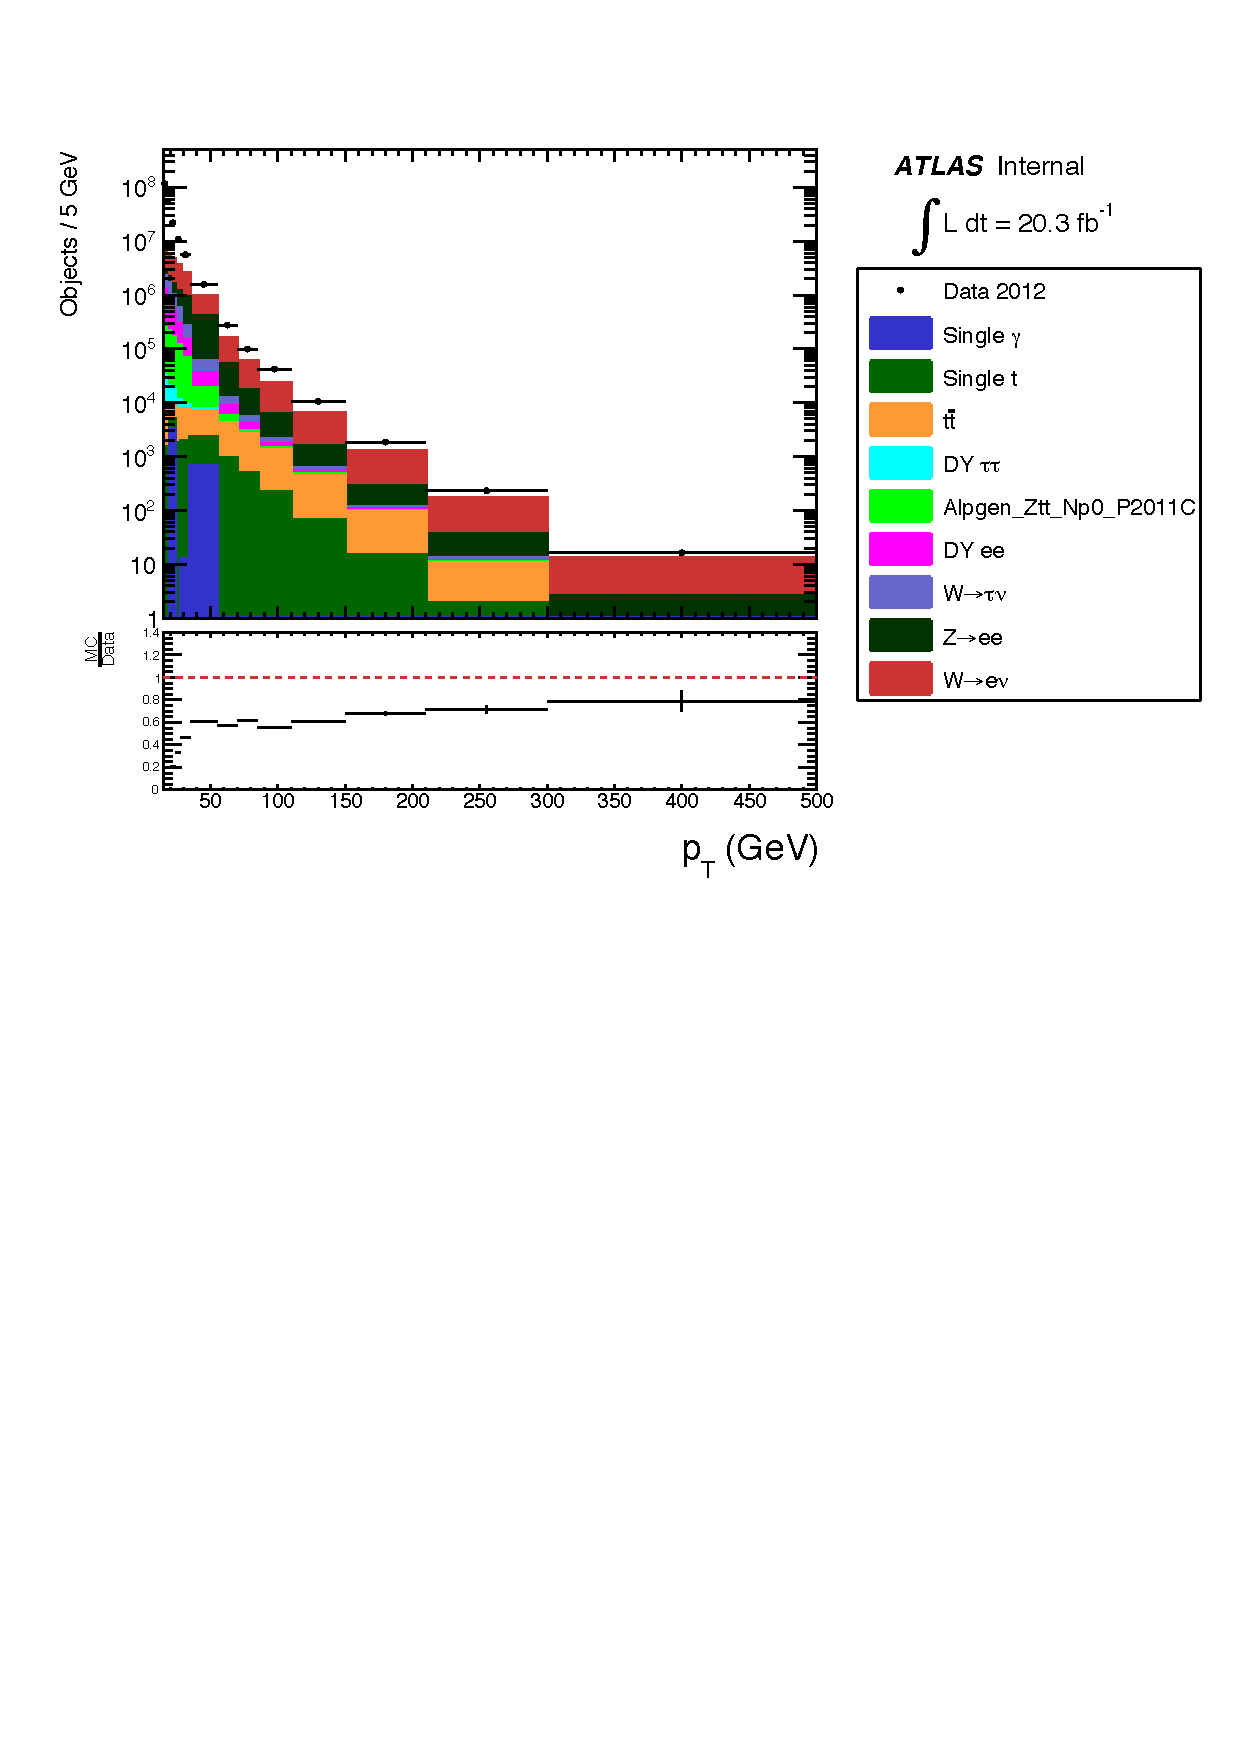
\includegraphics{figures/backgrounds/c_ElectronNumerator_pt_log}}
	\label{f:numlogscale}
  }
  \subfloat[Denominators, log scale] {
	\resizebox{3in}{!}{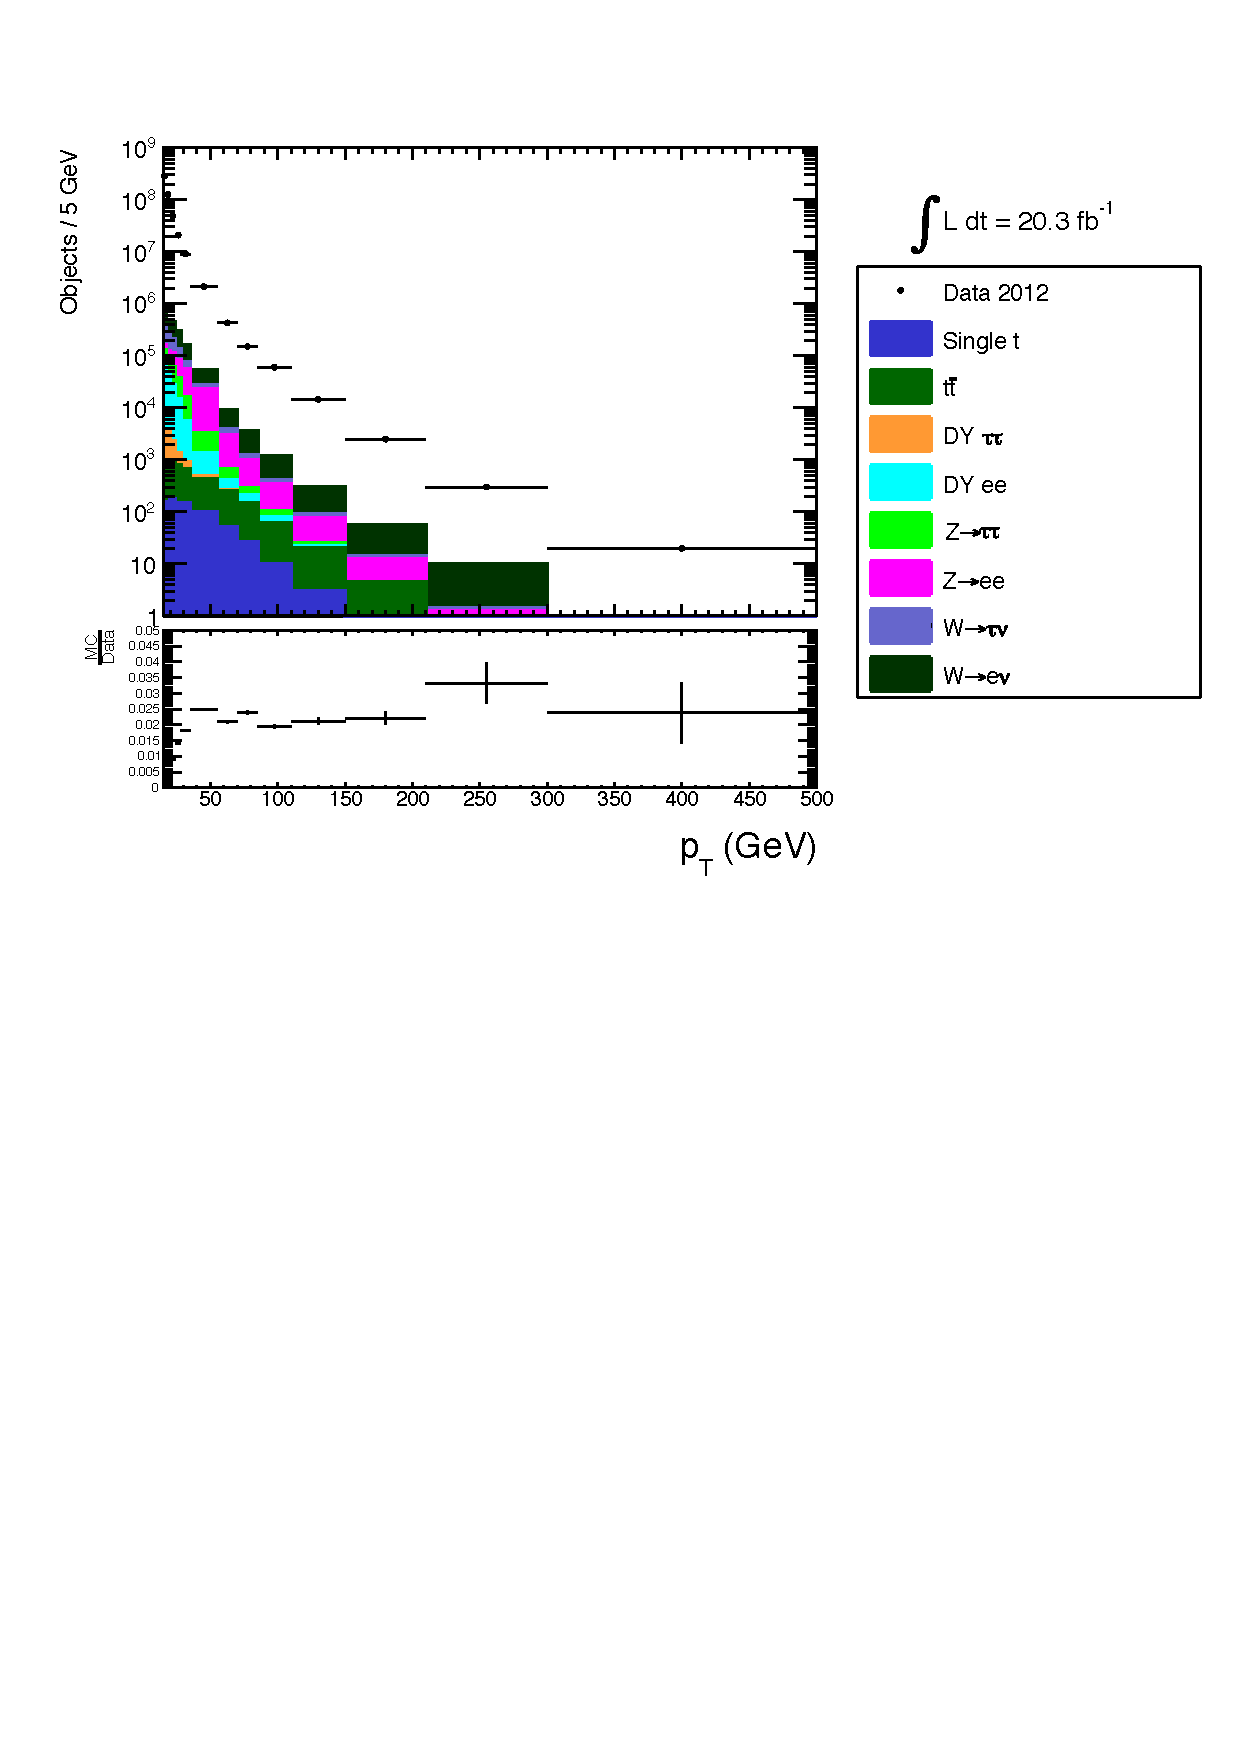
\includegraphics{figures/backgrounds/c_ElectronDenominatorCombined_pt_log}}
	\label{f:denlogscale}
  } \\
  \subfloat[Numerators, linear scale] {
	\resizebox{3in}{!}{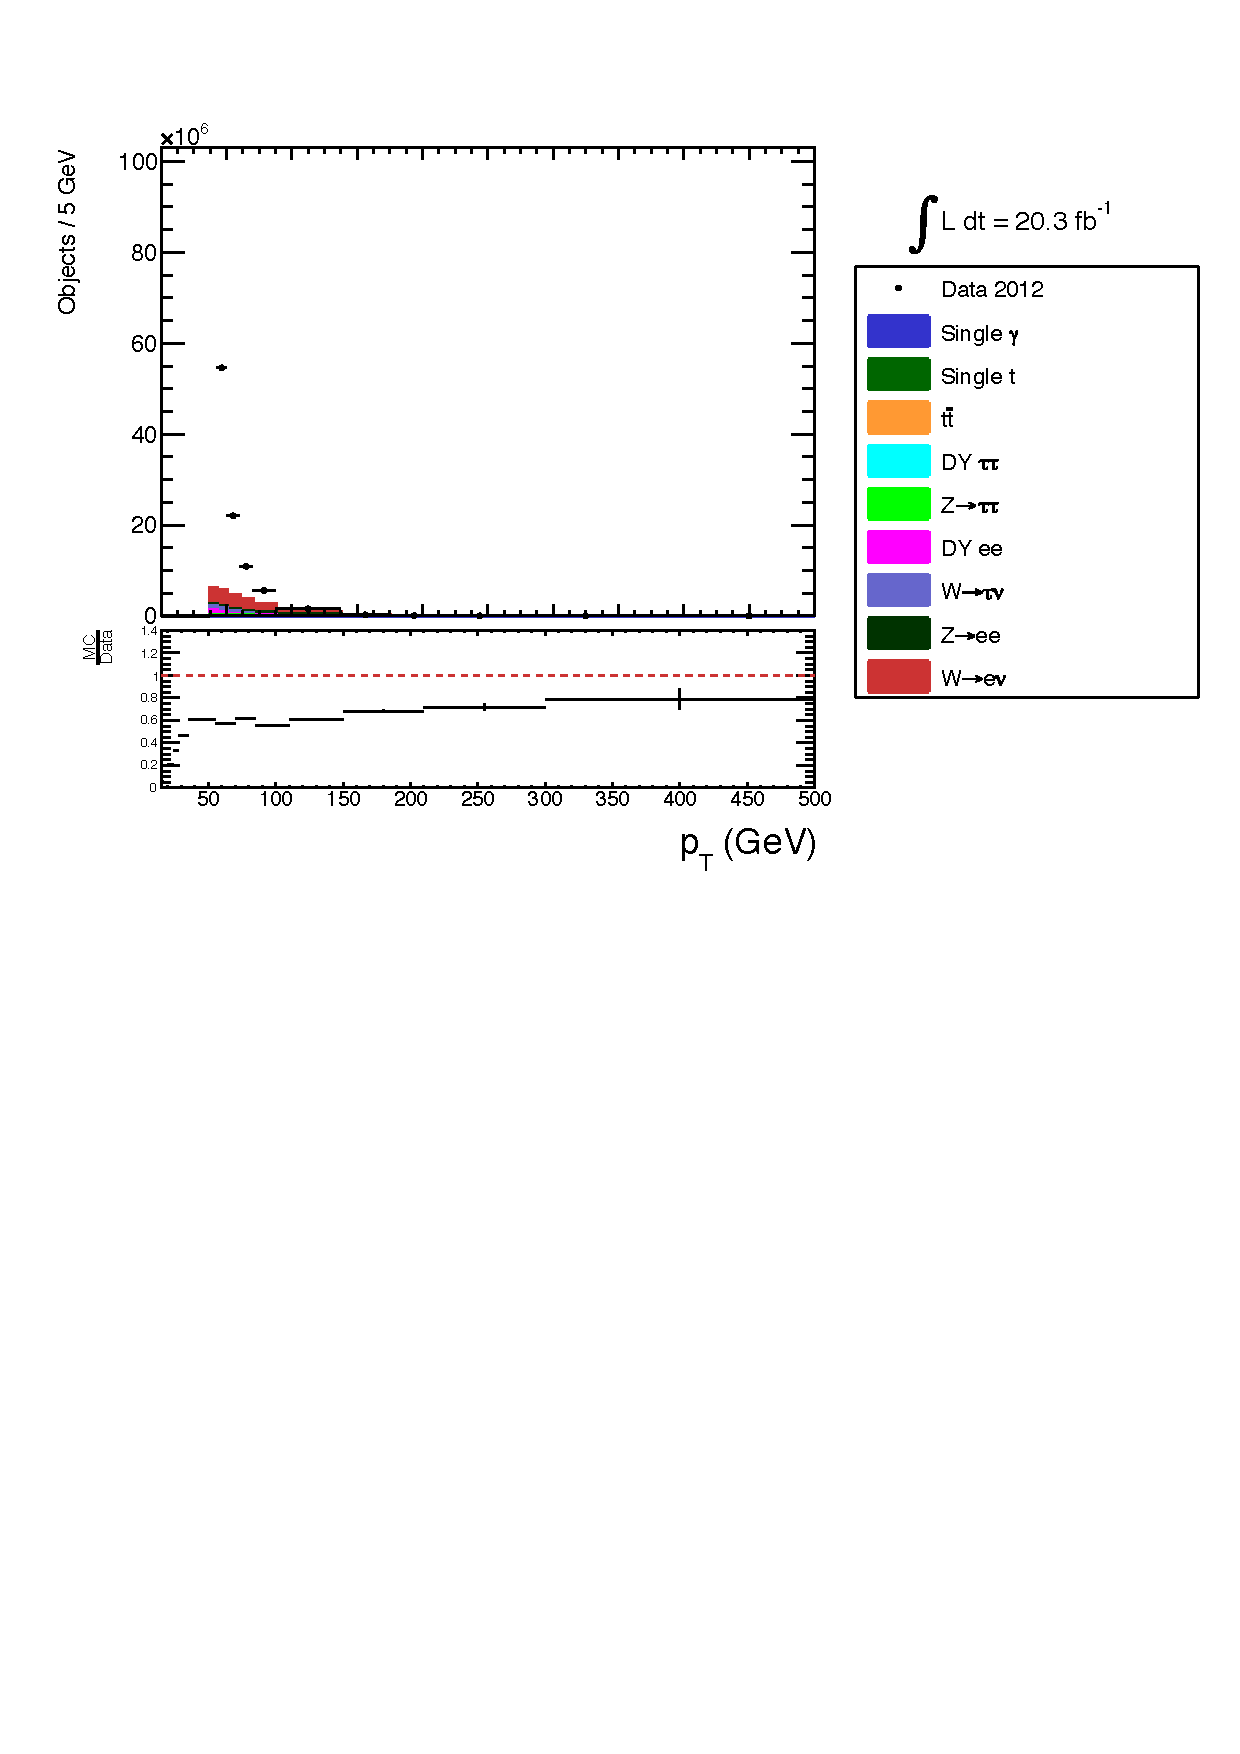
\includegraphics{figures/backgrounds/c_ElectronNumerator_pt_linear}}
	\label{f:numlinscale}
  }
  \subfloat[Denominators, linear scale] {
	\resizebox{3in}{!}{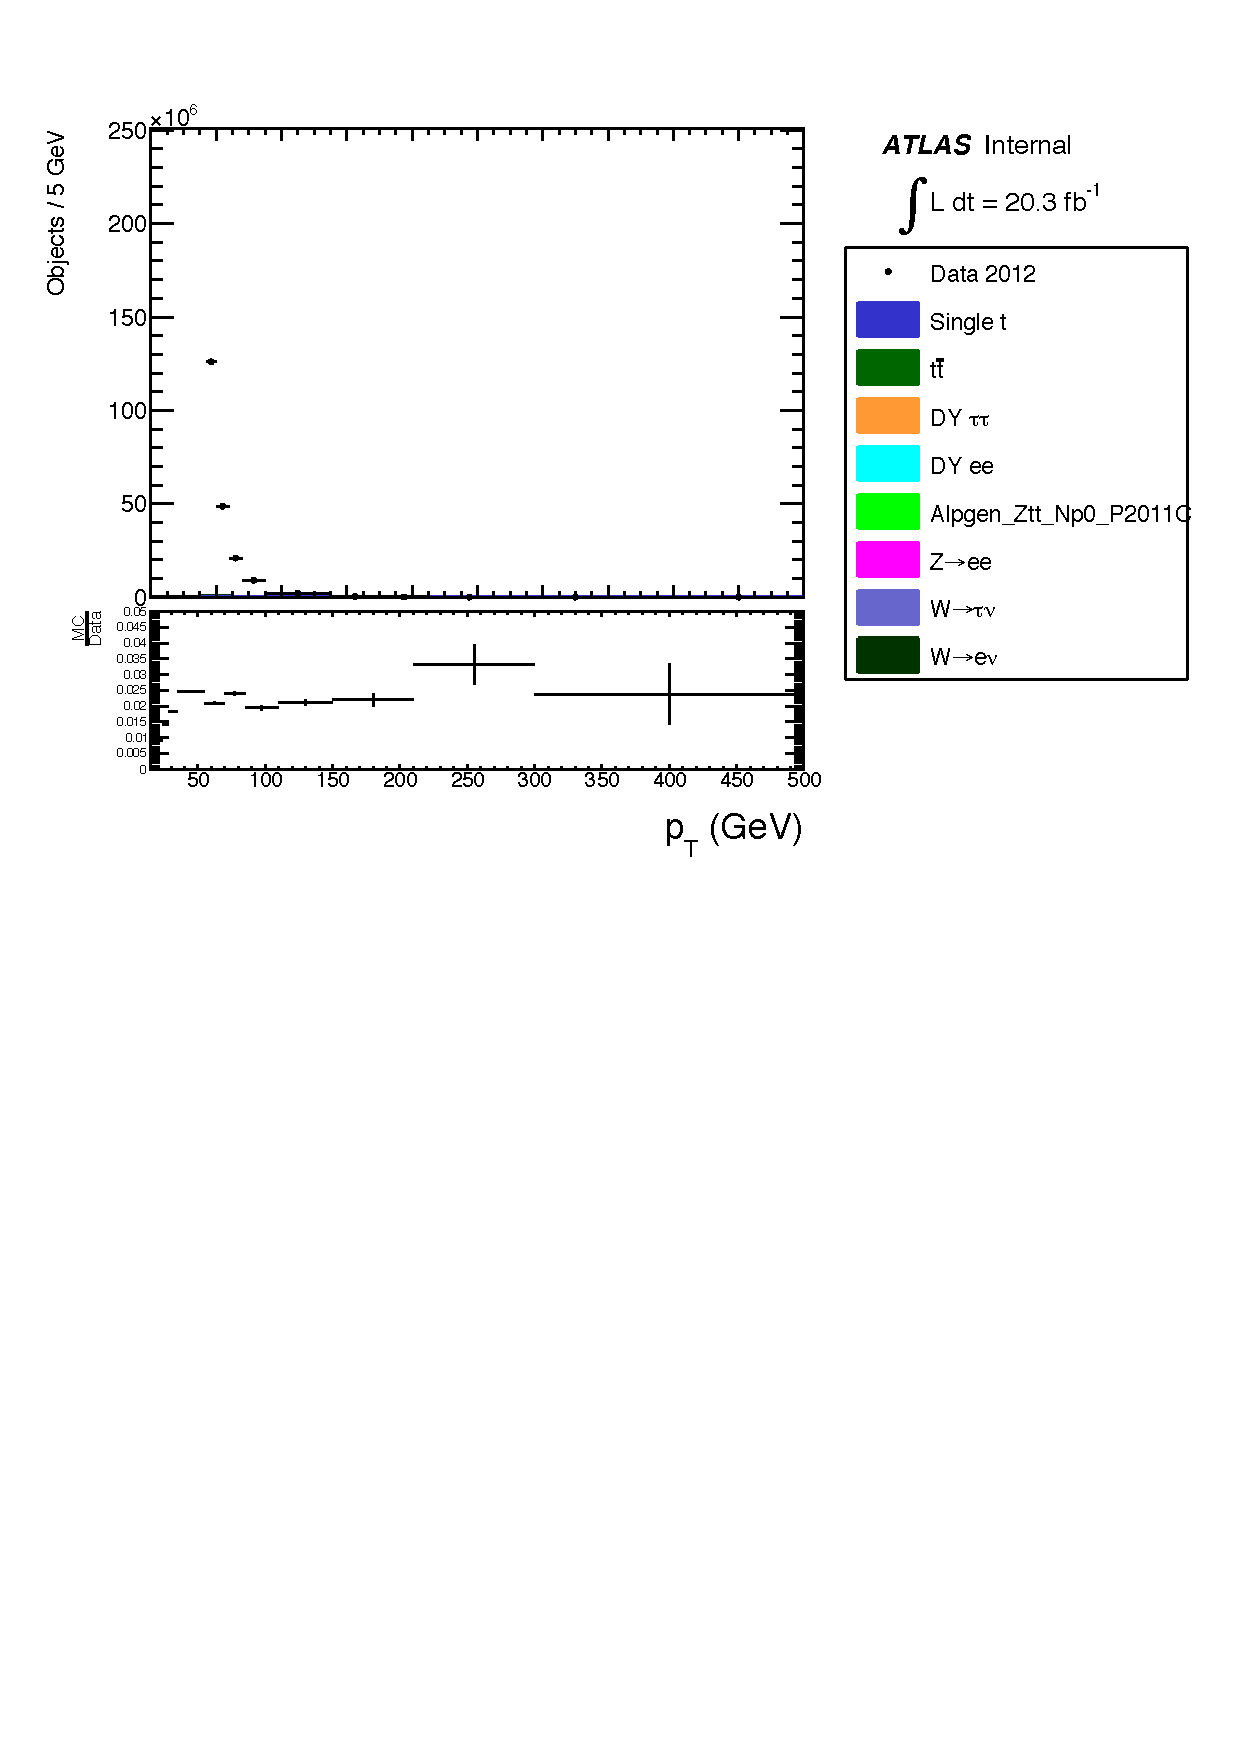
\includegraphics{figures/backgrounds/c_ElectronDenominatorCombined_pt_linear}}
	\label{f:denlinscale}
  } \\
  \caption{Numerator and denominator electron object counts. The data sample consists of all single-electron events in the 2012 dataset, with cuts to reduce prompt contamination as described in the text. The markers represent object counts from 2012 data, and the colored histograms indicate the prompt subtractions estimated from Monte Carlo.}
  \label{fig:el-ff-data-prompt-subtractions}
\end{figure}

\begin{figure}[h]
  \centering
  \subfloat[Central values] {
	\resizebox{3in}{!}{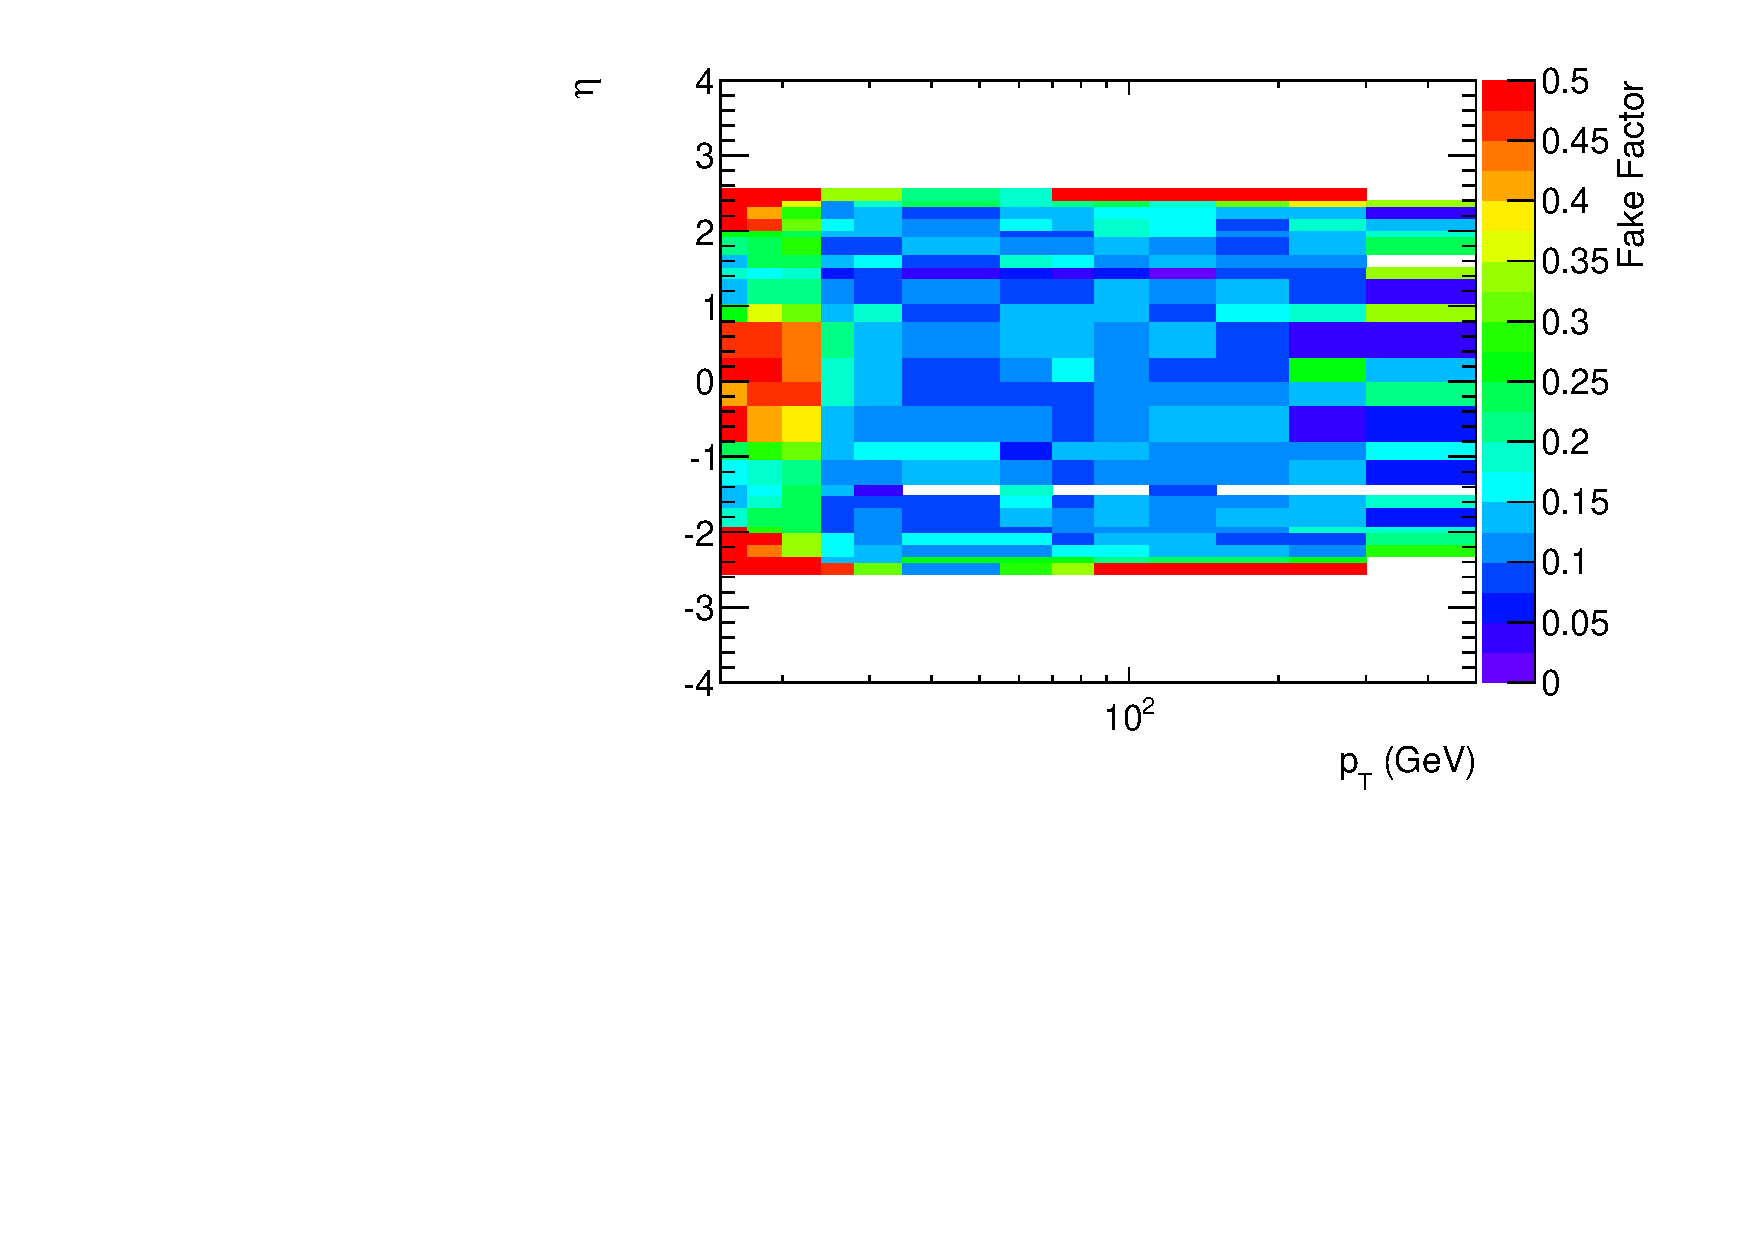
\includegraphics{figures/backgrounds/c_FinalFF_2D}}
  }
  \subfloat[Statistical uncertainty over value] {
	\resizebox{3in}{!}{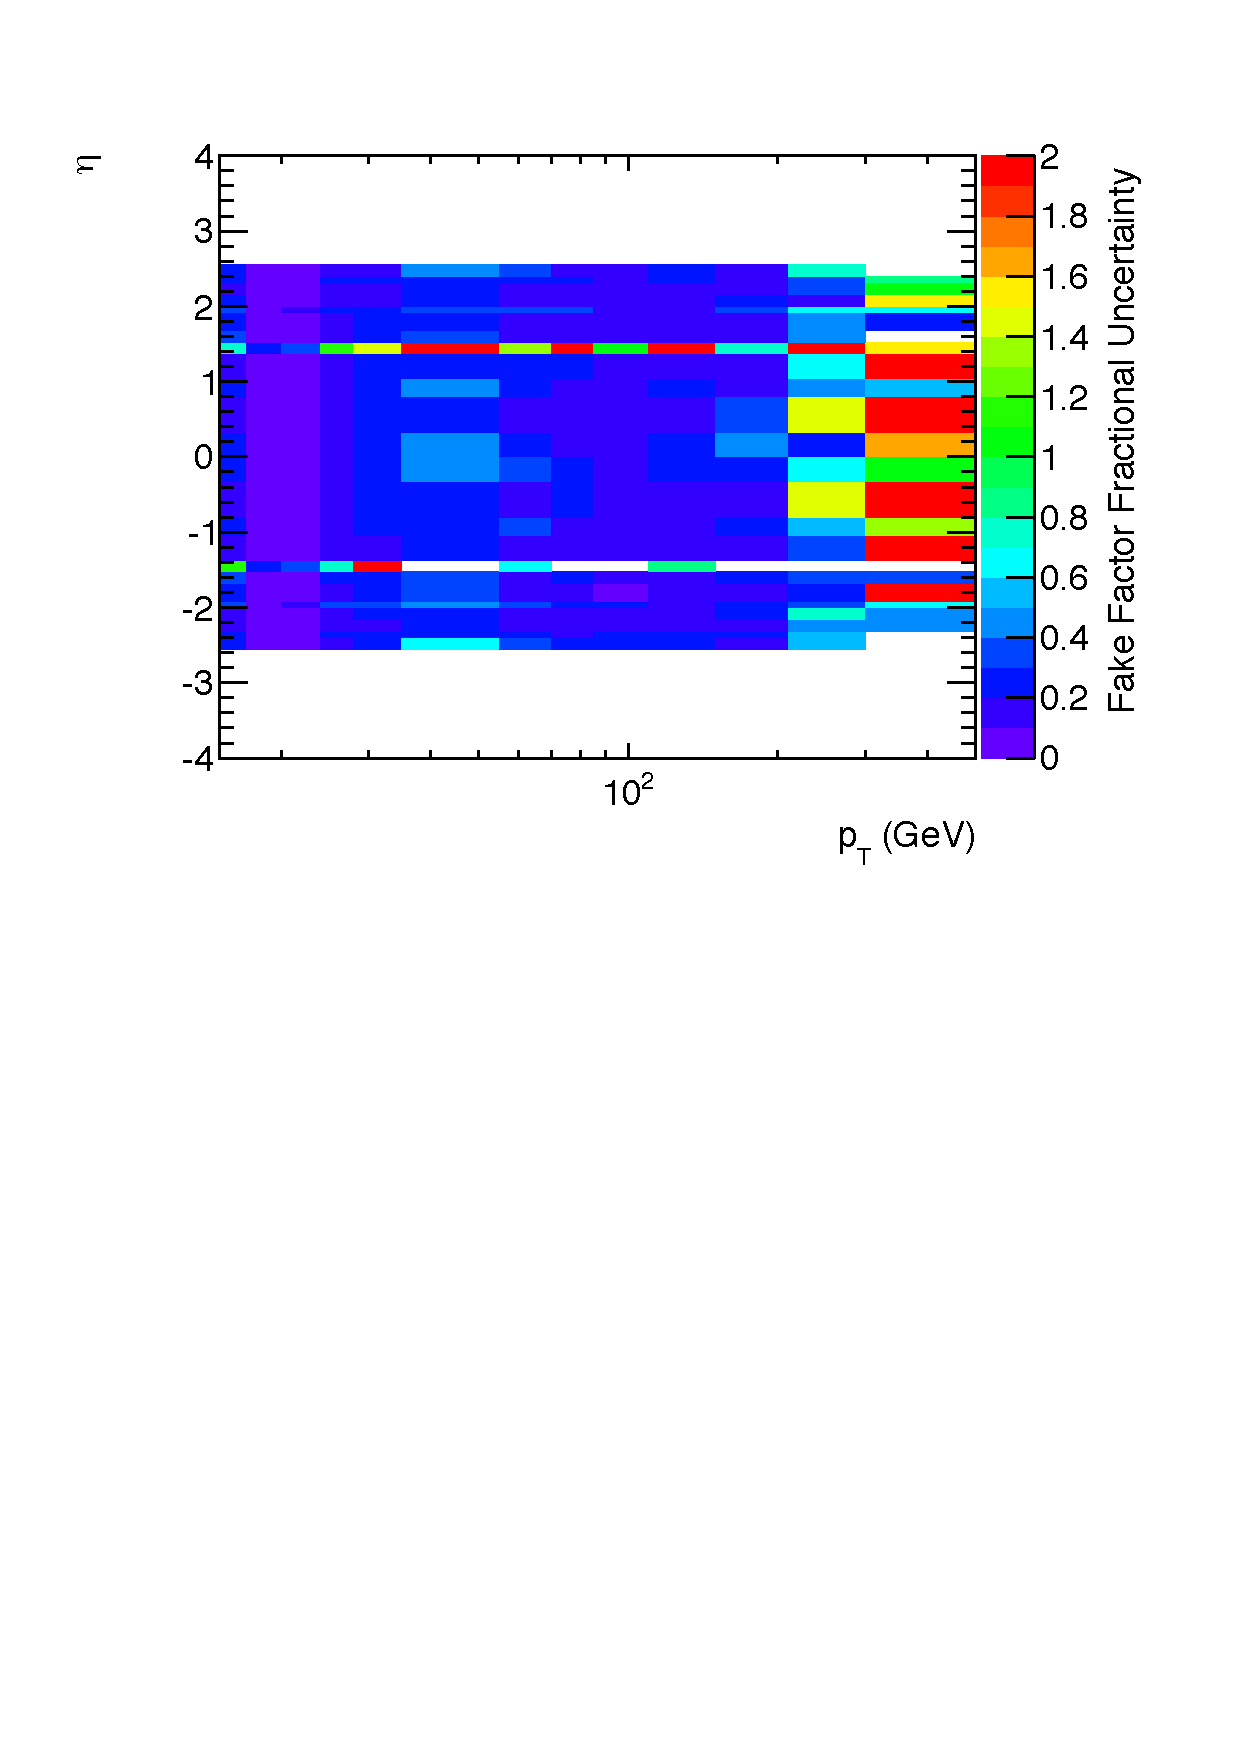
\includegraphics{figures/backgrounds/c_FinalFF_2D_ErrorOverValue_corr}}
  }
  \caption{Electron fake factors parametrized in $p_T$ and $\eta$.}
  \label{fig:electron-fake-factor-values}
\end{figure}

\begin{figure}[h] 
  \centering
  \subfloat[Average fake factor vs. $p_{\mathrm{T}}$] {
	\resizebox{3in}{!}{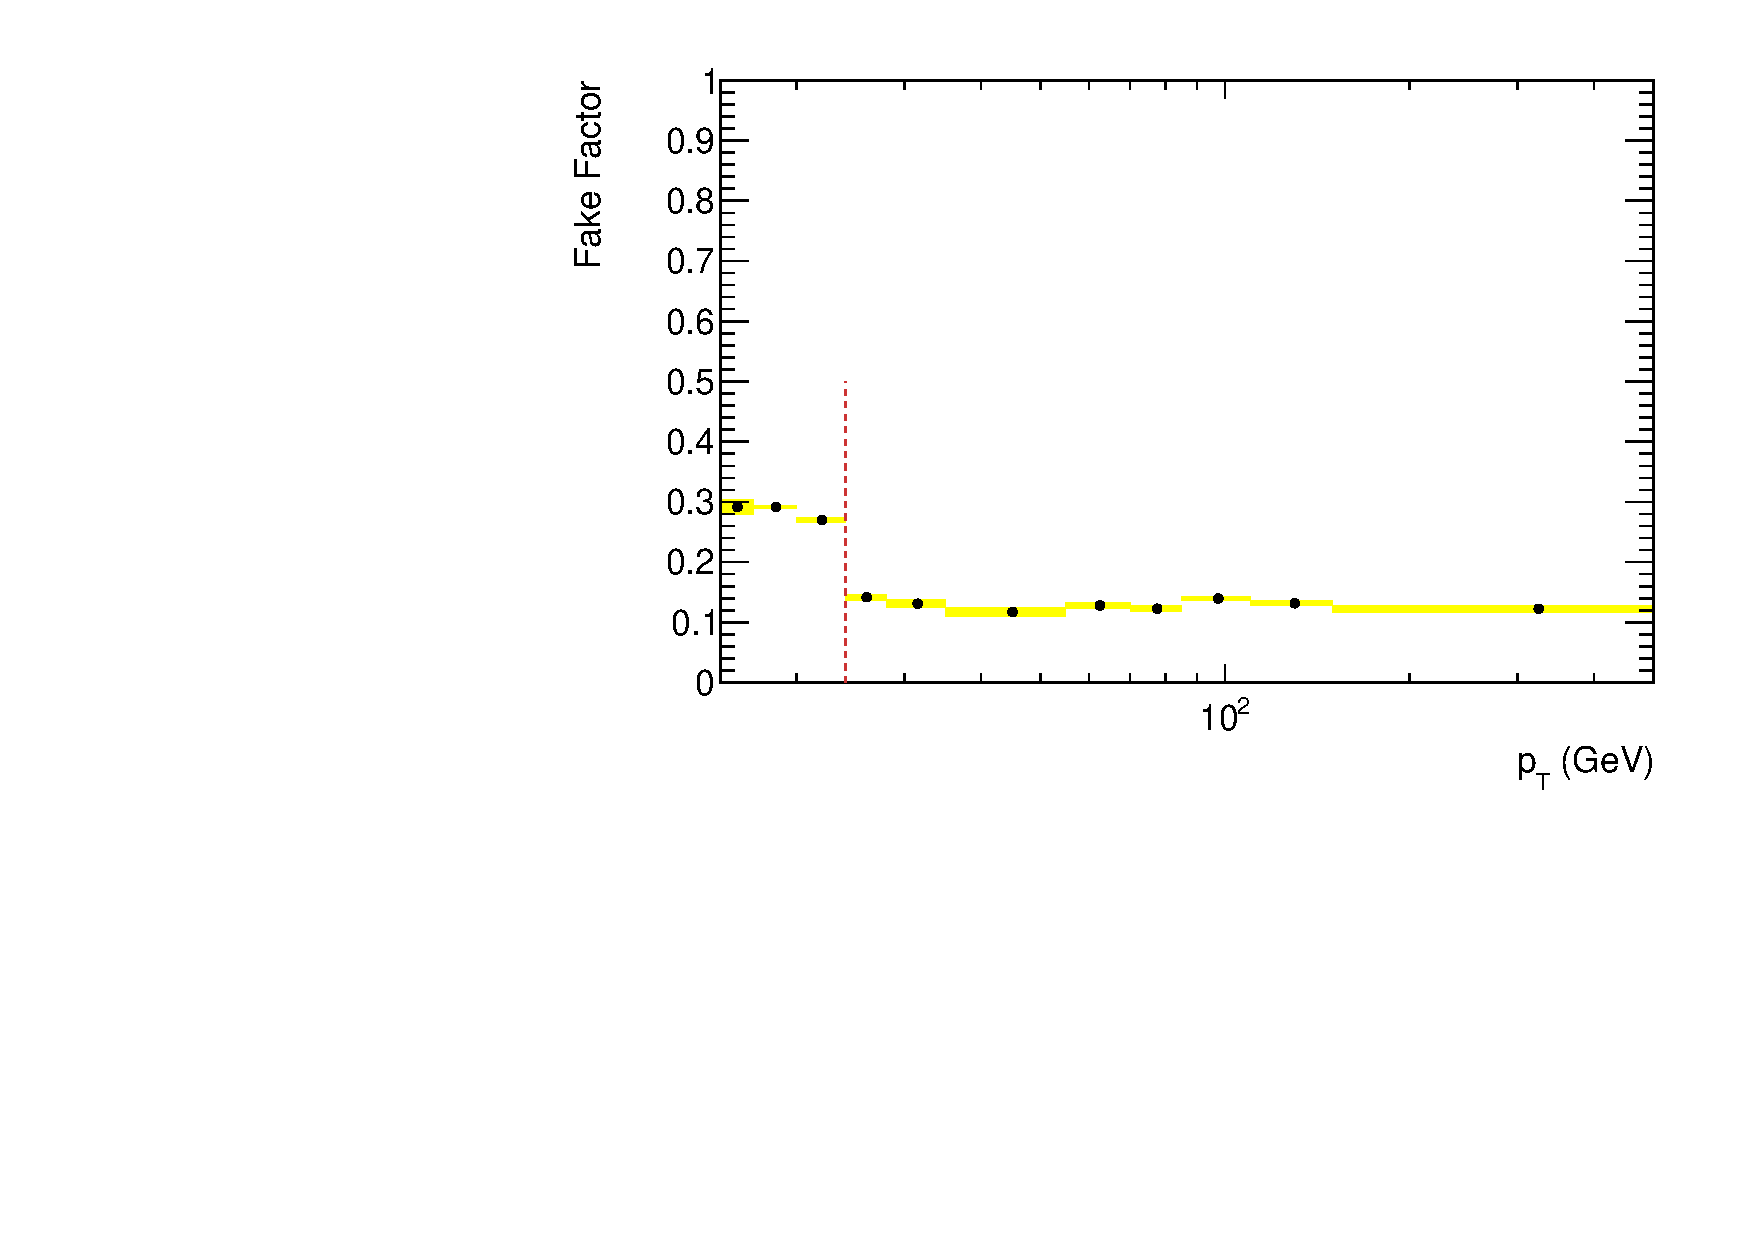
\includegraphics{figures/backgrounds/c_FinalFF_1D_pt}}
  }
  \subfloat[Fake factors vs. $p_{\mathrm{T}}$ for different value of electron $|\eta|$] {
	\resizebox{3in}{!}{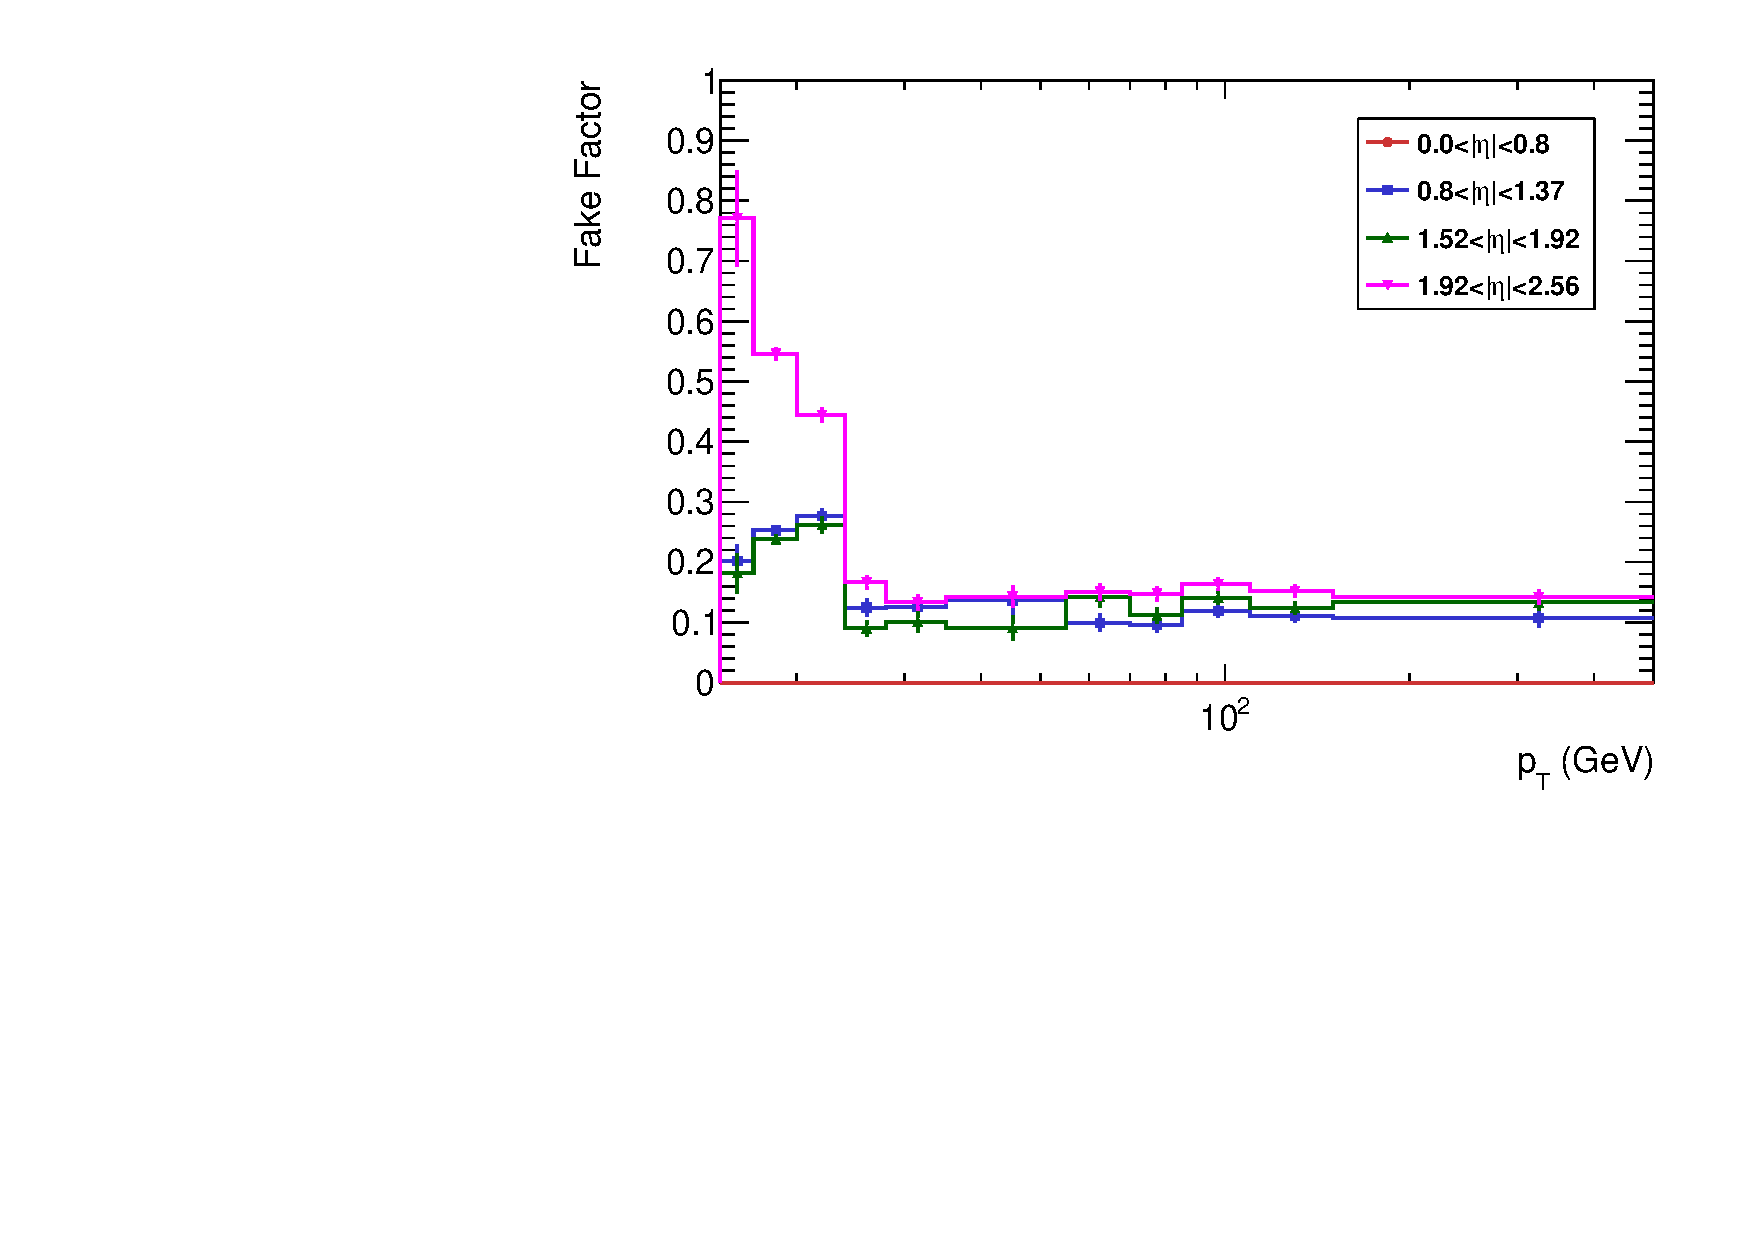
\includegraphics{figures/backgrounds/c_FinalFF_1D_etaslices}}
  }
  \caption{Electron fake factors projected in $p_{\mathrm{T}}$. The denominator requirements are different below and above $24~\GeV$, where the triggers switch from EF\_eXX to EF\_gXX; below, the additional requirements on $\Delta\eta_1$ and $\Delta\phi_2$ cause a large drop in the denominators, and a large increase in the fake factor values.}
  \label{fig:electron-fake-factors-1D-pt}
\end{figure}

To help clarify the origin of the structure in $\eta$ observed at low $\pt$, the numerator and denominator counts are also shown versus $\eta$ for $\pt<24~\mbox{GeV}$ in figure~\ref{fig:electron-num-den-eta-lowpt}. The numerator counts are relative flat versus $\eta$ in the central region, and grow for $|\eta|\gtrsim 2$. Conversely, the denominators exhibit a significant increase near the barrel-endcap overlap region, and also for $|\eta|\gtrsim 2$. 

\begin{figure}[h]
  \centering
  \resizebox{5in}{!}{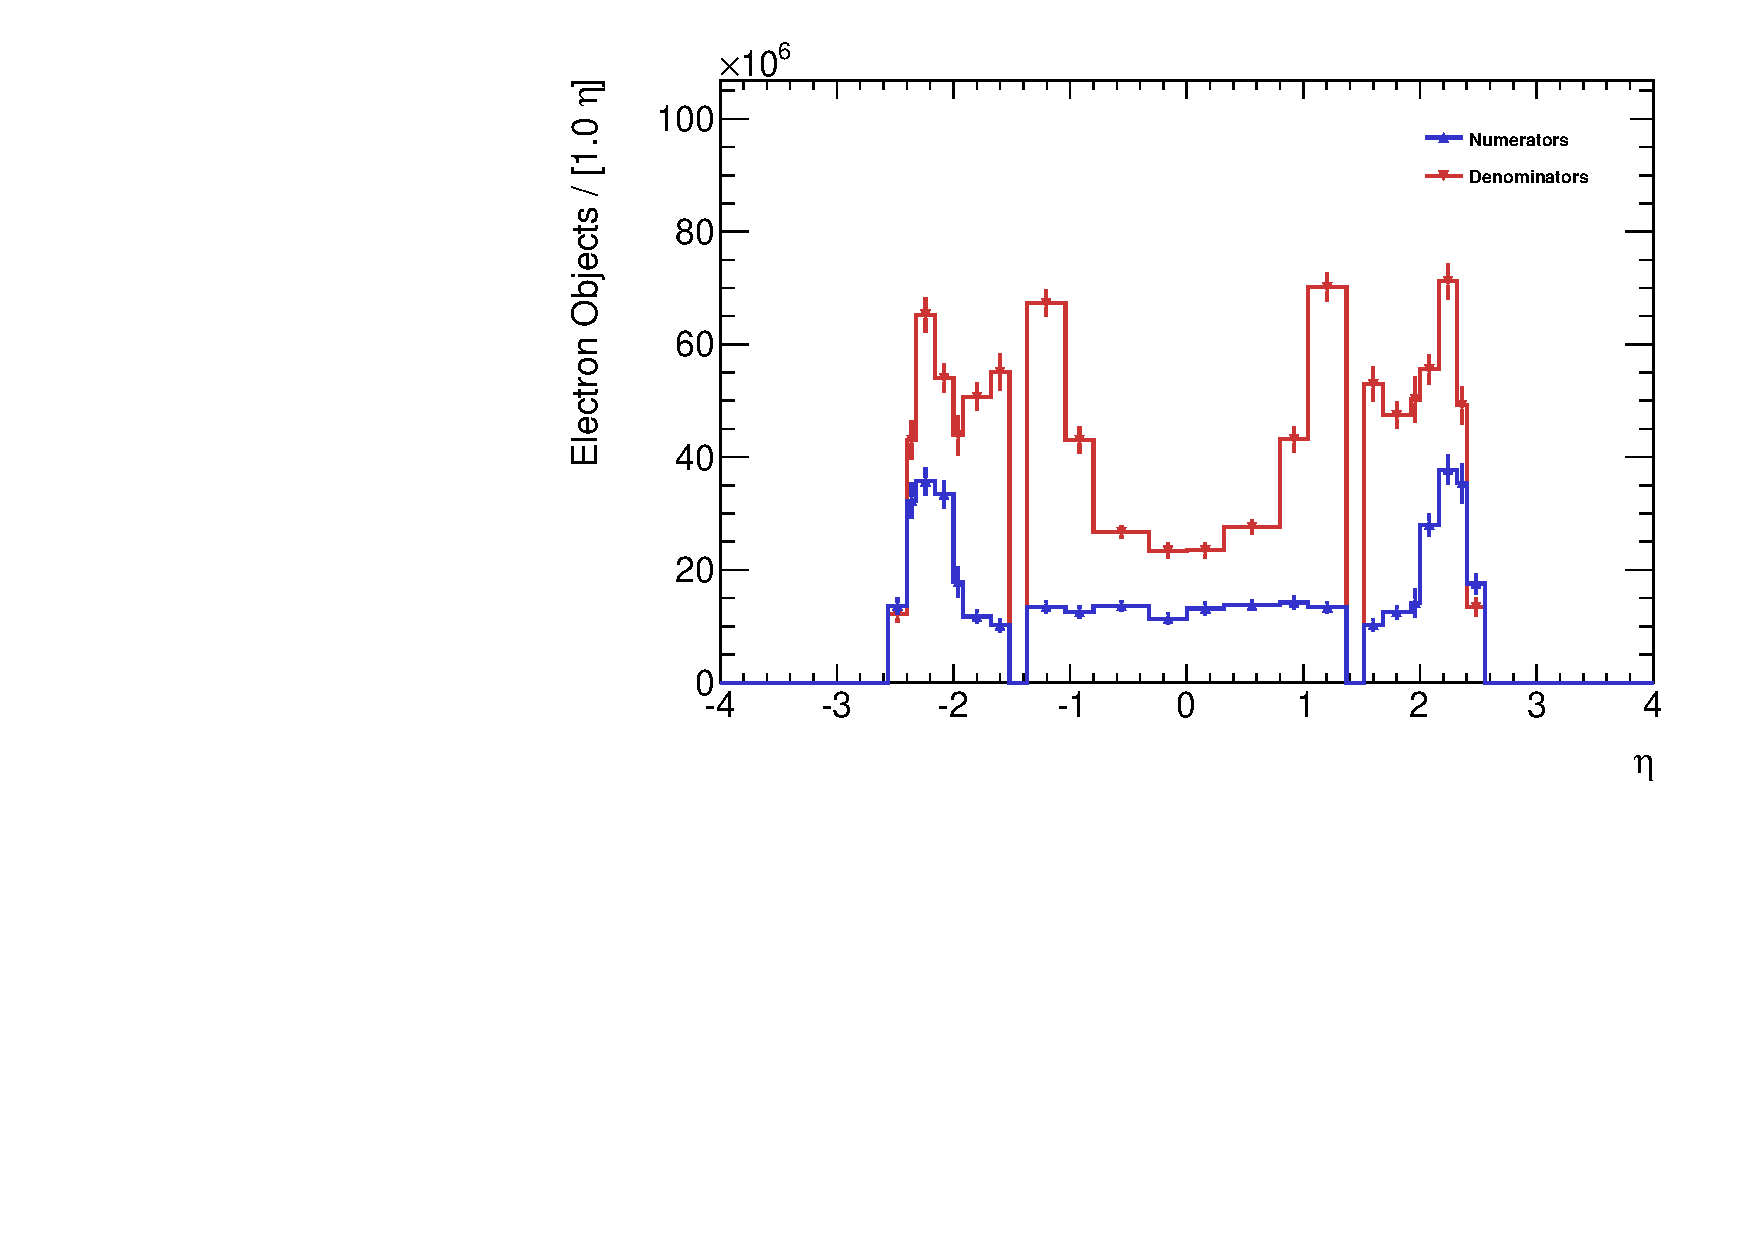
\includegraphics{figures/backgrounds/c_NumDen_lowPt_eta}}
  \caption{Electron numerator and denominator object counts versus $\eta$ for $\pt<24~\mbox{GeV}$.}
  \label{fig:electron-num-den-eta-lowpt}
\end{figure}


The following sources of systematic uncertainty are considered:
\begin{itemize}
  \item \textbf{Prompt subtraction}: The presence of real, prompt leptons from Standard Model processes in the sample used to measure the fake factors is accounted for using Monte Carlo simulation. Uncertainties on the simulated samples include luminosity; cross section uncertainties; and reconstruction, trigger, and identification efficiency scale factors. These lead to a maximum uncertainty of about $20\%$ where the prompt subtraction is largest. 
  \item \textbf{Trigger efficiency correction}: As mentioned previously, an inefficiency is observed in the loose electron triggers for offline \verb.loose++. electrons. This is due to the lack of GSF tracking in the trigger. For the fake factor derivation, this affects electrons in the range $15~\mbox{GeV}<\pt<24~\mbox{GeV}$, where photon triggers are not available. Imposing the \verb.tight++. cut on the track-cluster matching (the $\Delta \eta$ and $\Delta \phi$ between the electron track and calorimeter cluster) mitigates most, but not all, of the inefficiency, by cutting out electrons with large amounts of bremsstrahlung whose track are not reconstructed in the trigger. Based on a comparison of loose electron and photon triggers in the range $24~\mbox{GeV}<\pt<85~\mbox{GeV}$, a correction of about $8\%$ is applied to loose electron-triggererd events, and the same value is taken as systematic uncertainty.
  \item \textbf{Extrapolation to signal region}: Two systematic uncertainties are assigned to account for bias due to the extrapolation of fake factors from the control region to the signal region. First, the cuts on $m_{\mathrm{T}}$ and $\Etmiss$ are varied from $<40~\mbox{GeV}$ to $<25~\mbox{GeV}$ and $<55~\mbox{GeV}$. A $\pt$-dependent systematic uncertainty of up to $15\%$ is assigned. Second, Monte Carlo-based truth studies indicate that the fake factor values are quite different for heavy- and light-flavor jets, so a difference in heavy flavor fraction between the control and signal regions will bias the fake factors. The effect of this is estimated using a $t\overline{t}$ Monte Carlo sample, and a flat systematic uncertainty of $20\%$ is assigned. See appendix~\ref{sec:appendix-el-ff-hflf-syst} for more information.
\end{itemize}
The systematic and total uncertainties on the fake factors are shown as a function of $\pt$ in figure~\ref{fig:electron-fake-factor-uncertainties}.

\begin{figure}[h] 
  \centering
  \subfloat[Linear scale] {
	\resizebox{3in}{!}{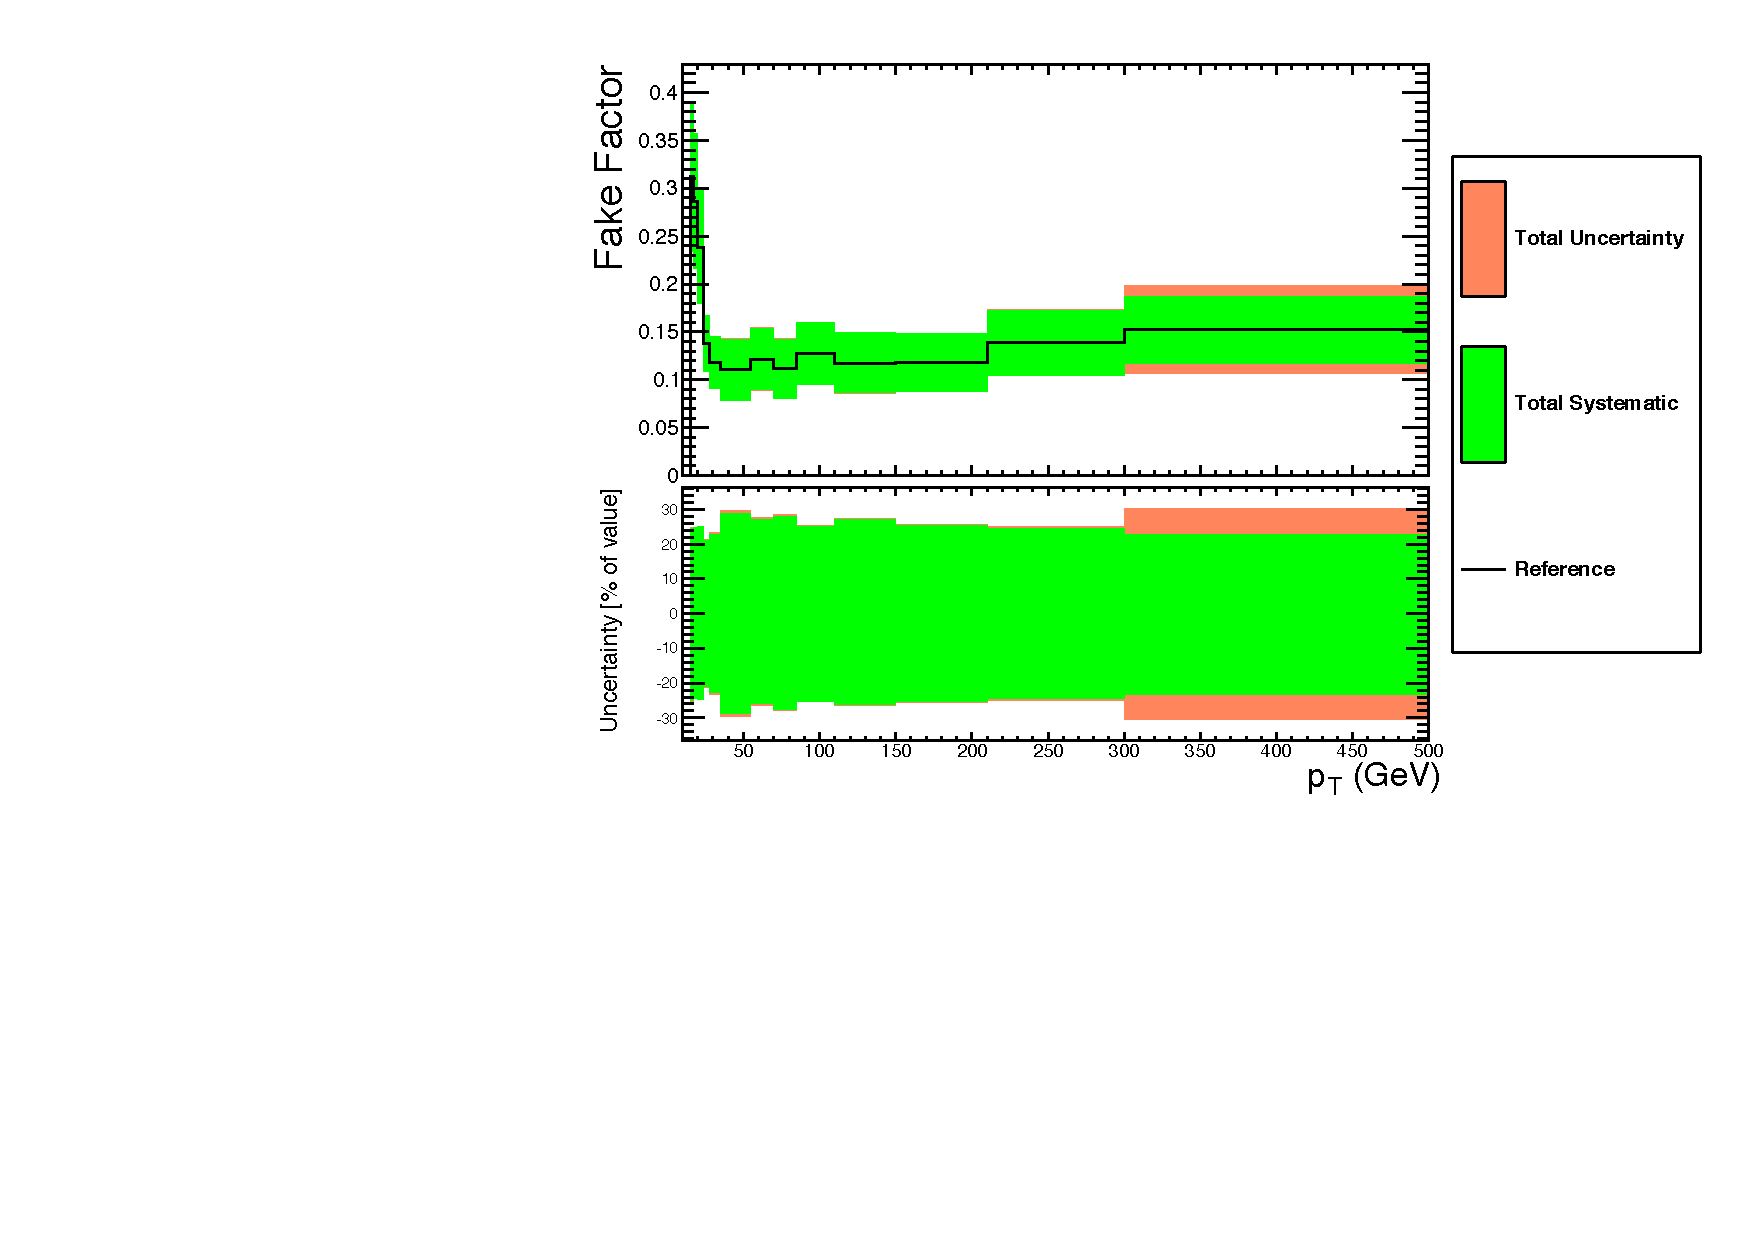
\includegraphics{figures/backgrounds/c_FinalFF_systematics_linearx_biggerlabels}}
  }
  \subfloat[Log scale] {
	\resizebox{3in}{!}{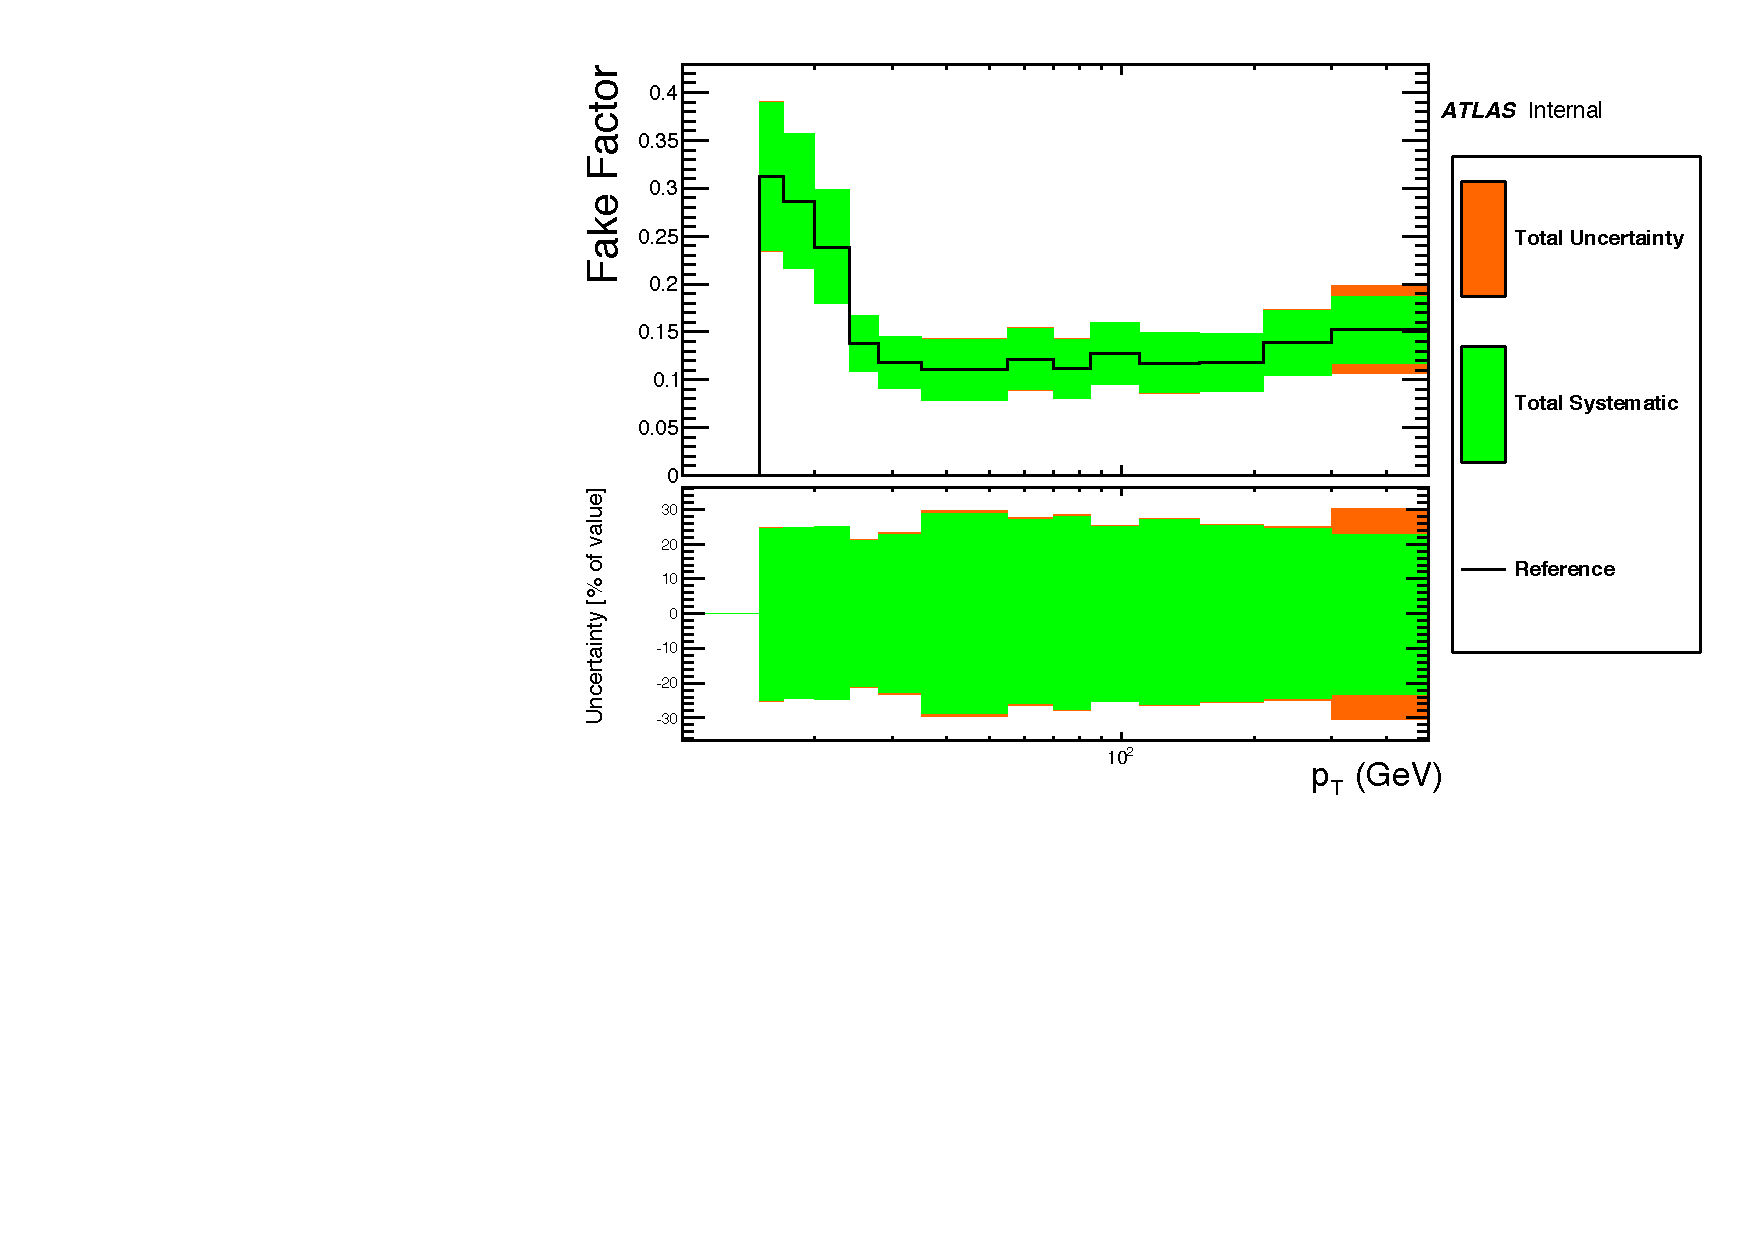
\includegraphics{figures/backgrounds/c_FinalFF_systematics_logx_biggerlabels}}
  }
  \caption{Electron fake factors vs. $\pt$ with systematic and total uncertainties. The statistical uncertainty includes both the data and prompt subtraction Monte Carlo statistics.}
  \label{fig:electron-fake-factor-uncertainties}
\end{figure}

\clearpage

\subsection{Muon Fake Factors}\label{sec:muon-fake-factors}
The muon fake factor method follows that used in the 2011 ATLAS same-sign dilepton search~\cite{TheATLASCollaboration:2012df}. The method targets non-prompt muons from semileptonic heavy flavor decays, punch-through, and decays-in-flight of long-lived mesons by inverting the isolation requirements. Specifically, the denominator muons are defined as follows:
\begin{itemize}
  \item Pass all numerator muon requirements in table~\ref{table:electron-muon-selections}, except the requirements on \verb.Etcone30., \verb.ptcone30., and $\frac{d_0}{\sigma_{d_0}}$. 
  \item Loosen impact parameter cut:
  \begin{equation}
	|\frac{d_0}{\sigma_{d_0}}|<10
  \end{equation}
  \item Invert isolation:
  \begin{align}
	\etcones{30},\ \ptcones{30} &> \left\{\begin{array}{ccc} 0.15 \pt & : & \pt<100~\mbox{GeV} \\ 15+0.01 \pt~\mbox{GeV} & : & \pt>100~\mbox{GeV} \end{array} \right. \\
	\etcone{30} &< 2.0 \\
	\ptcone{30} &< 2.0 \\
  \end{align}
  \item If $\pt<40~\mbox{GeV}$, apply the same overlap requirement as the signal regions, removing the muon if $\Delta R (\mu,\ \mbox{jet})<0.3$. This overlap requirement is not applied for muons with $\pt>40~\mbox{GeV}$, which increases the statistical precision at the expense of additional systematic uncertainty. This is denoted by ``dR'' or ``non-dR'' below, for example in figure~\ref{fig:MuFake_ff_1D}.
\end{itemize}

The muon fake factors are measured in a same-sign dimuon sample, triggered by the \verb.EF_2mu13. trigger. The use of same-sign muons suppresses the prompt contamination from $Z/\gamma^{*}$ events. The measurement uses only muons with large track impact parameter significance, $|\frac{d_0}{\sigma_{d_0}}|>3$, to obtain a sample enriched in non-prompt muons (if both muons satisfy this requirement, then both are counted in the measurement). An extrapolation factor is derived from Monte Carlo to account for the fact that the signal region requires $|\frac{d_0}{\sigma_{d_0}}|<3$, as detailed below.

Two sets of fake factors are measured, depending on the jet activity in the event. In the following, jets are required to have $\pt>30~\mbox{GeV}$, and be separated from muons with $\Delta R(\mu,\ \mbox{jet})>0.3$. 
\begin{itemize}
  \item \textbf{Inclusive}: Applied to events with zero jets. The measurement uses the entire same-sign dimuon sample.
  \item \textbf{Two-Jet}: Applied to events with one or more jet. The measurement uses same-sign dimuon events with at least two jets with $\pt>30~\mbox{GeV}$. 
\end{itemize}
Fake muons from the two-jet sample are expected to come primarily from $W+\mbox{jets}$ and $t\overline{t}$ processes, while the inclusive sample also includes contributions from $b\overline{b}$. Figure~\ref{fig:MuFake_stacks} shows the $\pt$ distributions of numerator and denominator muons in the measurement sample along with the expected prompt
contributions. 
\begin{figure}[h]
  \subfloat[Numerators, 0-jet]{
	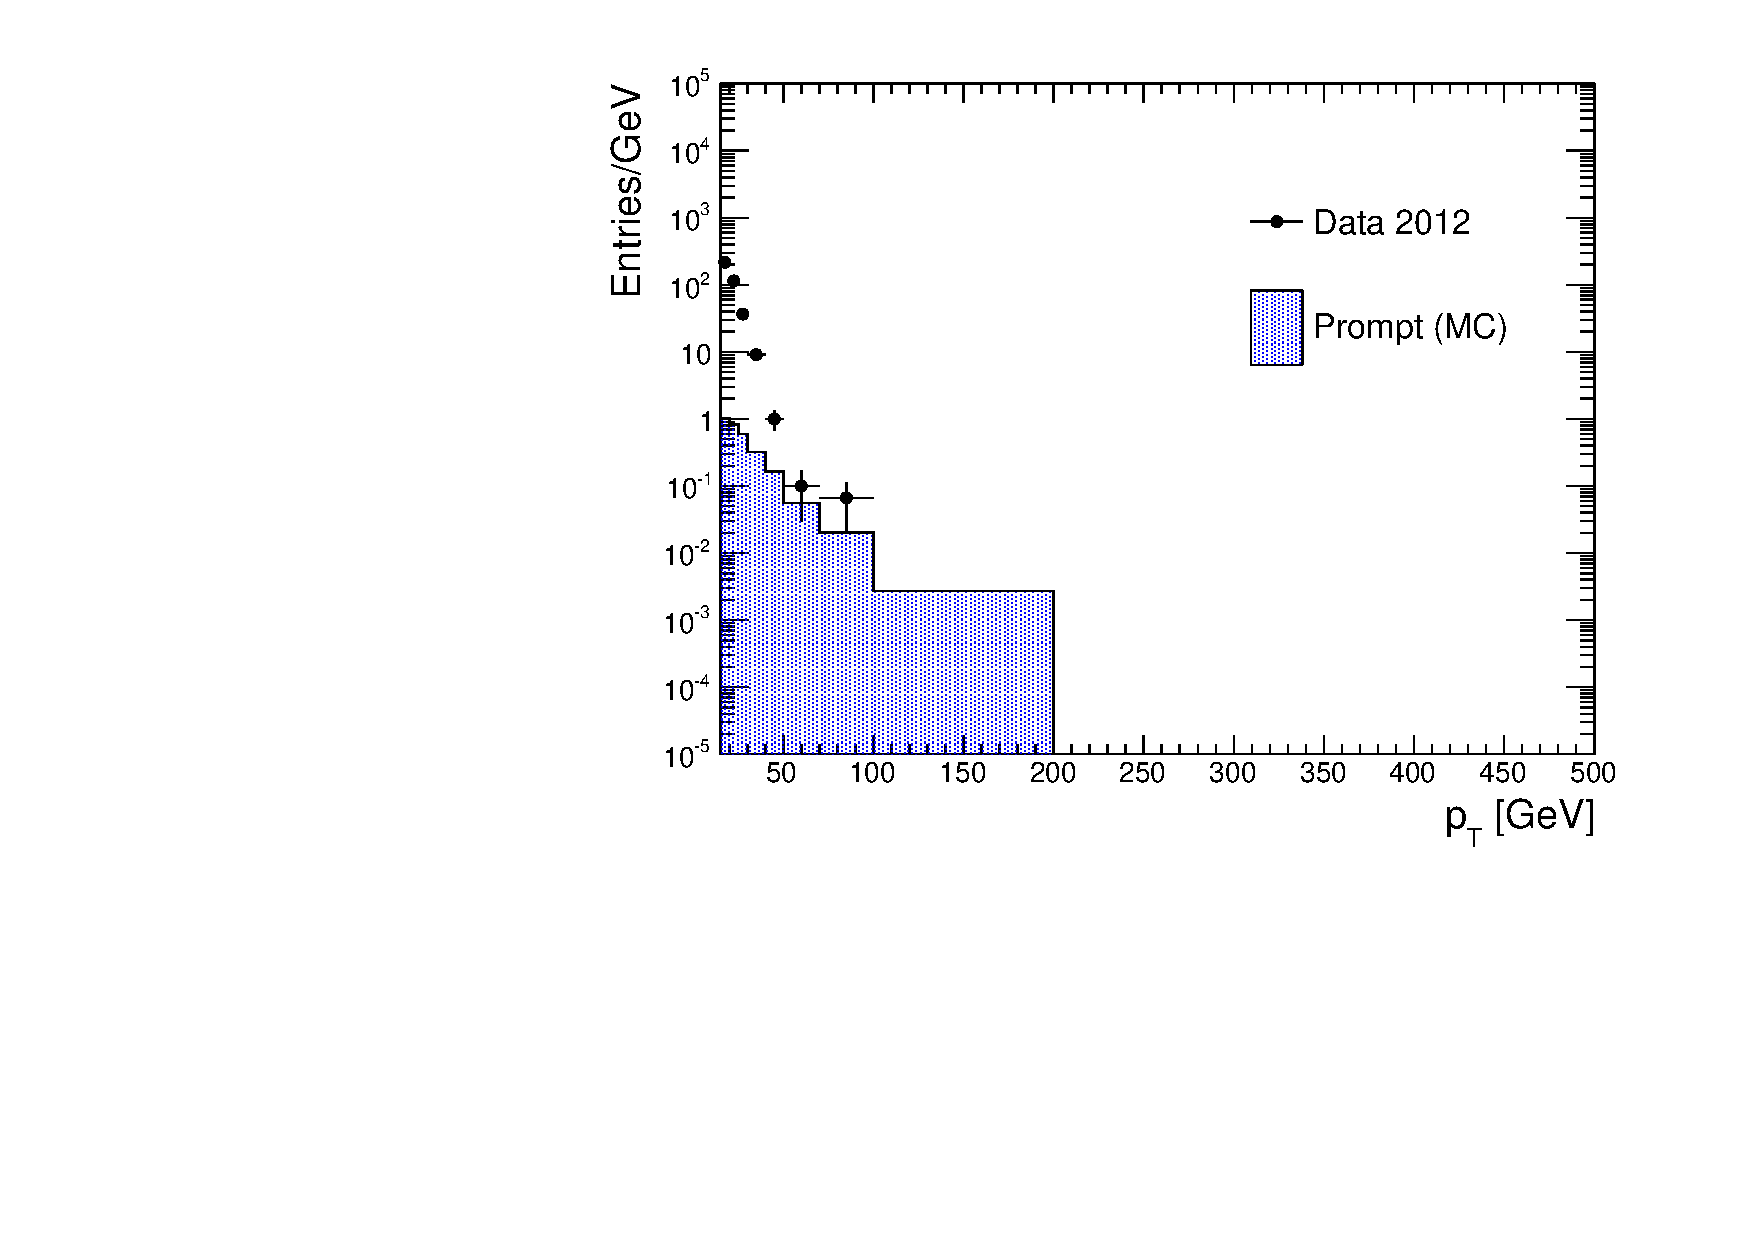
\includegraphics[width=0.3\columnwidth]{figures/backgrounds/num__0jet__nodr}
  }
  \subfloat[Numerators, 1-jet]{
	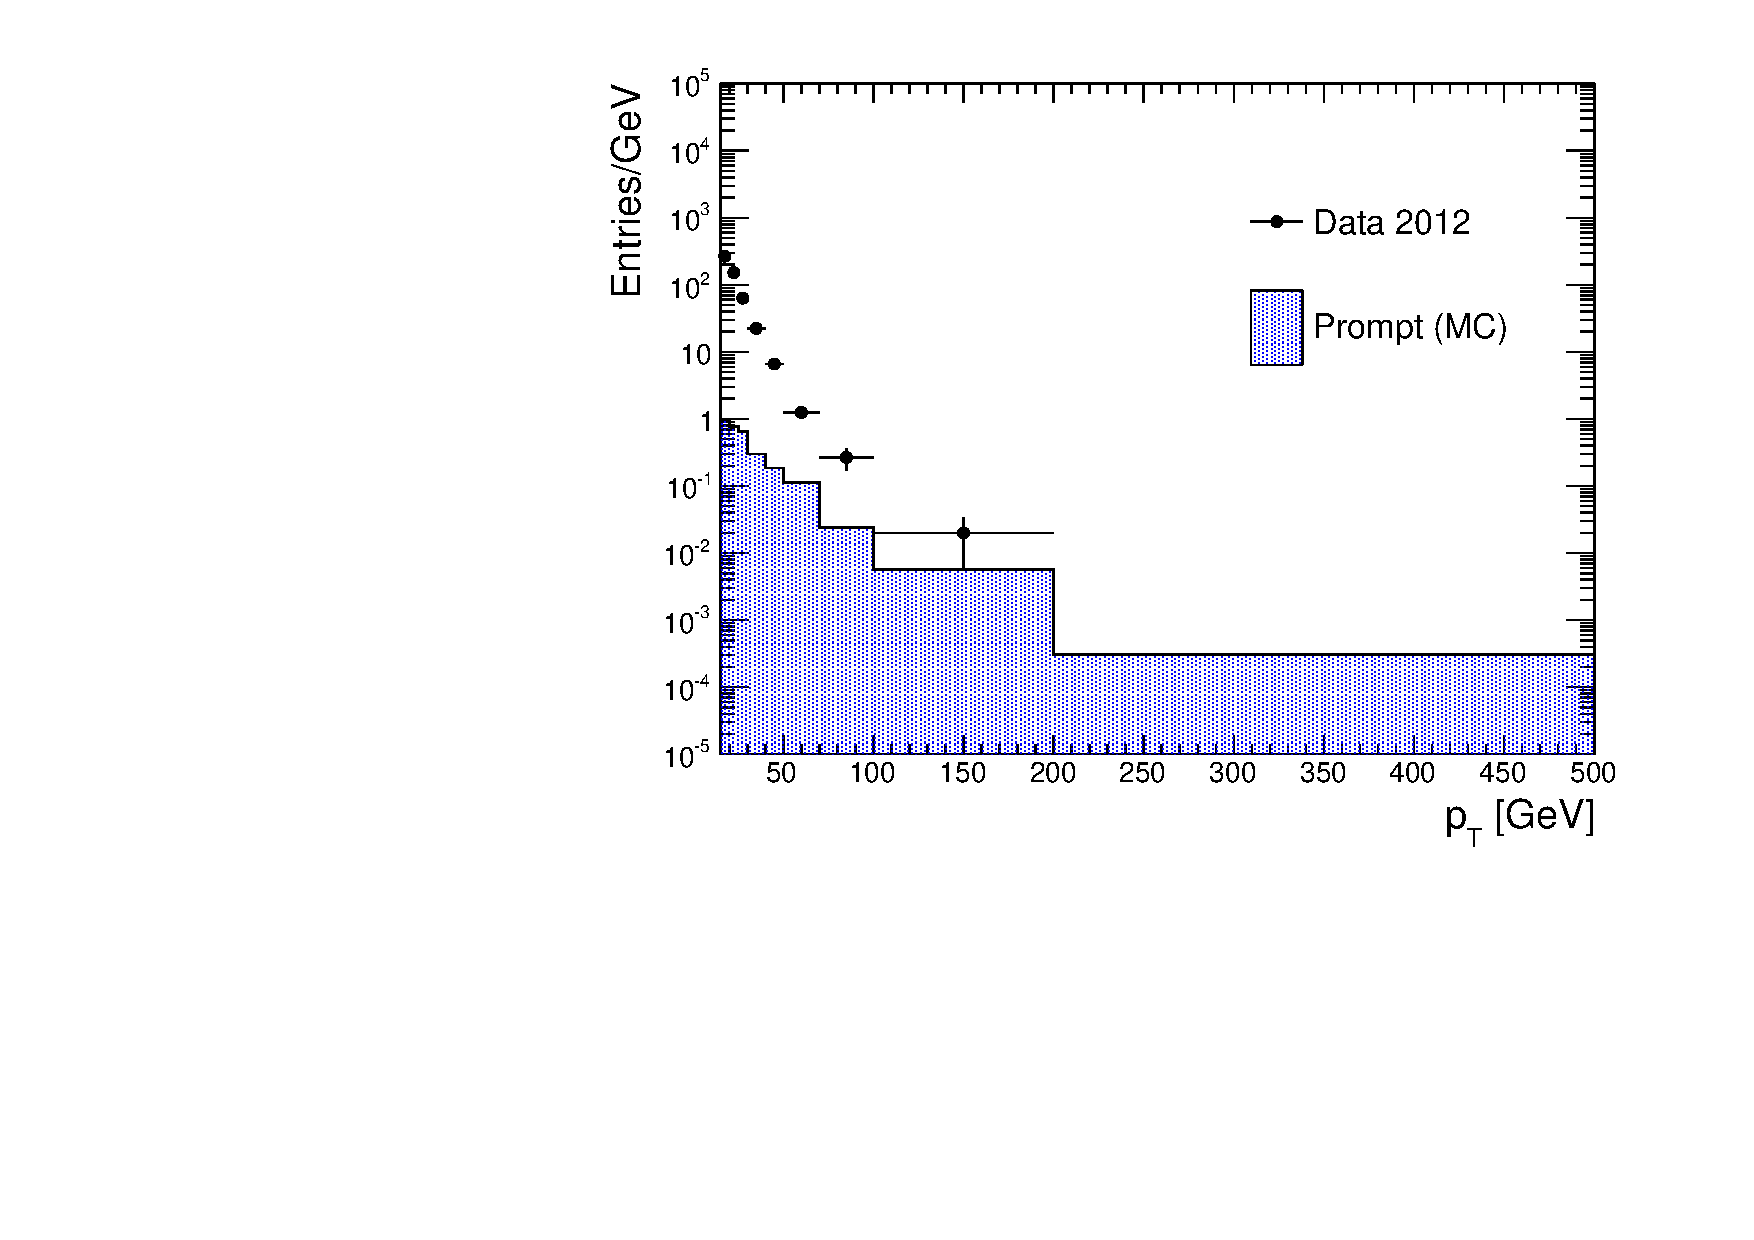
\includegraphics[width=0.3\columnwidth]{figures/backgrounds/num__1jet__sldr}
  }
  \subfloat[Numerators, 2-jet]{
	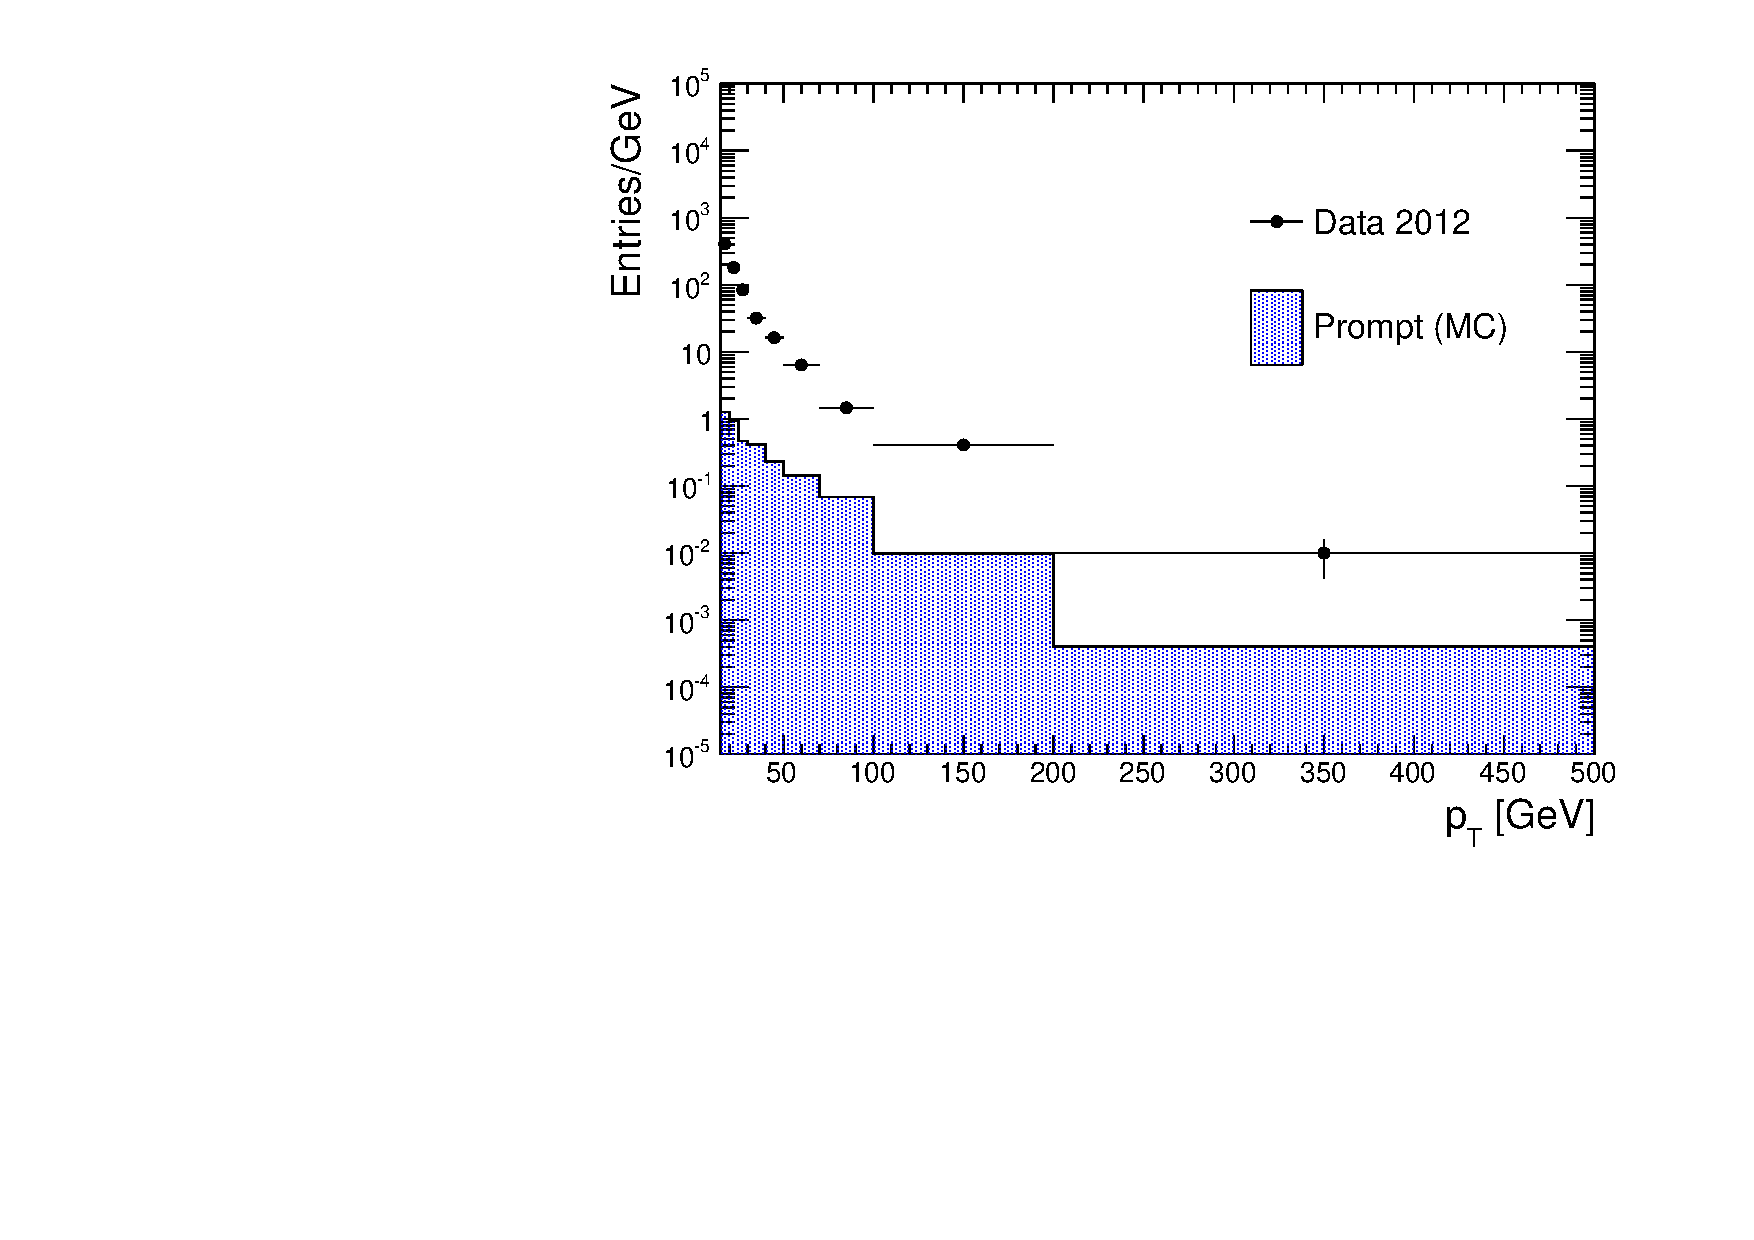
\includegraphics[width=0.3\columnwidth]{figures/backgrounds/num__2jet__sldr}
  }\\
  \subfloat[Denominators, 0-jet]{
	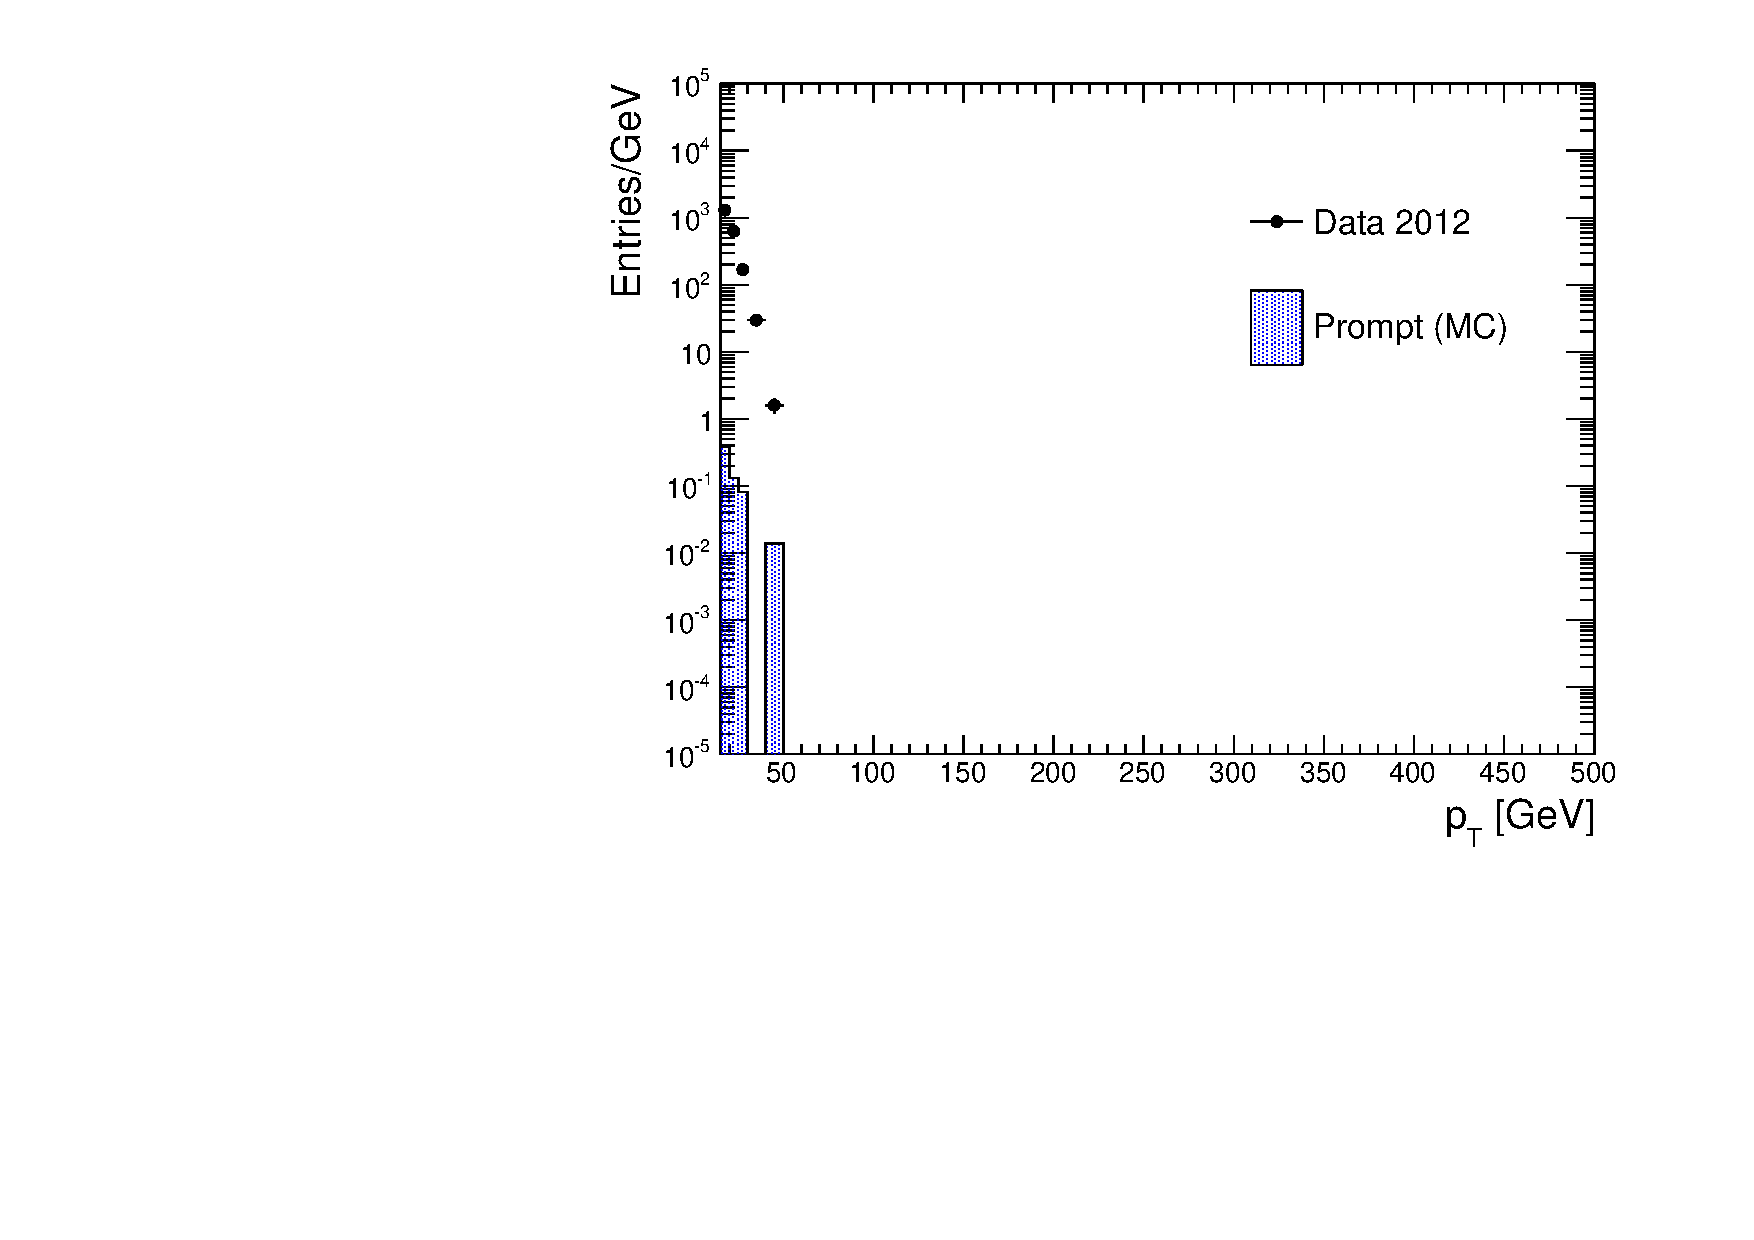
\includegraphics[width=0.3\columnwidth]{figures/backgrounds/den__0jet__nodr}
  }
  \subfloat[Denominators, 1-jet]{
	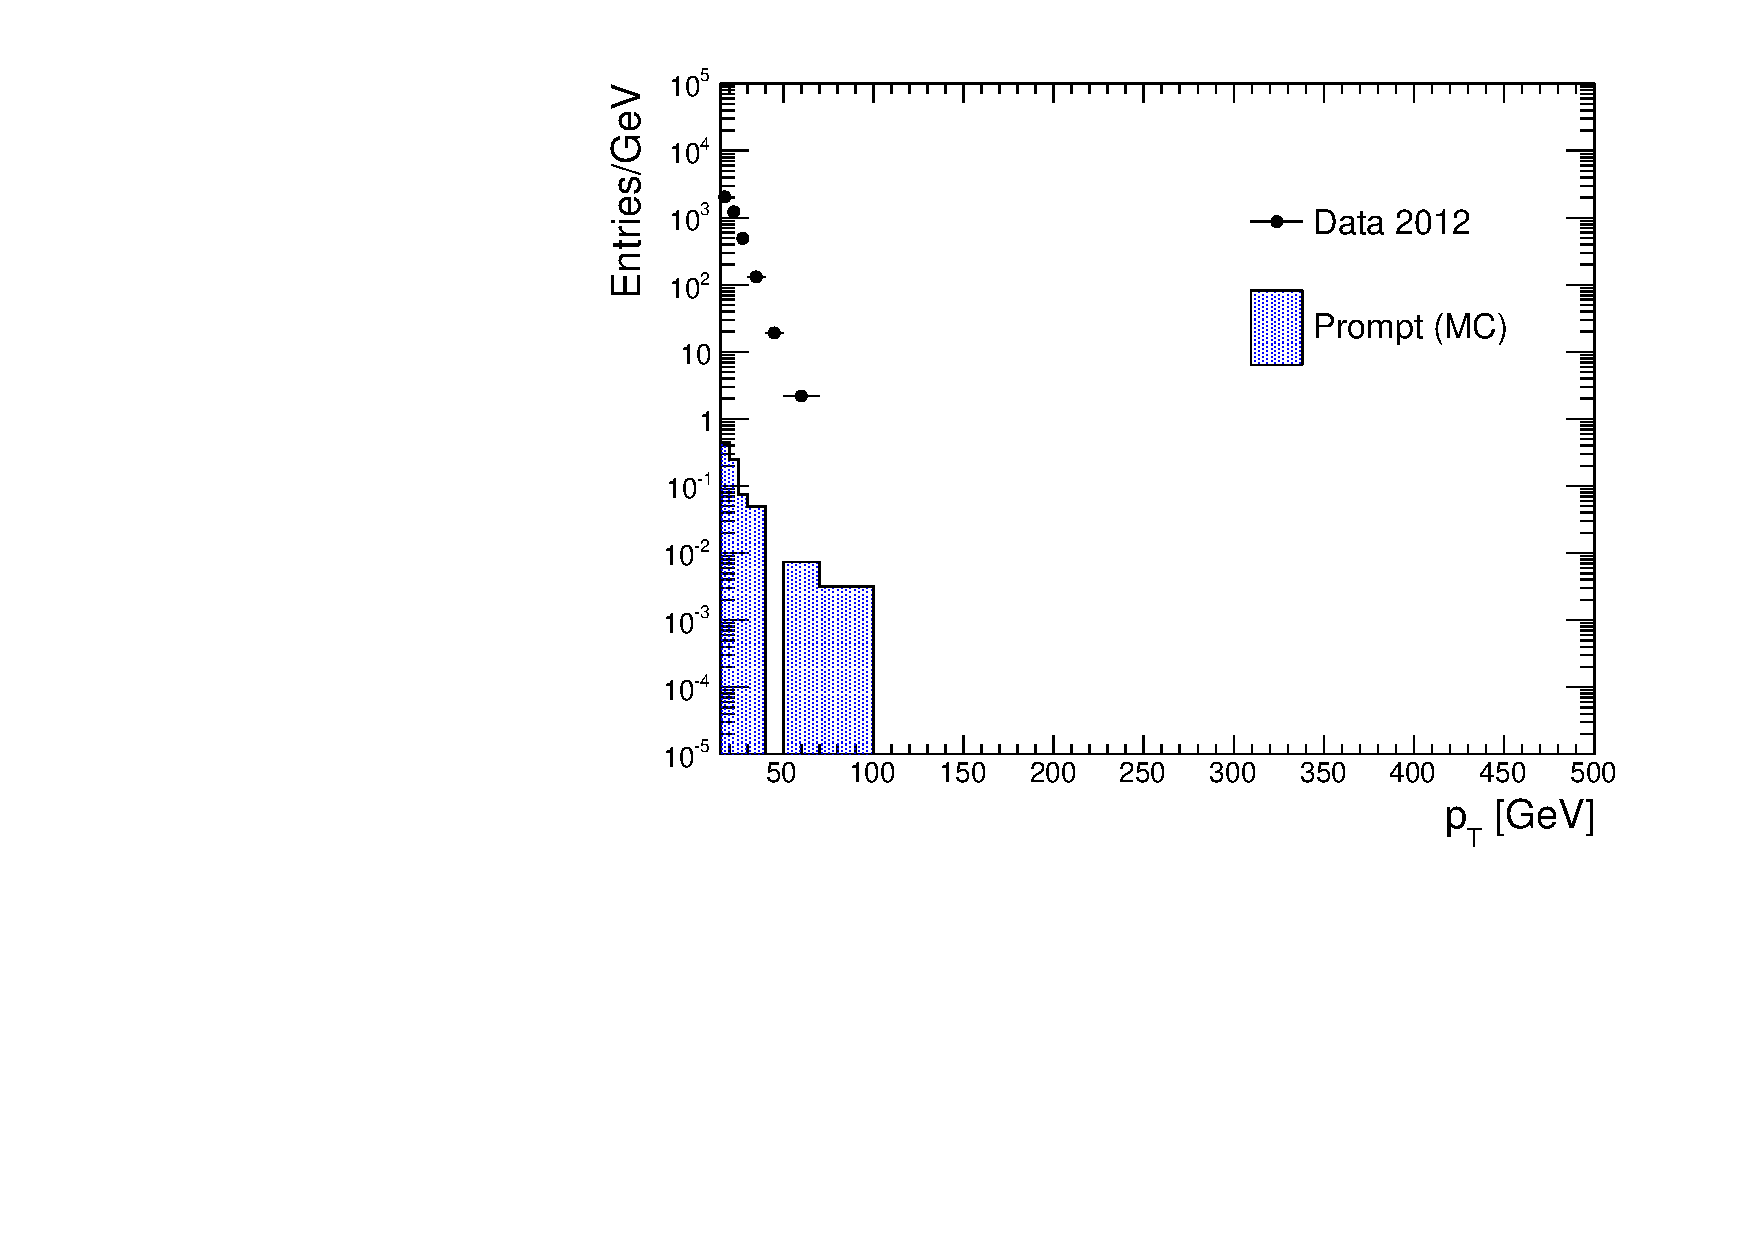
\includegraphics[width=0.3\columnwidth]{figures/backgrounds/den__1jet__sldr}
  }
  \subfloat[Denoninators, 2-jet]{
	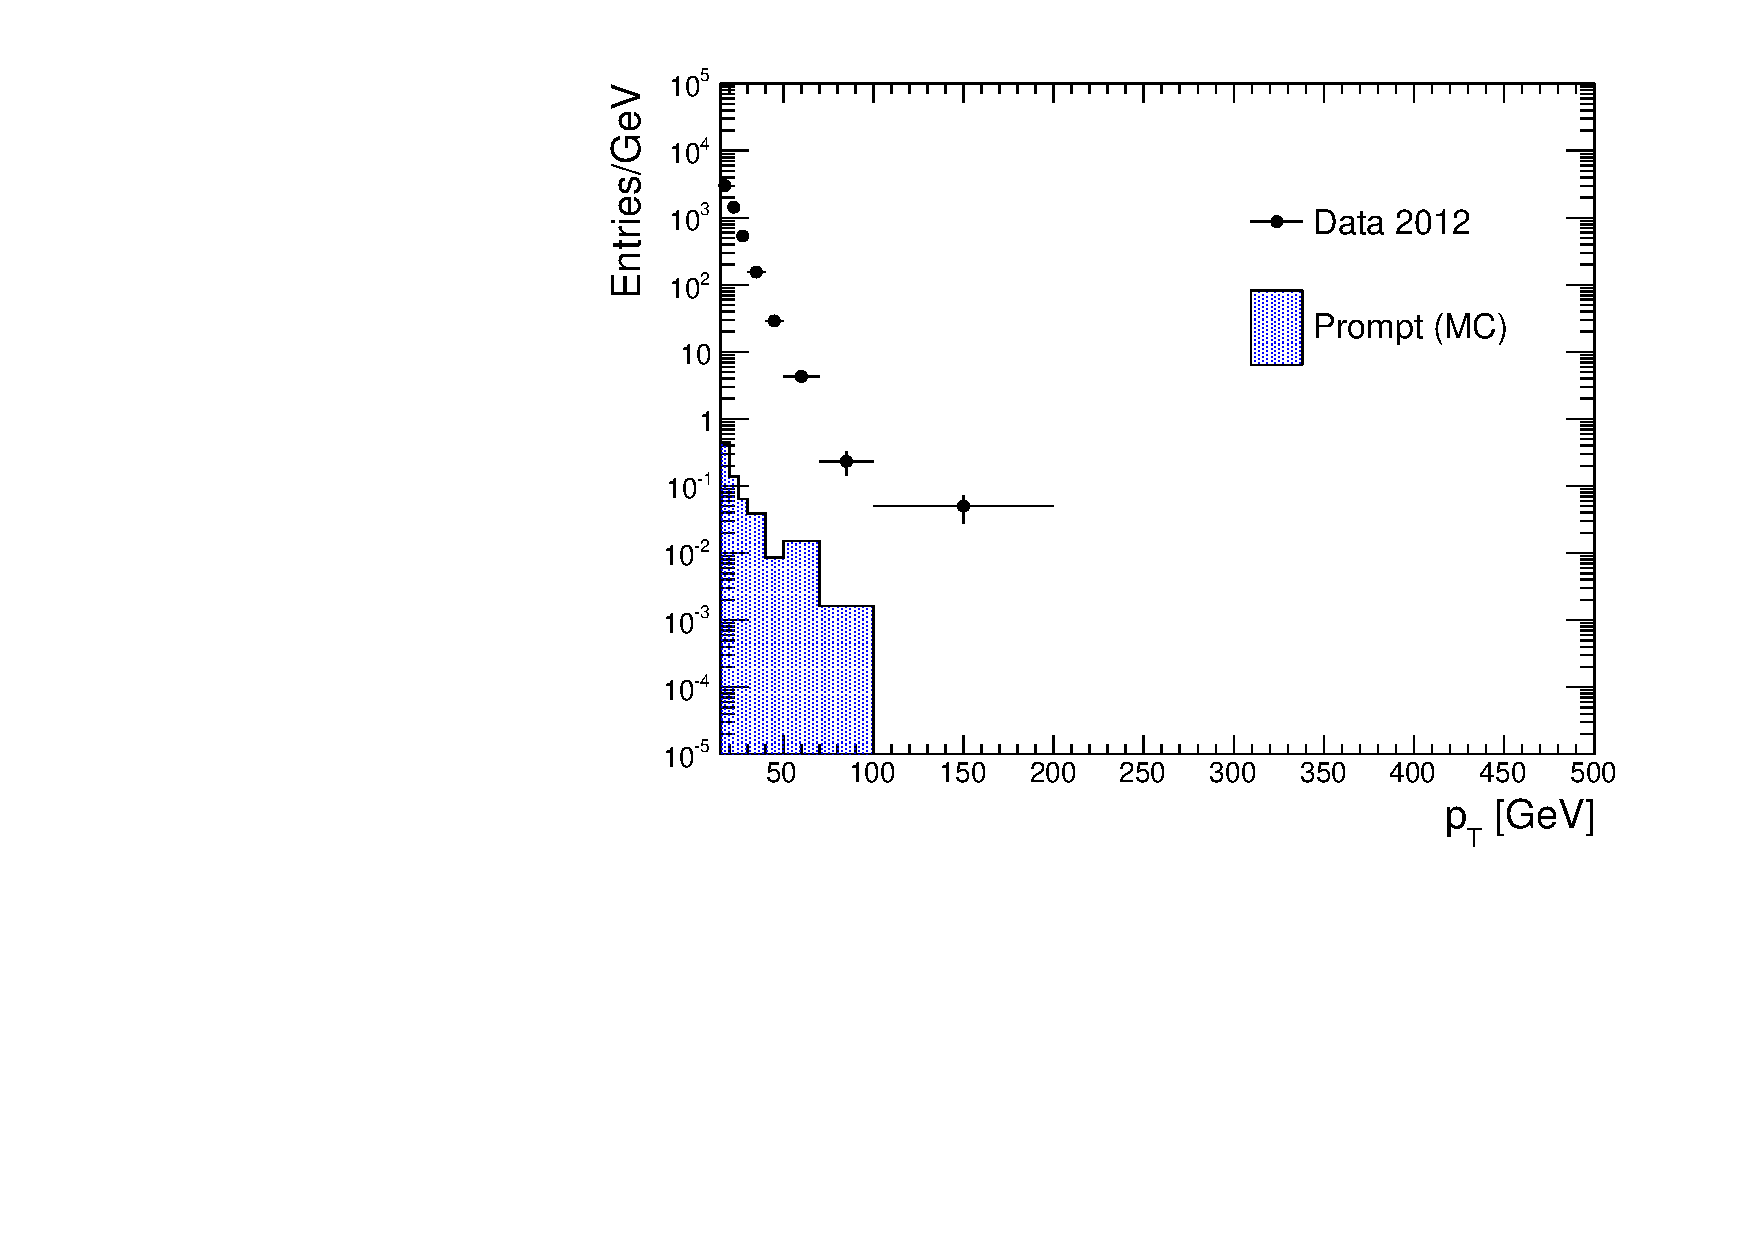
\includegraphics[width=0.3\columnwidth]{figures/backgrounds/den__2jet__sldr}
  }\\
  \subfloat[Denominators, 0-jet]{
	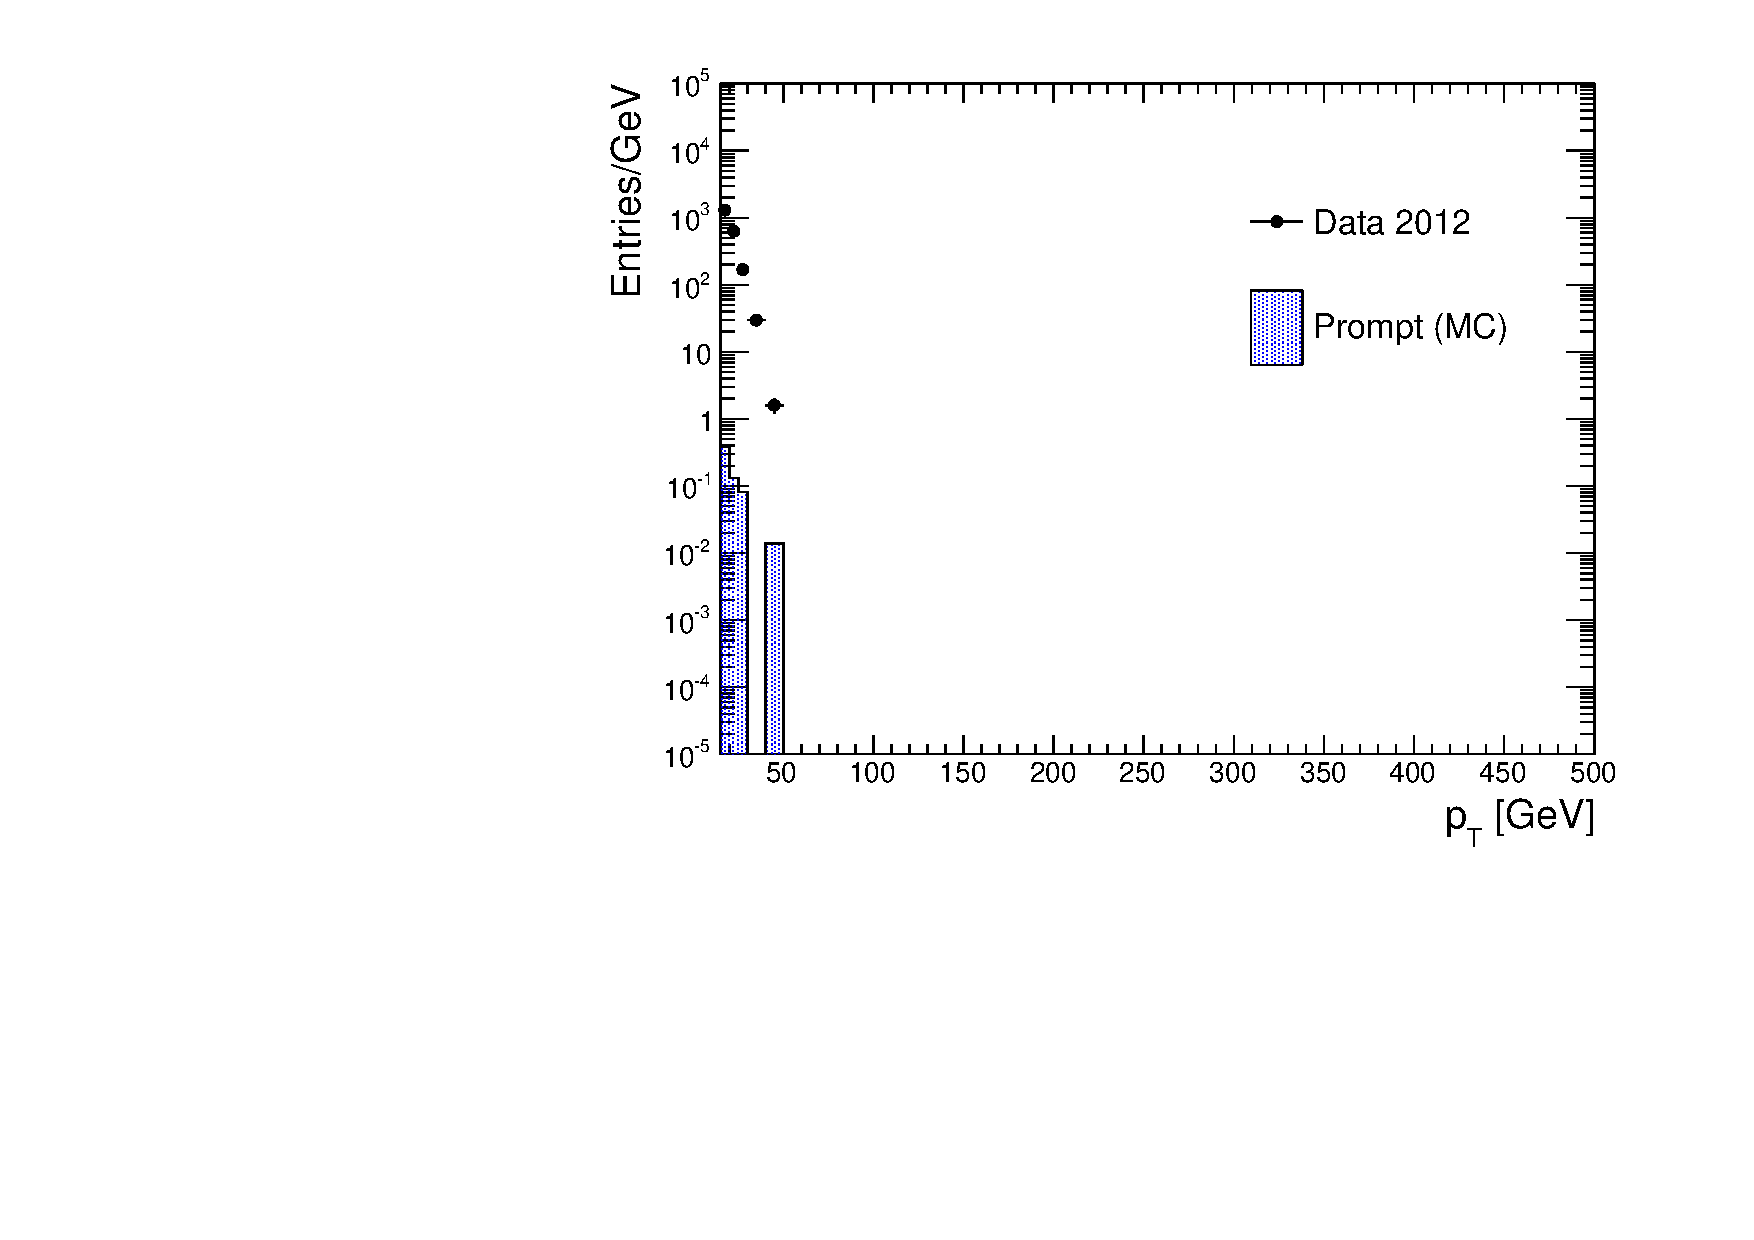
\includegraphics[width=0.3\columnwidth]{figures/backgrounds/den__0jet__nodr}
  }
  \subfloat[Denominators, 1-jet]{
	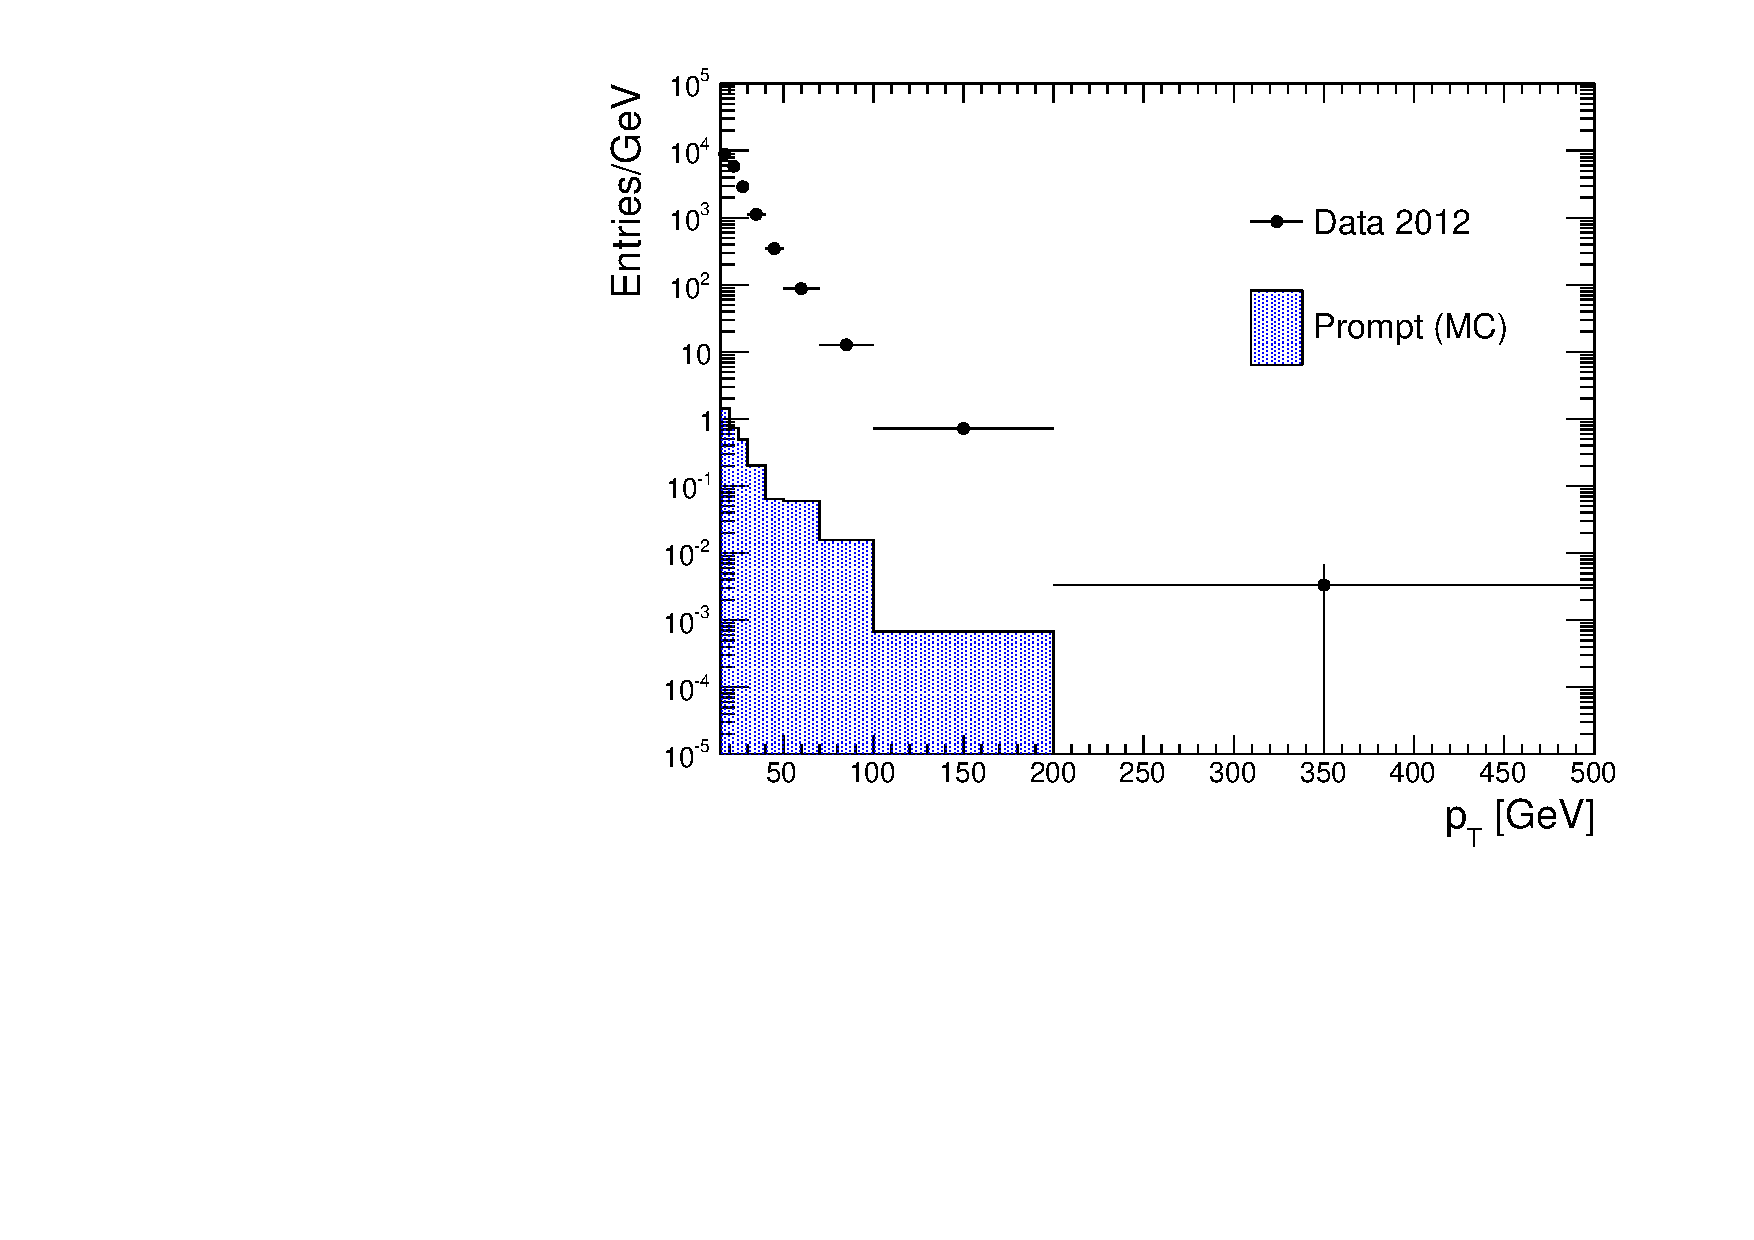
\includegraphics[width=0.3\columnwidth]{figures/backgrounds/den__1jet__nodr}
  }
  \subfloat[Denominators, 2-jet]{
	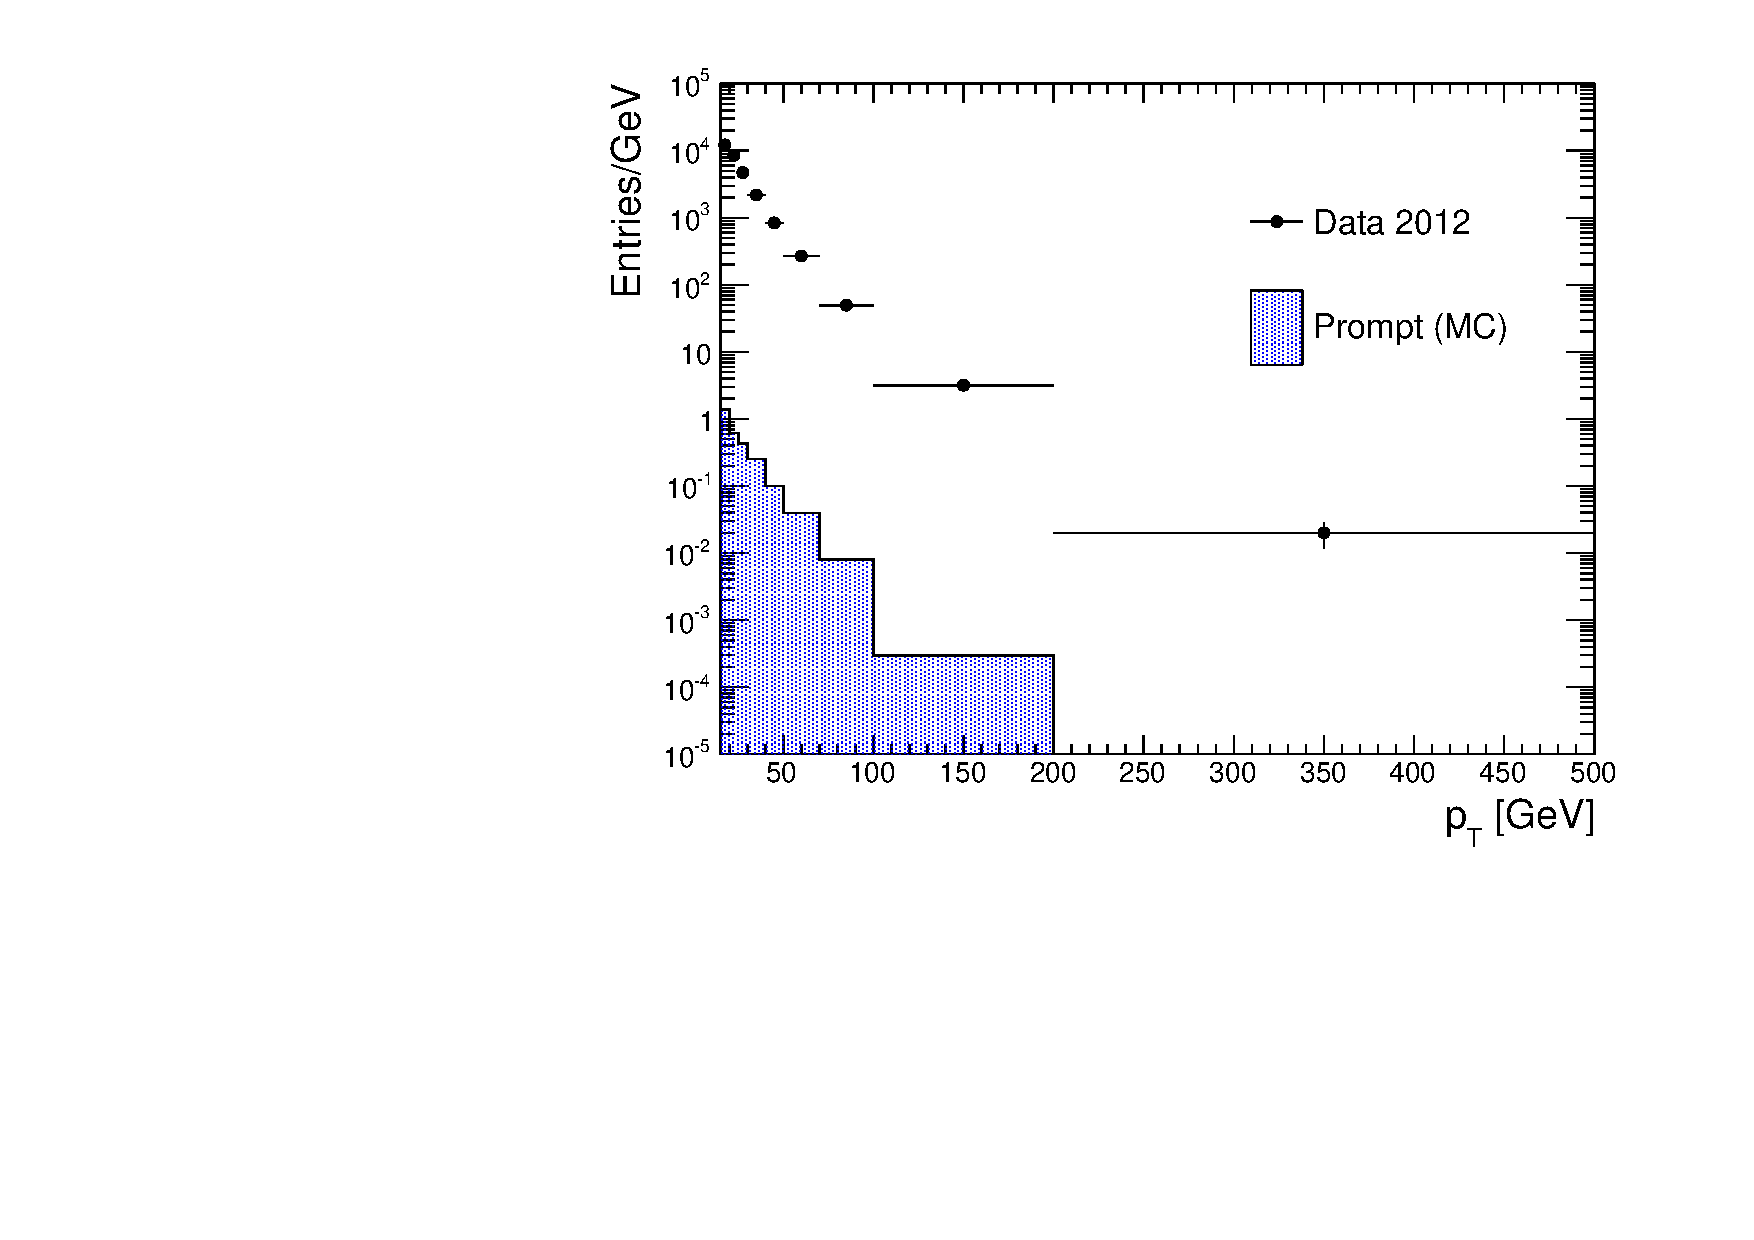
\includegraphics[width=0.3\columnwidth]{figures/backgrounds/den__2jet__nodr}
  }

  \caption{\label{fig:MuFake_stacks}$\pt$ spectrum of muons used in fake factor measurement.  The left plots show events with zero jets, the middle
	plots show events with one jet, and the right plots show events with two or more jets.  All numerator events require both numerator and denominator be separated from a jet by $\Delta R > 0.3$; the same requirement is applied to denominators in the second row of plots, while the third row shows 
denominators that are not required to be isolated from nearby jets.}
\end{figure}


The extrapolation factor from the measurement control region, with $|\frac{d_0}{\sigma_{d_0}}|>3$, to the signal region, with $|\frac{d_0}{\sigma_{d_0}}|<3$, is derived from various Monte Carlo samples. The extrapolation factor is simply the ratio of fake factors derived in Monte Carlo using the control region cut ($|\frac{d_0}{\sigma_{d_0}}|>3$) to those using the signal region cut ($|\frac{d_0}{\sigma_{d_0}}|<3$). The central value is taken from the \powheg\ $t\overline{t}$ sample, using all truth-level non-prompt muons, as shown in figure~\ref{fig:MuFake_extrap}. A systematic uncertainty is assigned by comparing with other samples (\mcatnlo\ $t\overline{t}$ and \pythiab\ $b\overline{b}$ and $c\overline{c}$), and using only same-sign dimuon events in these samples.  

\begin{figure}[h]
\centering 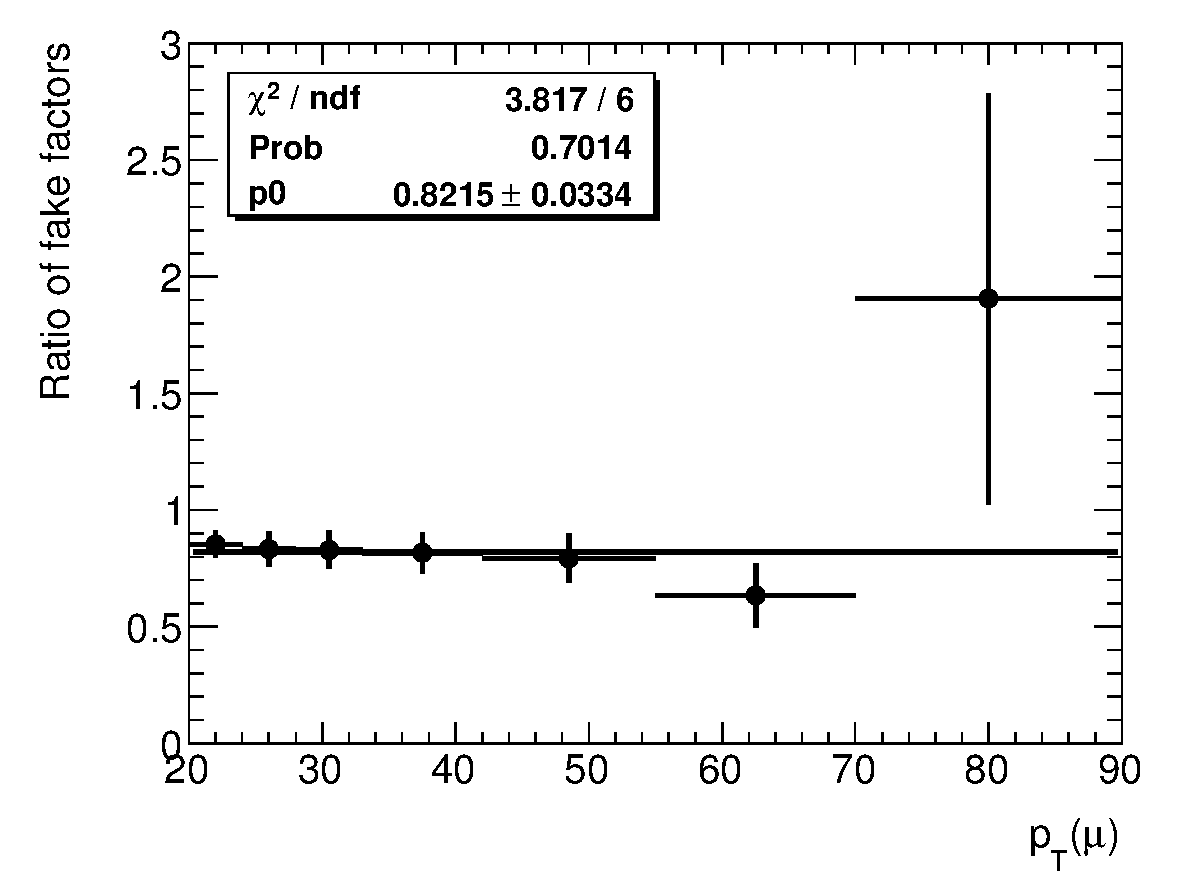
\includegraphics[width=0.48\textwidth]{figures/backgrounds/MuFake_extrap_ratio}
\caption{\label{fig:MuFake_extrap}Ratio between the fake factors for muons with $|d_0|/\sigma(d_0)>3$ compared to fake factor with nominal numerator and denominator definitions.  These fake factors are derived from a \powheg\ $t\bar{t}$ sample.}
\end{figure}

The fake factors are parametrized one-dimensionally in $\pt$ and $\eta$, as there are insufficient statistics to do a full two-dimensional parametrization. The fake factor is computed as:
\begin{equation}
f(\pt,\ \eta) = \frac{f(\pt)\times f(\eta)}{\langle f \rangle}
\end{equation}
where $\langle f \rangle$ is the total average fake factor. The measured fake factors are shown in figures~\ref{fig:MuFake_ff_1D} and \ref{fig:MuFake_ff}. 

\begin{figure}
\centering 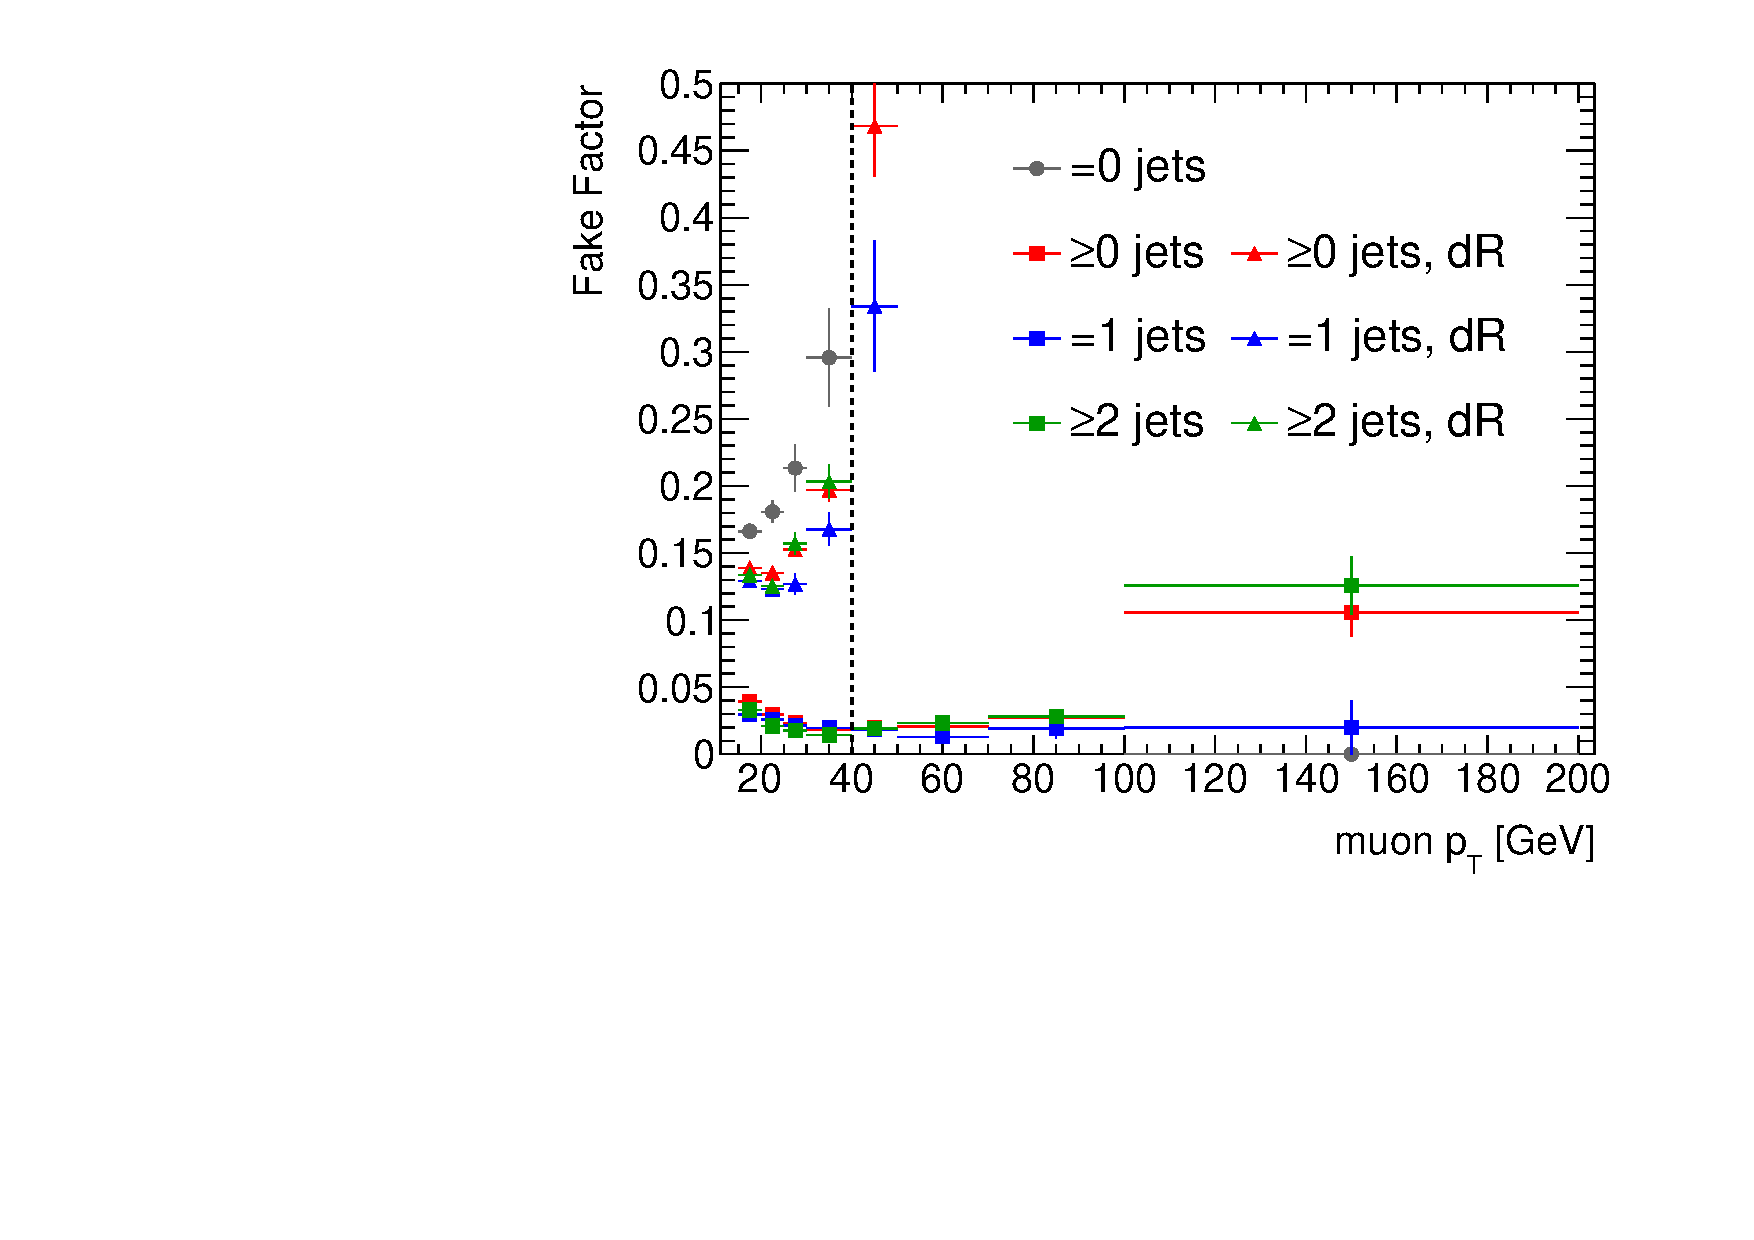
\includegraphics[width=0.48\textwidth]{figures/backgrounds/all_1D_pt}
%\centering \includegraphics[width=0.48\textwidth]{figures/backgrounds/MuFake_ff_vseta}
\caption{\label{fig:MuFake_ff_1D}Muon fake factors as a function of $\pt$. Two sets of fake factors are plotted, with and without the ``dR'' requirement. The vertical dashed line at 40 GeV indicates the point at which the fake factors switch from the ``dR'' points, where the denominators are required to be separated from nearby jets, to the lower, non-''dR'' points where the jet-isolation requirement is dropped to improve the statistics.}
\end{figure}

\begin{figure}
  \subfloat[Inclusive FF] {
	\resizebox{0.48\textwidth}{!}{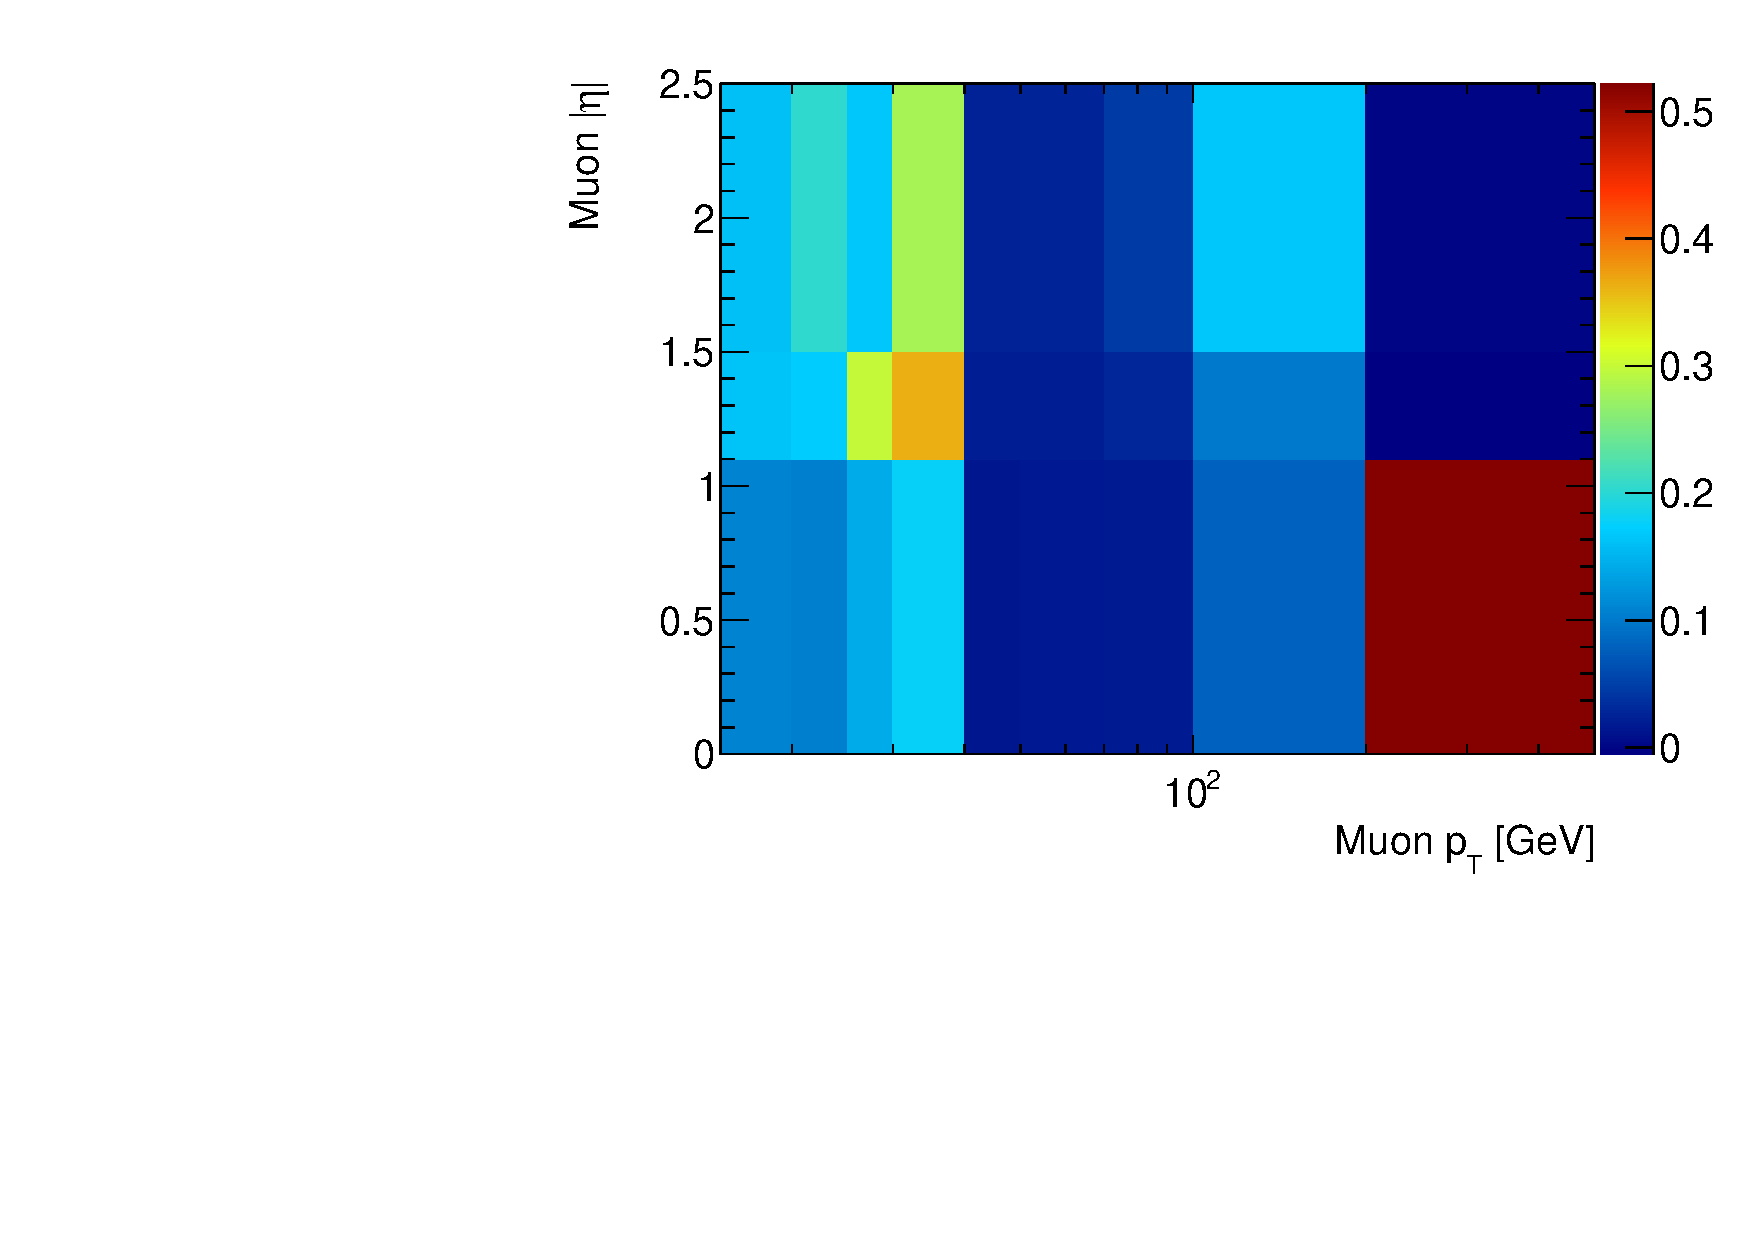
\includegraphics{figures/backgrounds/ff_0jet_final}}
  }
  \subfloat[Two-jet FF] {
	\resizebox{0.48\textwidth}{!}{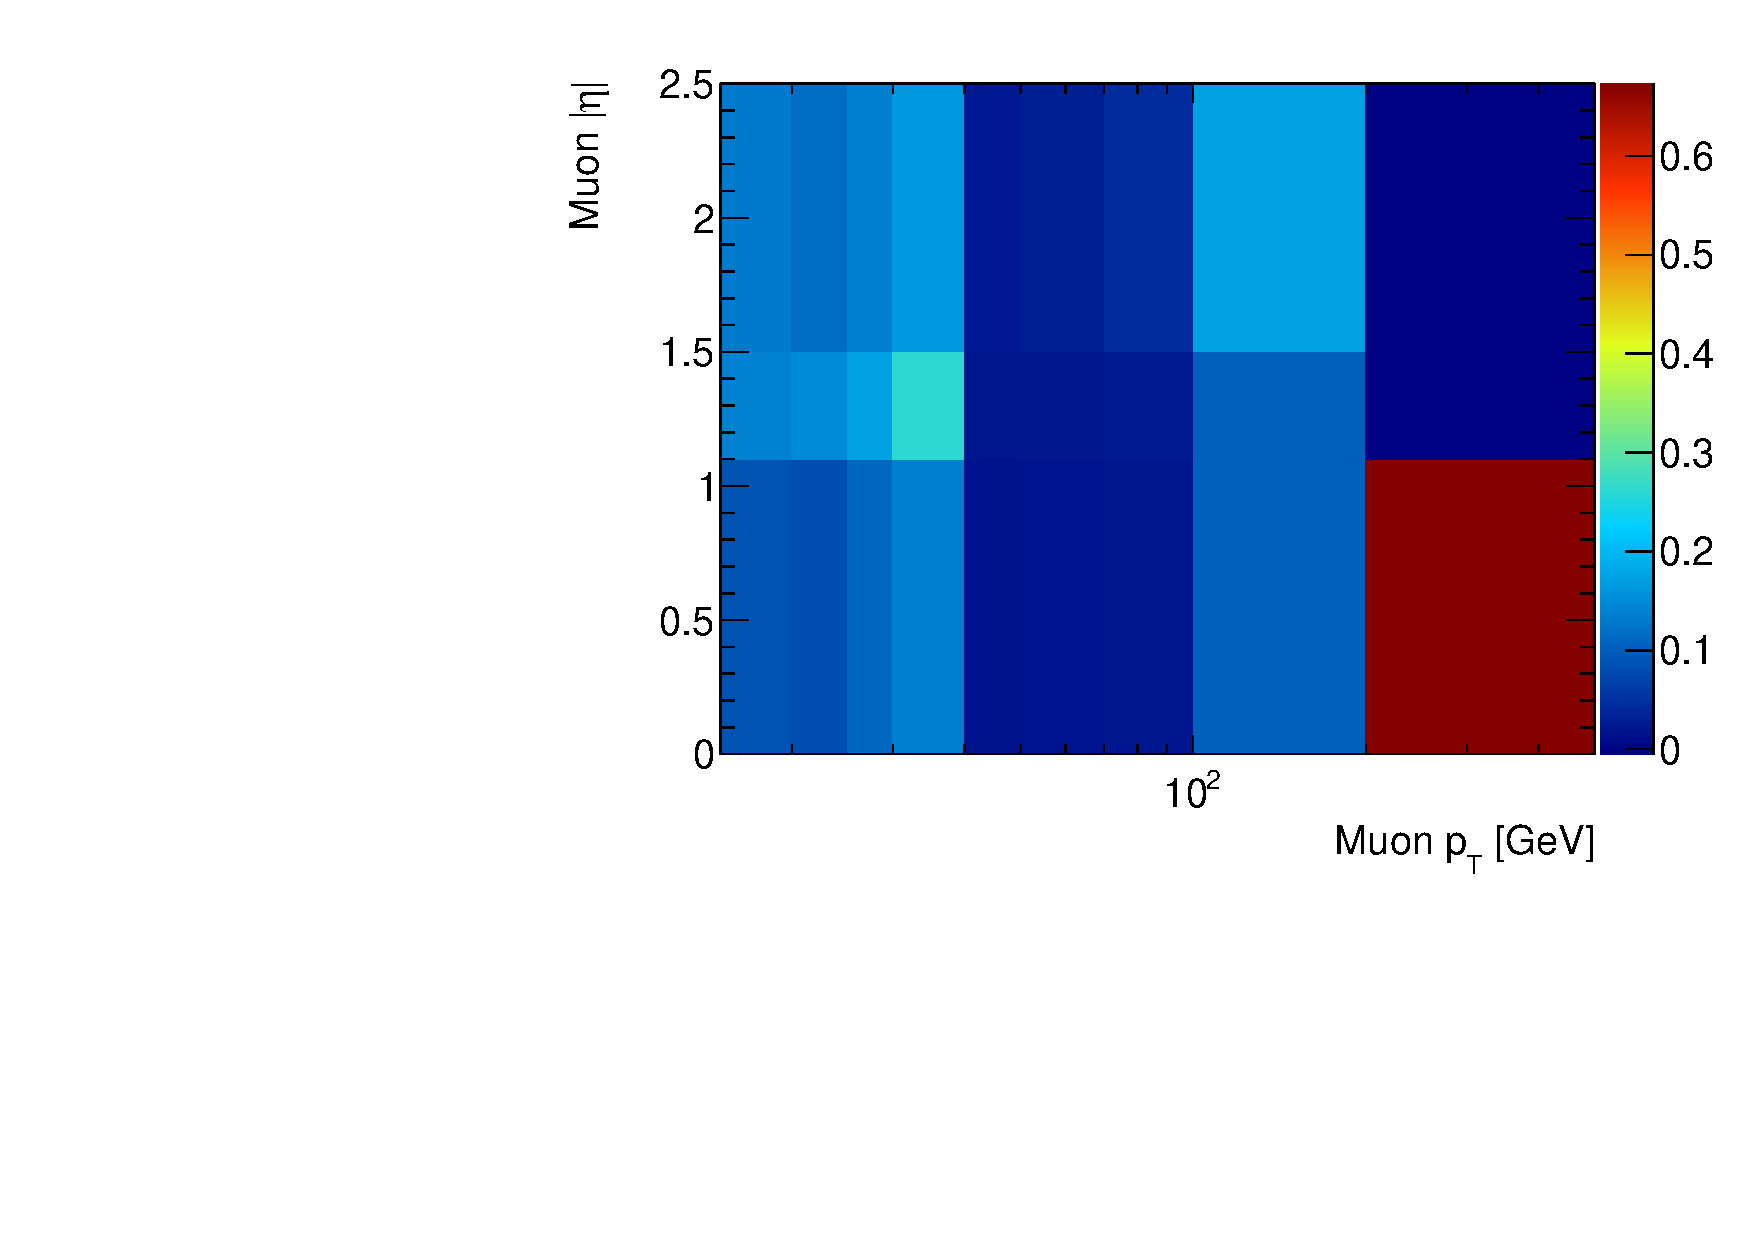
\includegraphics{figures/backgrounds/ff_2jet_final}}
  }
  \caption{Muon fake factors as functions of $\pt$ and $|\eta|$.  The left plot shows fake factors measured in the inclusive control sample and applied to events with zero jets. The right plot shows fake factors measured in events with two jets, and applied to events with at least one jet.}
  \label{fig:MuFake_ff}
\end{figure}


The sources of systematic uncertainty considered are listed below, and the fractional systematic uncertainty is shown in figure~\ref{fig:MuFake_syst}.

\begin{itemize}
  \item \textbf{Prompt subtraction}: The normalization of the simulated prompt subtraction samples is varied by $\pm10\%$, leading to a systematic uncertainty of $1$-$6\%$.
  \item \textbf{Topological dependence}: The difference between the inclusive and two-jet fake factors is taken as a systematic uncertainty. The uncertainty is symmetrized, using the full difference as both upward and downward uncertainty, and ranges from $3\%$ to $36\%$. 
  \item \textbf{Dependence on $d_0$ significance}: As mentioned previously, the extrapolation factor is derived in a number of different Monte Carlo samples. The largest deviation of $24\%$ is taken as a systematic uncertainty.
  \item \textbf{Light flavor fraction}: As with the electron fake factors, the fake factor values are quite different for muons originating from light flavor (LF) sources ($\pi/K$ decay or punch-through) versus heavy flavor (HF) decays. The systematic uncertainty is described in detail in \cite{DeViveiros:1670929}; in brief, it uses the difference in momenta measured by the inner detector and muon spectrometer as a discriminant between HF and LF fakes, estimates the difference in HF/LF fraction between the control and signal regions, and finally uses HF and LF fake factors measured in Monte Carlo to estimate the effect of the discrepancy in HF/LF fraction. A systematic uncertainty of $2\%$ to $21\%$ is assigned. 
\end{itemize}

\begin{figure}
  \centering
  \subfloat[ Inclusive FF] {
	\resizebox{0.48\textwidth}{!}{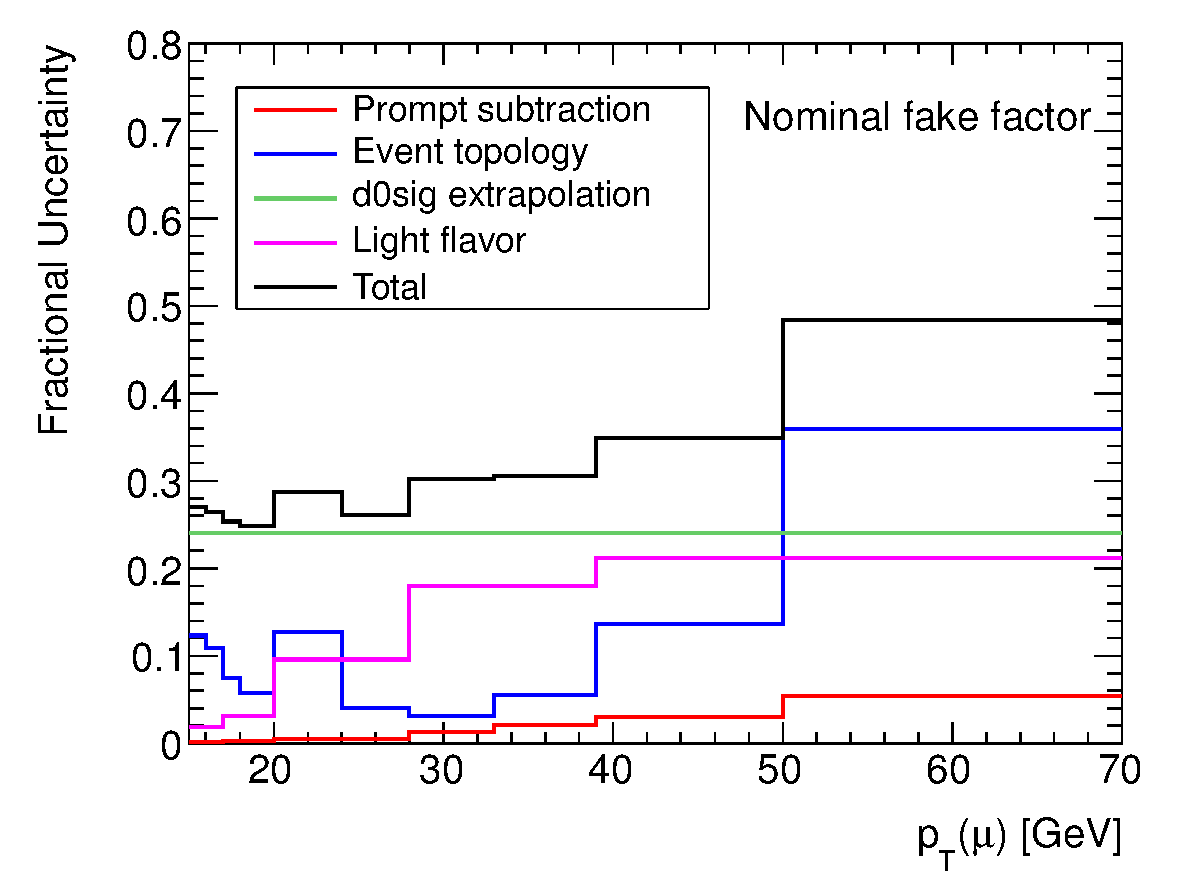
\includegraphics{figures/backgrounds/MuFake_syst_nom}}
  }
  \subfloat[ Two-jet FF] {
	\resizebox{0.48\textwidth}{!}{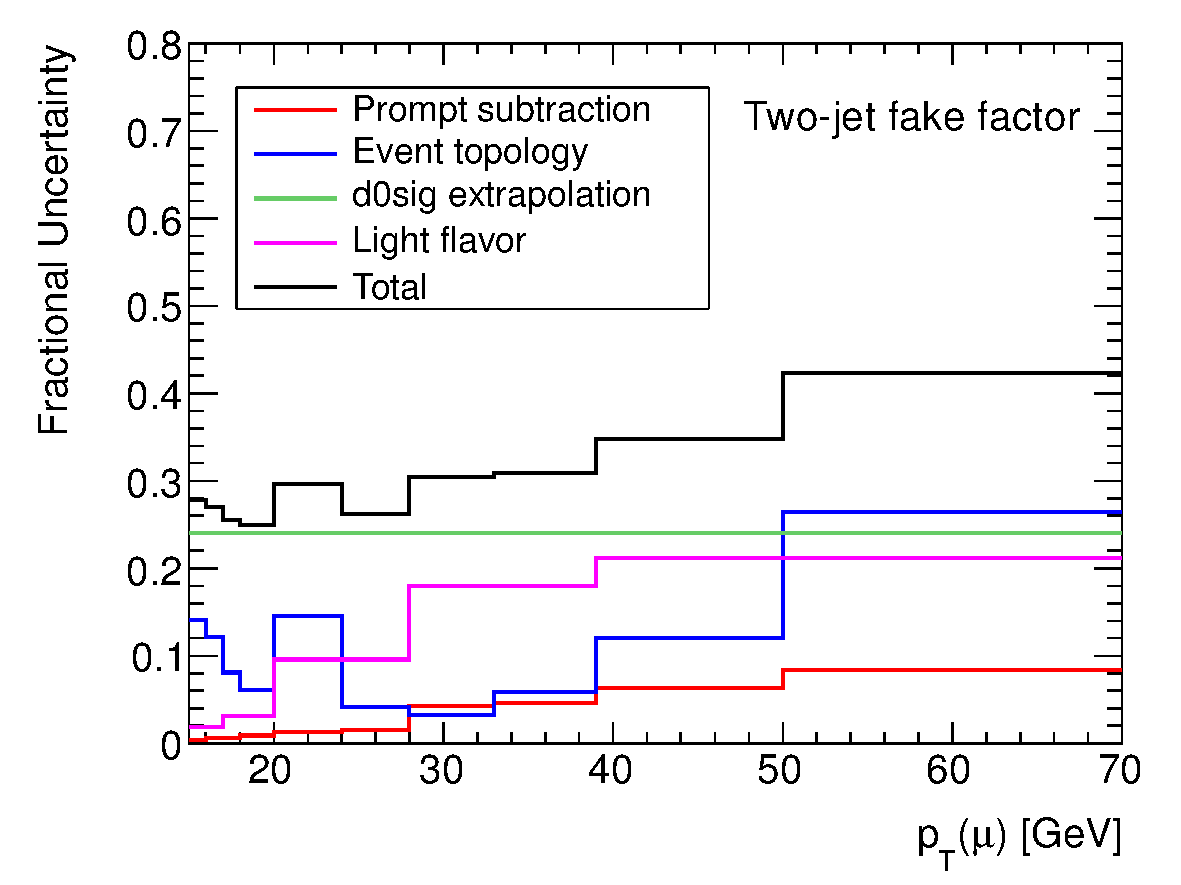
\includegraphics{figures/backgrounds/MuFake_syst_2jet}}
  }
  \caption{Systematic uncertainties on muon fake factor as a function of $p_{T}(\mu)$.  The left plot shows the uncertainties for the inclusive fake factor, while the right shows the uncertainty for the two-jet fake factor.}
  \label{fig:MuFake_syst}
\end{figure}



\subsection{Tau Lepton Fakes}\label{sec:ff-tau}
The detector signature of hadronically decaying tau leptons, consisting of a jet with one or more associated tracks, is not as distinctive as the signature of electrons and muons. Differentiating between jet, which are copiously produced in proton-proton collisions, and hadronically decaying tau leptons is difficult, and accordingly the reducible backgrounds in the 2L$+\tau_{\mathrm{had}}$ categories tend to be much larger than those in the 3L categories. 

\textcolor{red}{Lots of work to do here, to avoid copying and pasting PO's work!}

As taus can decay hadronically, their detector signature is not as distinctive as the one
associated with electrons and muons.  Therefore, jets, which are produced in abundance in
proton-proton collisions, are the main source of tau fakes, leading to large expected
fake-rates.  As the tau identification algorithms use multi-variate discriminants based on
calorimeter shower shapes and tracking information, the fake efficiency is strongly
dependent on the jet fragmentation. This in turn introduces a dependency of the fake-rates
on the parton initiating the jet (gluon, light-quark or heavy-quark).

Consequently, the fake-factors are less sensitive to the jet flavour if a tighter
efficiency working point is chosen for the denominator (as some shower shape requirements
are already applied).  However, it is important to still choose a working point that is
loose enough so that the denominator statistics are sufficiently large. A study of the
flavour-dependency of the fake-factors was performed in simulation samples.  For each jet
faking a $\tau$, the largest $p_{T}$ truth-particle present inside of the $\tau$
reconstruction cone was taken as an estimator of the parton initiating the jet.
Different denominator selections were chosen as a function of the existing loose
identification working point.  Denominators failing the \texttt{BDT-Medium} selection while
having a \texttt{BDTScore} larger than 0.7, 0.8, 0.9 or 1.0 $\times$ \texttt{BDTScore$_{Loose}$}
were all studied (where \texttt{BDTScore$_{Loose}$} is the $p_{T}$ dependent cut on the \texttt{  BDTScore} used by the $\tau$ identification algorithm).  Illustratively, each sequential
cut tightening denominator score reduces the statistics by a factor of roughly 2.  In the
end, the minimal threshold of 0.9 $\times$ \texttt{BDTScore$_{Loose}$} was chosen as it
offered a greatly reduced sensitivity to the flavour of the initiating parton in the jet,
while still offering large enough statistics for the sample. Further tightening of the cut
provided little improvement in flavour dependence. Using a $p_{T}$-dependent denominator
requirement ensures that the prompt efficiency is the same for all denominator taus, while
lowring the fake-factor dependent on $p_{T}$.

%A consequence of this choice of denominator is that the \met\ is incorrectly
%calibrated in events with denominator taus.  This is corrected in the analysis by
%modifying the \verb.RefJet. and \verb.RefTau. terms of \verb.MET_RefFinal. to use the tau
%energy instead of the jet energy.

The fake-factors are nominally parameterized as a function of the $p_{T}$ and $|\eta|$ of the
tau candidate, binned in 2 dimensions to preserve correlations. An additional scaling
correction is applied as a function of the highest \texttt{MV1} $b$-tagging weight of any jet
in the event.  The former two target dependencies associated with the jet shower shapes as a
function of kinematics and detector homogeinity.  The latter is taken to account for the
heavy-flavour component.

\subsection{Fake Factor Measurement}\label{sec:ff-tau-measurement}

It is also important to measure the fake-factors in a sample which is expected to have a
similar flavour composition as the signal regions used (the majority of trilepton events
with a fake tau are expected to come from electroweak production with an associated jet
faking the tau, for example $Z$ + jets events).  This is particularly important as no
observable can be used to directly and accurately classify each fake taus as potentially
gluon- or quark-initiated.
 
While the tau fake-factors were measured in the past from a $\gamma + $ jets sample, the
approach chosen for this iteration of the analysis is different.  
%Due to the increased
%pile-up conditions of the 2012 run, the purity of the photon sample is greatly
%compromised, leading to a larger contribution from multijet events, which then introduces
%a larger contribution from gluon-initiated jets, biasing the fake-factors.  
%Furthermore,
The low $p_{T}$ photon triggers were heavily prescaled during the 2012 run, limiting the
statistics available to measure fake-factors at low $p_{T}$ values.  Instead, a $W$ + jets
sample is used due to its high statistics and similar final-state kinematics.  A leading
numerator muon is required to be reconstructed as a tag (along with the associated trigger
requirement), and the fake-factors are then measured from the probe tau candidates.  No
other requirements are made on the events.  Alternatively, selection requirements could be
made to reject the main source of $\tau_{\mathrm{had}}$ prompts ($Z\rightarrow
\tau_{\mu}\tau_{\mathrm{had}}$), but such requirements can potentially introduce a bias on
the fake-factors (for example, introducing a same-sign requirement is expected to
drastically reduce the quark-initiated jet contribution).  Instead, the contribution from
prompt $\tau_{\mathrm{had}}$ is subtracted directly from Monte Carlo simulations.  The two
non-negligible contributions come from $Z$ + jets and $t\bar{t}$ events.

\begin{figure}
\centering 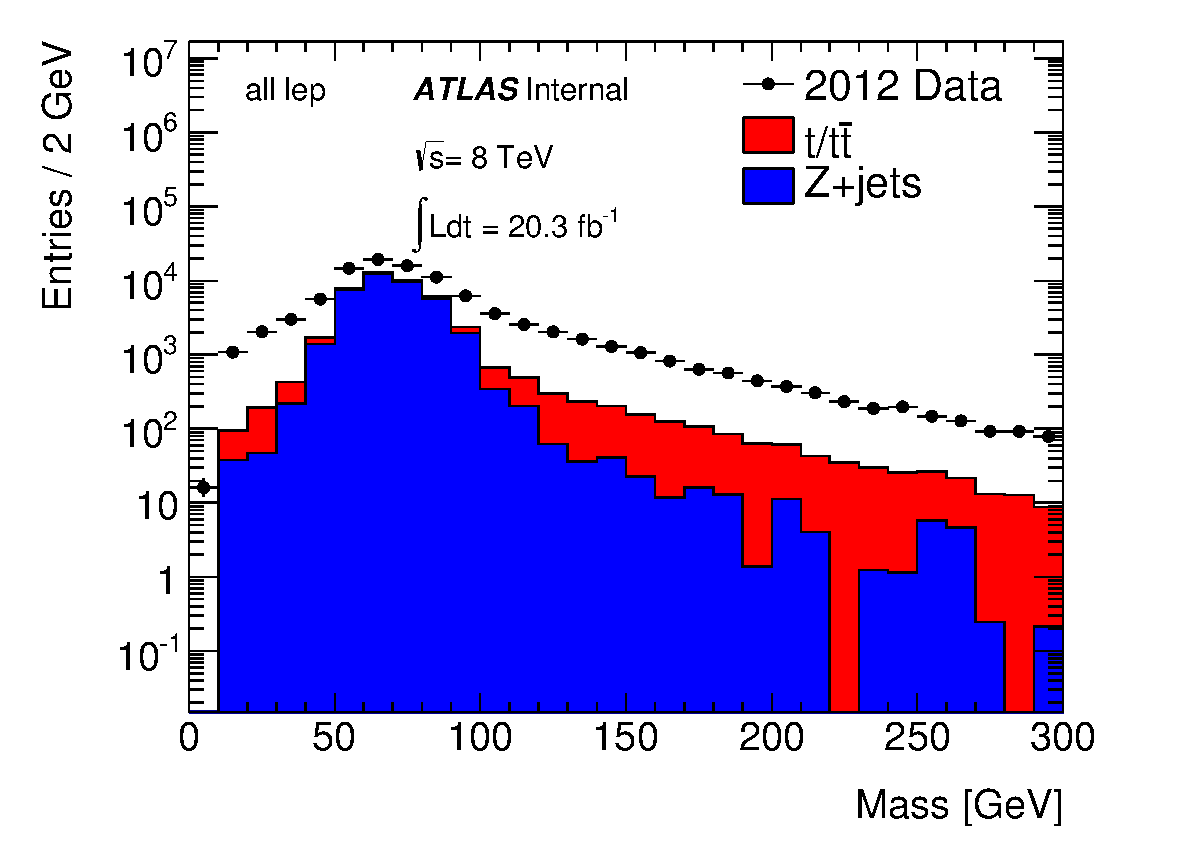
\includegraphics[width=0.48\textwidth]{figures/backgrounds/TauFakes_NumM}
\centering 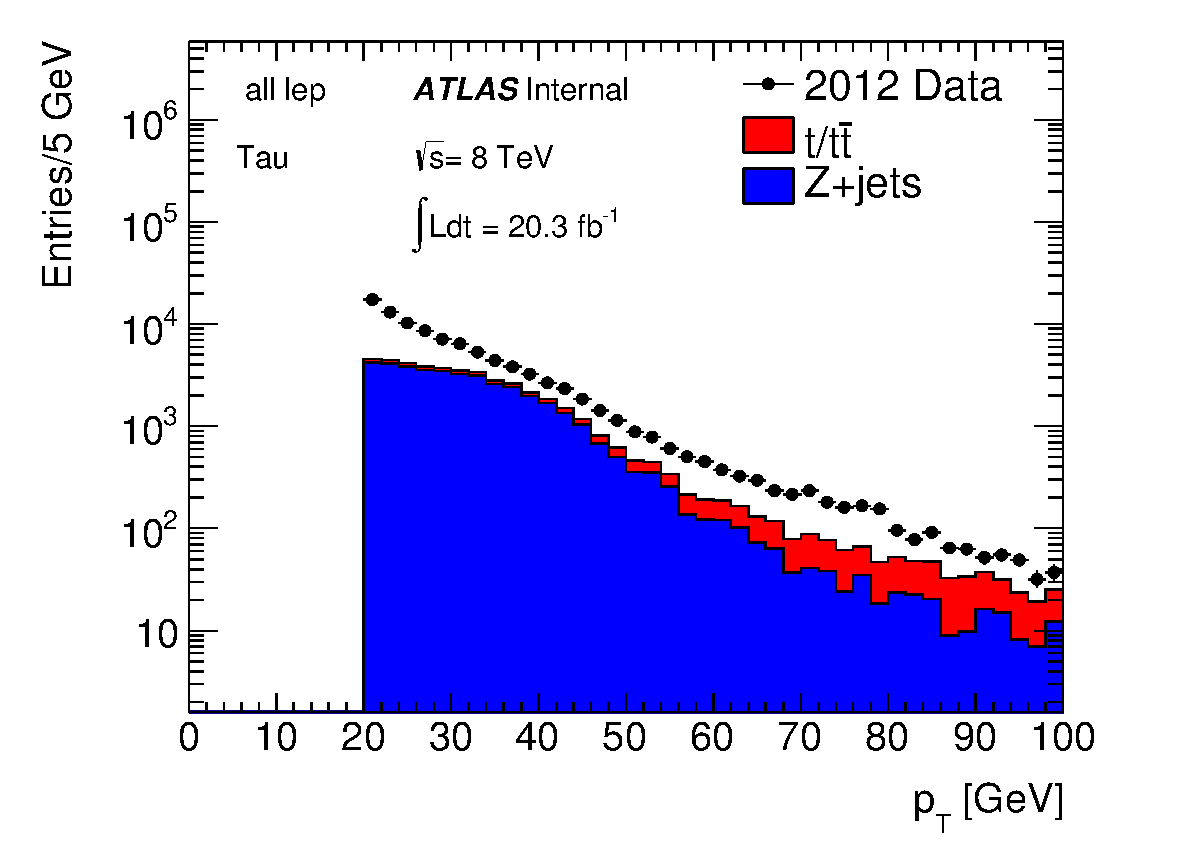
\includegraphics[width=0.48\textwidth]{figures/backgrounds/TauFakes_NumPt}
\centering 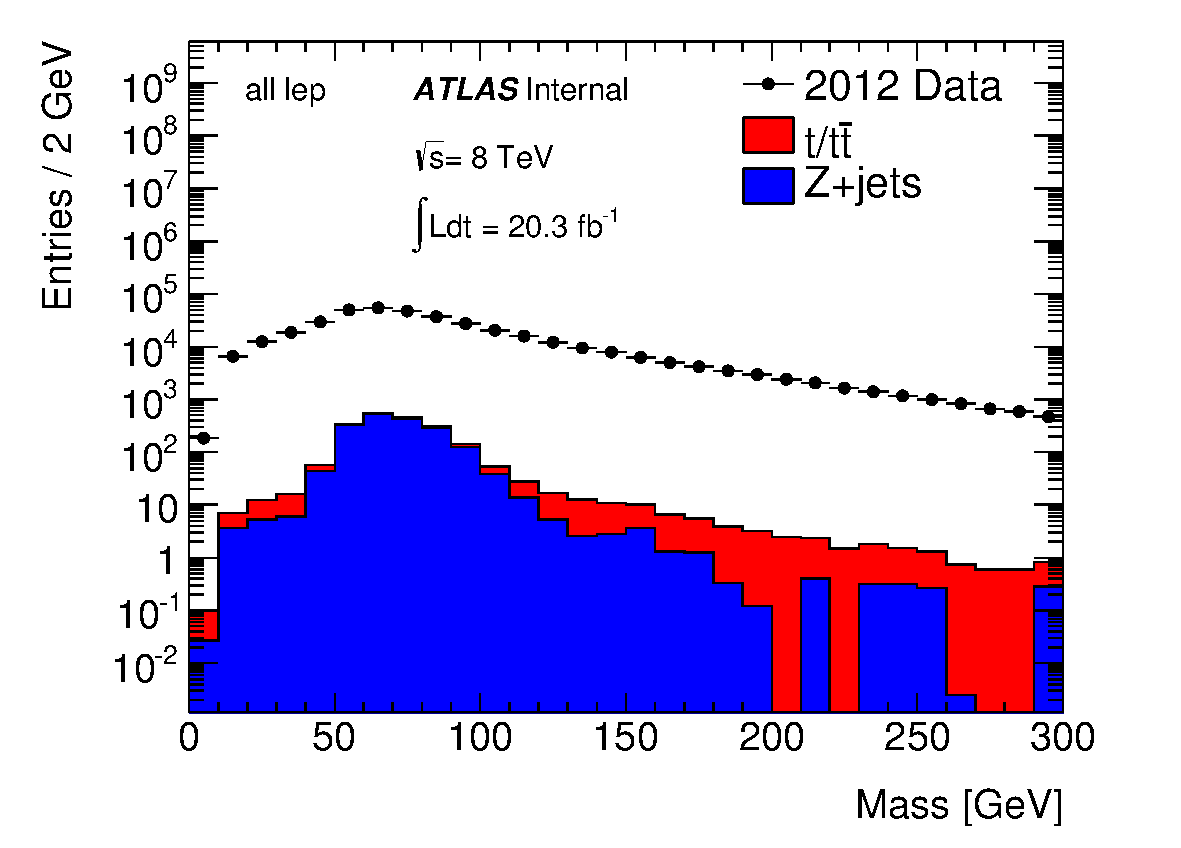
\includegraphics[width=0.48\textwidth]{figures/backgrounds/TauFakes_DenM}
\centering 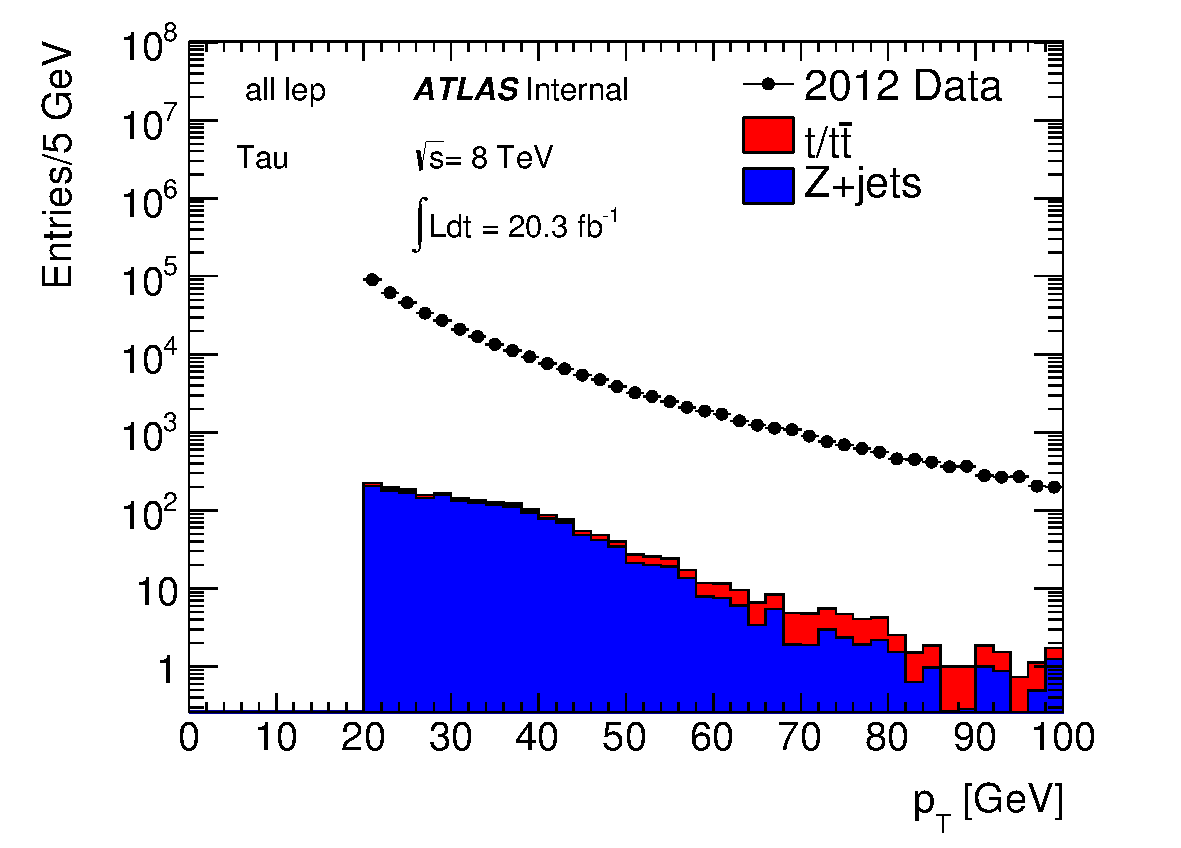
\includegraphics[width=0.48\textwidth]{figures/backgrounds/TauFakes_DenPt}
\caption{\label{fig:taufakeprompt} Invariant mass of the muon and tau pair (left) and
  $p_{T}$ of the tau candidate (right), for the numerator (top) and denominator selections
  (down).  The prompt contribution estimated from MC simulations is shown along with the
  measured data.}
\end{figure}

\begin{figure}
\centering 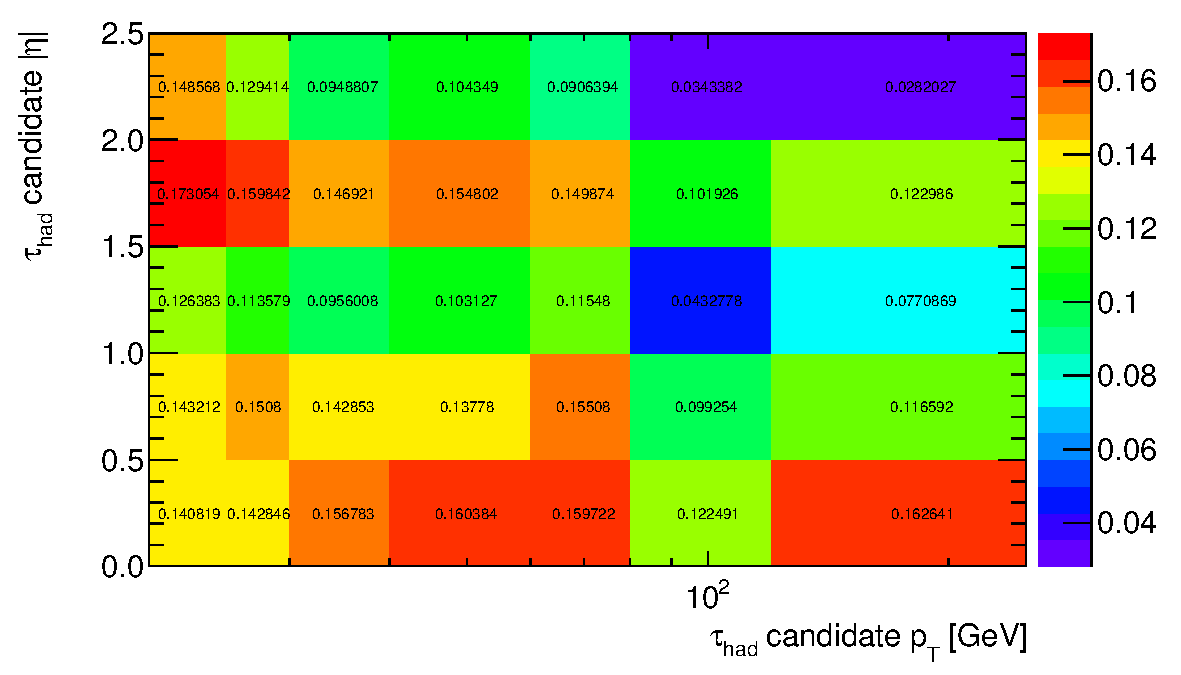
\includegraphics[width=0.48\textwidth]{figures/backgrounds/TauFakes_FFPt}
\centering 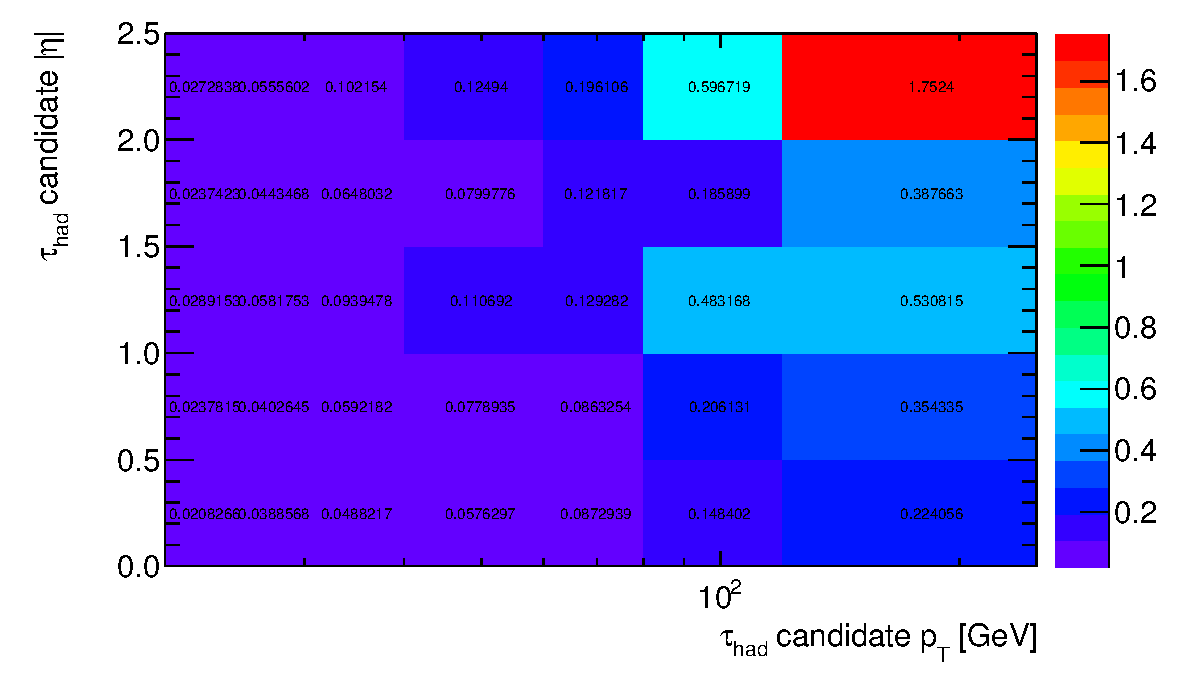
\includegraphics[width=0.48\textwidth]{figures/backgrounds/TauFakes_FFEta}
\centering 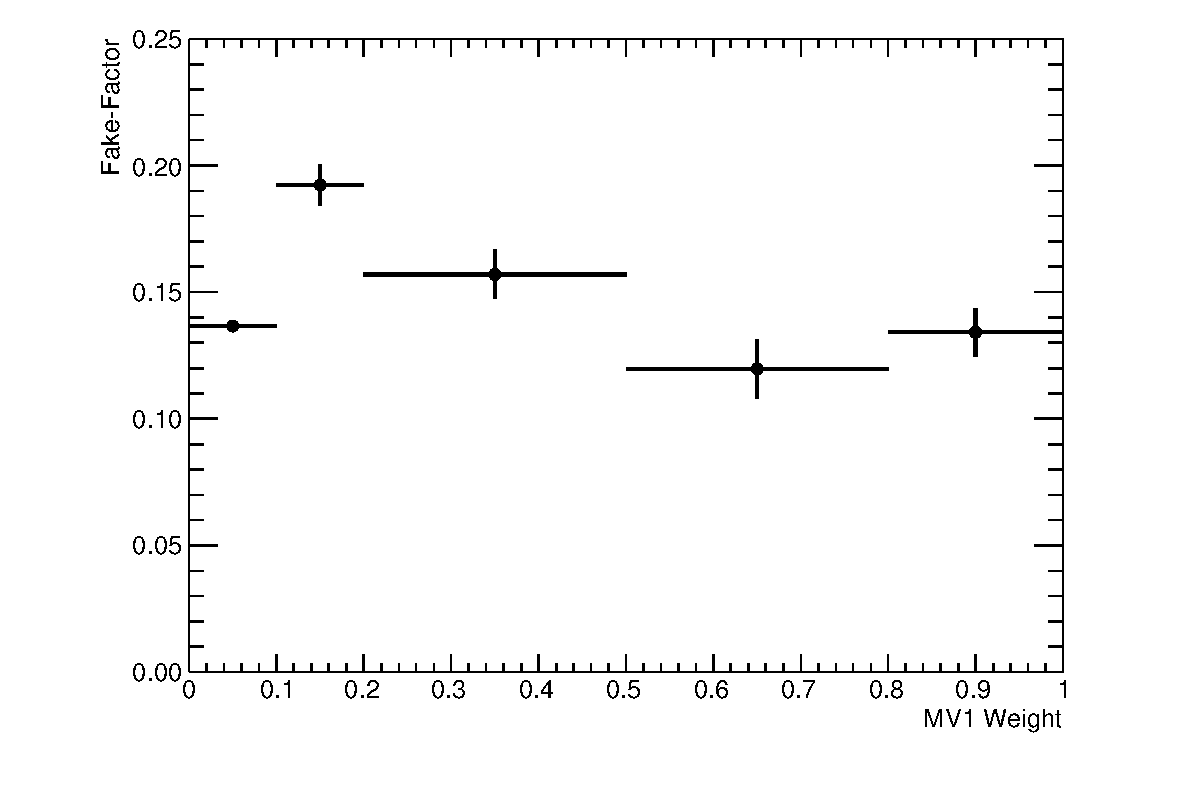
\includegraphics[width=0.48\textwidth]{figures/backgrounds/TauFakes_FFMV1}
\caption{\label{fig:taufakefactors} Fake-factors binned in $p_{T}$ and $|\eta|$ (left) and
  their associated statistical uncertainty (right). The extra scaling as a function of MV1
  weight is also shown (bottom).  These fake-factors were derived in $W$ + jets
  events. The prompt contribution has been subtracted using MC predictions.}
\end{figure}

Figure~\ref{fig:taufakeprompt} shows sample data distributions for the numerator and
denominator tau candidates, along with the prompt contribution which must be subtracted
when calculating the fake-factors. Figure~\ref{fig:taufakefactors} shows the obtained
fake-factors.

\subsection{Systematic Uncertainties}\label{sec:ff-tau-systematics}

Various studies have been carried out to estimate the systematic uncertainties associated
with the tau fake estimates.  The main considered sources of uncertainties are the following:

\begin{itemize}
\item Uncertainties on the MC prompt estimates
\item Uncertainties associated with the binning choice
%\item Dependency of the fake-factors of the $W$ + jets selection
\item Flavour dependence of the fake-factors (gluon, light-quarks, heavy-quarks)
\end{itemize}

For the prompt estimates, the normalization of the MC samples have been fluctuated by
their associated uncertainties (as listed in~\ref{s:syst}).  This results in variations
between 5\% and 17\%, being the largest in the 30-40 GeV $p_{T}$ range (where the prompt
subtraction is the largest due to the $Z$ sample kinematics).

To estimate the effect of the binning on the fake estimates, a closure test is used.  The
fake-factors are re-applied to the same sample they were derived from.  The results of
this test are shown in figure~\ref{fig:tauclosure}.  Excellent agreement is seen, and a
systematic of 5\% is attributed to this effect.

\begin{figure}
\centering 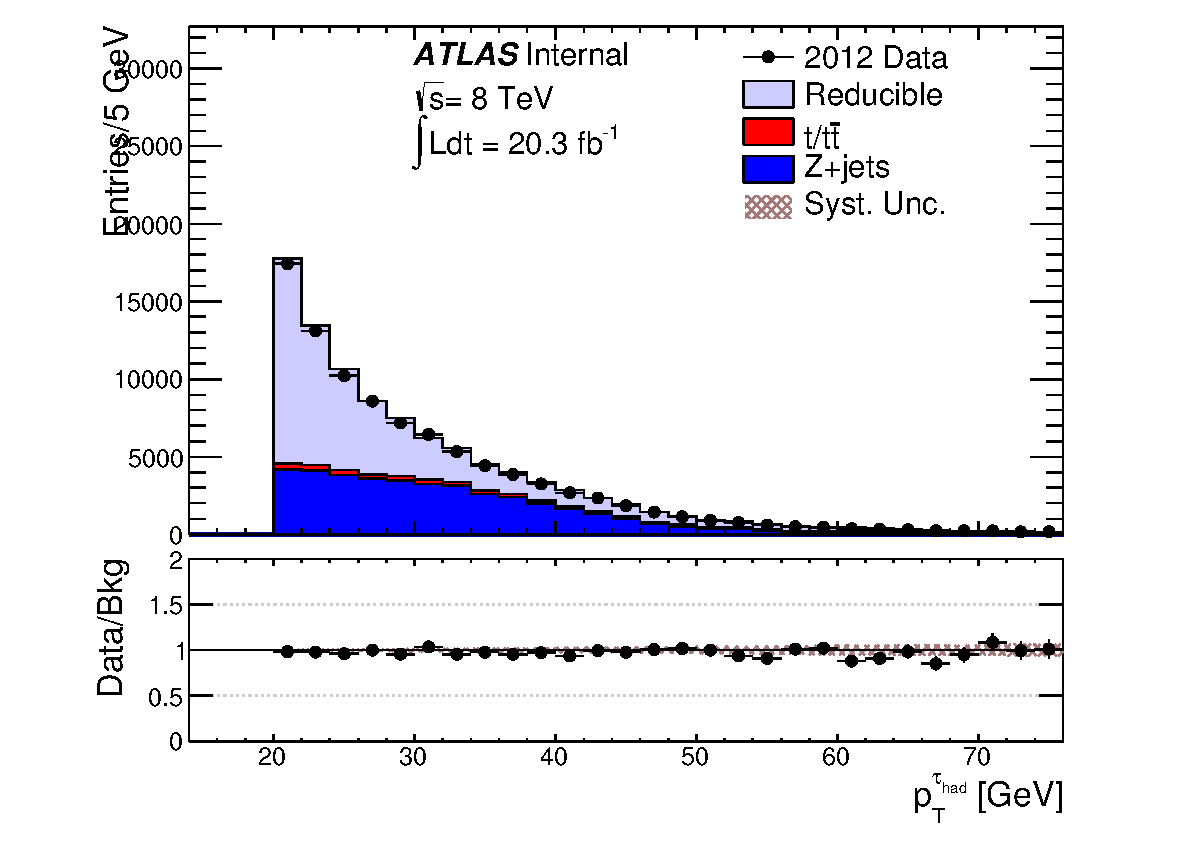
\includegraphics[width=0.48\textwidth]{figures/backgrounds/TauFakes_ClosurePt}
\centering 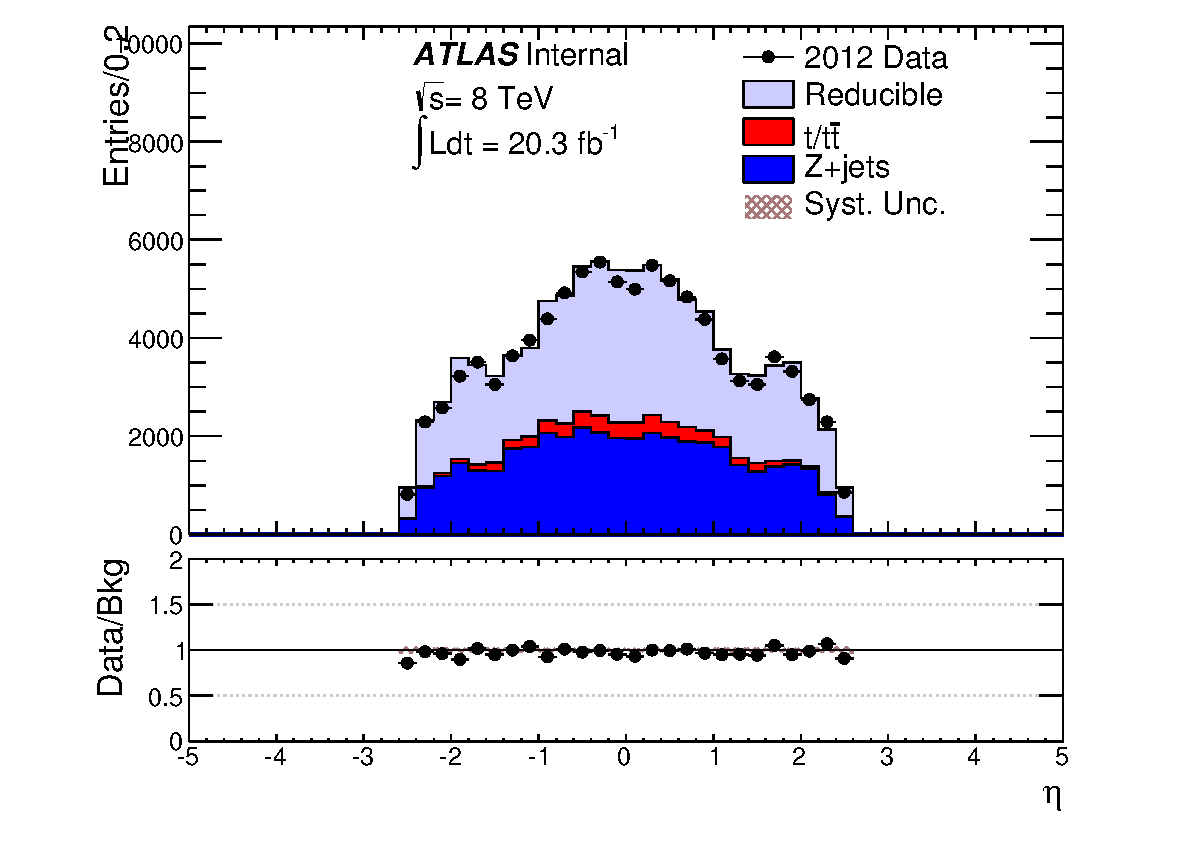
\includegraphics[width=0.48\textwidth]{figures/backgrounds/TauFakes_ClosureEta}
\centering 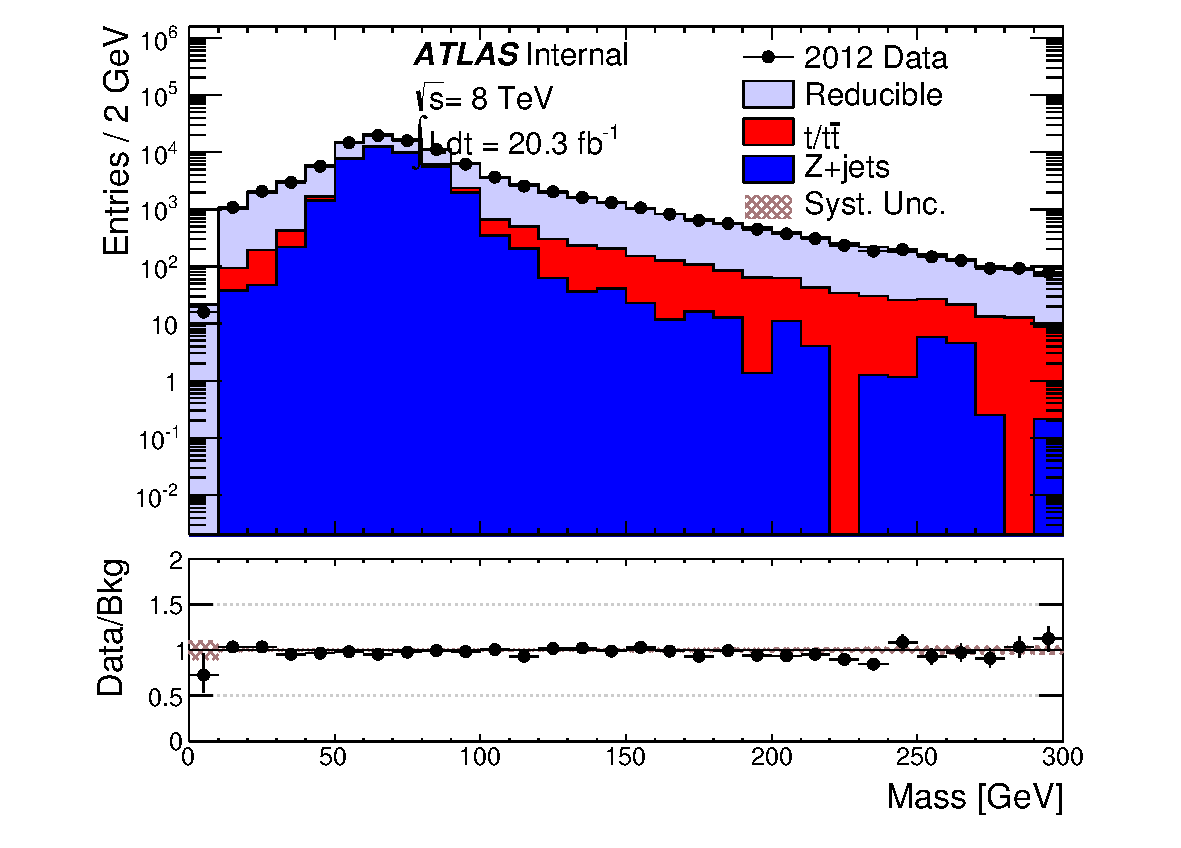
\includegraphics[width=0.48\textwidth]{figures/backgrounds/TauFakes_ClosureMass}
%\centering 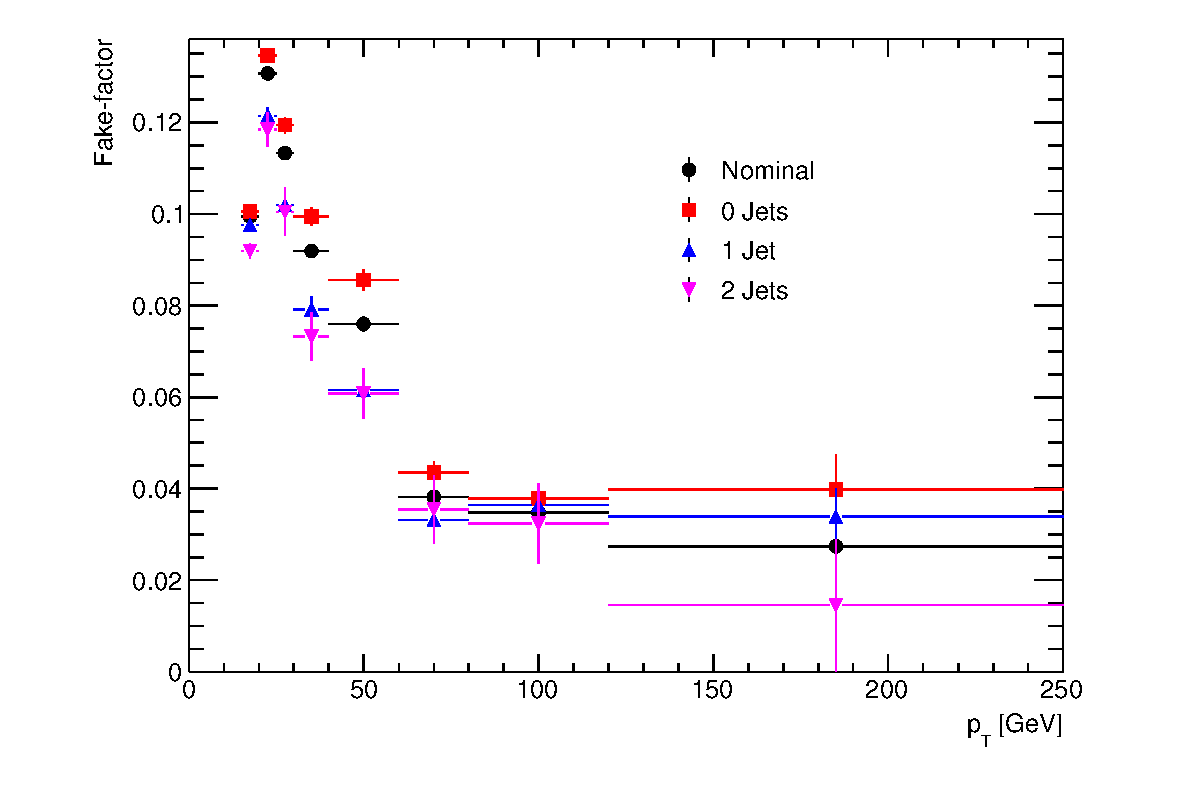
\includegraphics[width=0.48\textwidth]{figures/backgrounds/TauFakes_NJetsDep}
\caption{\label{fig:tauclosure} Distributions of the $\tau$ p$_{T}$ (left), $\tau$ $\eta$
  (right), and invariant mass of the two leptons in the event (bottom).}
\end{figure}

%The uncertainty associated with the assumption that the fake-factors are entirely
%uncorrelated in ($p_{T}$, $\eta$) is evaluated by comparing the fake-factors obtained
%using a 2-D matrix in ($p_{T}$, $\eta$) and the product of the two 1-D fake-factors.  The
%RMS of the distribution is used to estimate the order of this effect, and is approximately
%15\%.

Finally, to estimate the sensitivity of the fake-factors to the flavour composition of the
sample used to derive them, the $t\bar{t}$ validation region described in~\ref{s:CR_Top}
is used. This sample was found in MC studies to have a largely different flavour
composition than the nominal $W$ + jets sample, and can therefore be used to put a
conservative systematic on this effect.  A flat variation of 25\% is found to bracket this
effect conservatively across all observables.

As a cross-check, the same effect can be probed less directly by tuning the requirements
of the $W$ + jets sample. The selection requirements applied to the $W$ + jets sample will
directly affect the kinematics and flavour composition of the sample, and lead to
differences in the derived fake-factors. While there is no direct way to measure how
different the compositions are between the $W$ + jets control sample and the signal
regions, it is possible to approximate how sensitive the fake-factors are to such changes.
Some selection requirements aimed at rejecting $Z$ + jets events are applied to derive
different sets of fake-factors, inspired by~\cite{zttnote,tauidnote}.  The following
requirements are applied separately:

\begin{itemize}
\item $\cos{\Delta\phi(\mu, \met)} + \cos{\Delta\phi(\tau, \met)} <$ -0.15
\item $m_{T}^{\mu} >$ 70 GeV
\item $m_{Z}^{vis.} <$ 42 GeV or $m_{Z}^{vis.} >$ 82 GeV
\item $p_{T}^{\mu} >$ 35 GeV
\end{itemize}

\begin{figure}
\centering 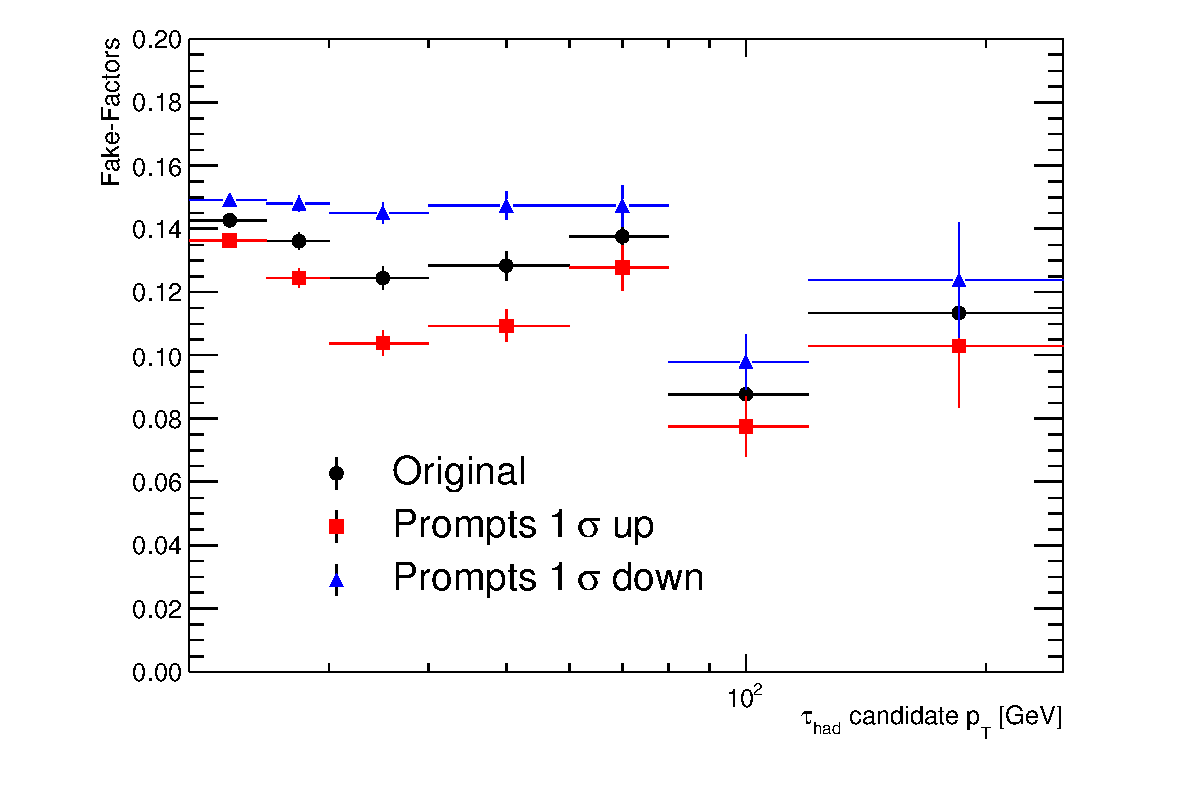
\includegraphics[width=0.48\textwidth]{figures/backgrounds/TauFakes_PromptsDep}
\centering 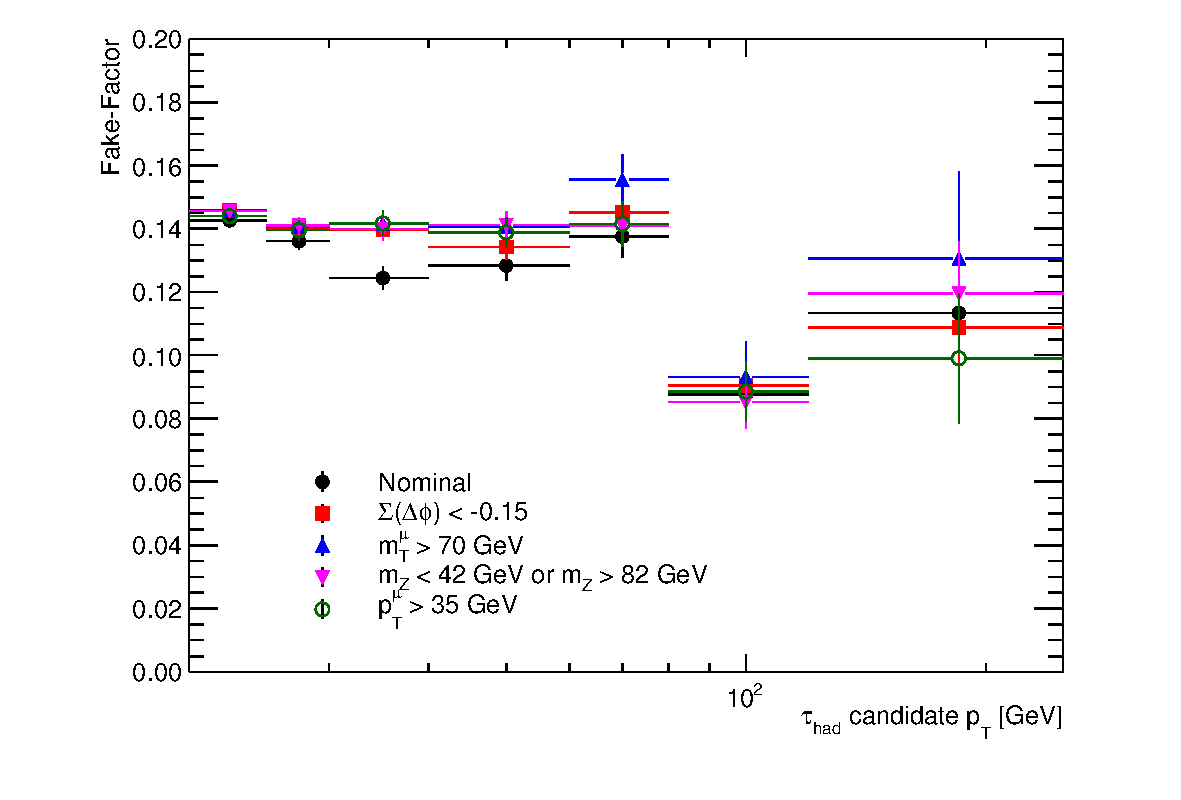
\includegraphics[width=0.48\textwidth]{figures/backgrounds/TauFakes_CutsDep}
%\centering 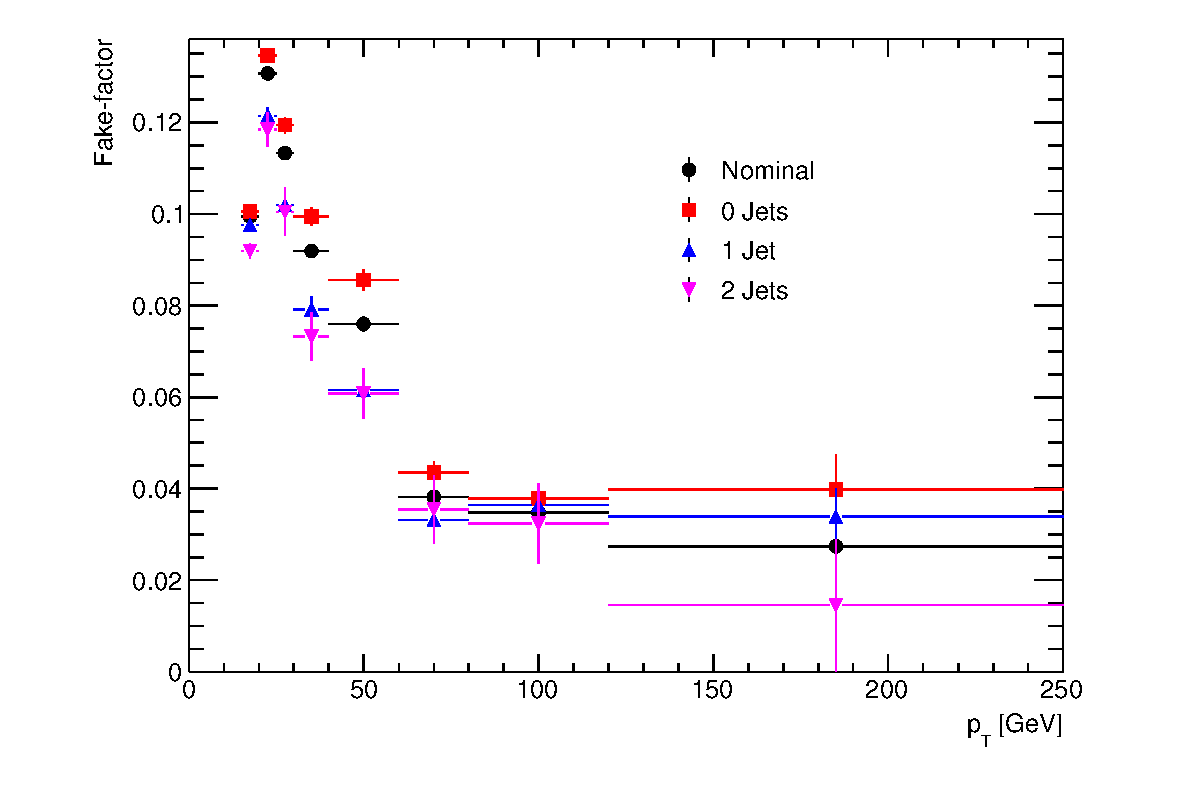
\includegraphics[width=0.48\textwidth]{figures/backgrounds/TauFakes_NJetsDep}
\caption{\label{fig:fakesys} Dependency of the fake-factors on the prompt normalization
  (left) and the $W$ event requirements based on the cuts to reject $Z$ events (right).}
\end{figure}

The resulting sets of fake-factors are shown in figure~\ref{fig:fakesys}.  The variations
are no larger than 12\%, and are therefore bracketed by the 25\% estimate from the
$t\bar{t}$ sample.

In the end, the systematics are found to vary between 25\% and 30\%, being largest where
the prompt subtraction is most significant.


% Alternatively,
%making different requirements on the number of jets produced in association with the $W$
%leads to variations in the flavour composition of the sample. Fake-factors derived with
%different requirements on the number of jets are also shown in figure~\ref{fig:fakesys}.
%The scale of these variations due to different selection requirements on the $W$ + jets
%events is typically in the order of 20\% or less.


%Ultimately, a more direct way to probe how well the fake-factors model the reducible
%backgrounds consists in studying validation regions.  Three different validations regions are
%used, aimed at probing prompt and fake taus in $Z$-like and $t\bar{t}$ dilepton events,
%and in trilepton events where a $Z$ boson is well-reconstructed.  These 3 validation
%regions probe different topologies, and would reveal any mismodeling associated with this
%method.  Using the good degree of agreement found in the validation, and the magnitude of
%the effects studied above, a conservative flat uncertainty of 25\% is used for all $\tau$
%fake estimates.


% This is what you previously had in the resonance chapter. Probably redundant, but it does have fine details about the MC samples.
%\section{Background Estimation}
%The backgrounds to the trilepton resonance search are similar to those for the model-independent search described in section~\ref{sec:background-estimation}. In the \fourl signal regions, $ZZ$ production is dominant. In the $\threeljj$ and $\threelo$ signal regions, $WZ$ production is dominant, with smaller contributions from $ZZ$ where one lepton is not selected, $\ttbarV$, and reducible backgrounds. 
%
%The prompt backgrounds are estimated using Monte Carlo simulation. The samples are detailed below in section~\ref{sec:resonance-background-MC-samples}. The reducible $Z+\gamma$ backgrounds are also estimated using simulation. The remaining reducible backgrounds are estimated using the same fake factor method as described in section~\ref{sec:fake-factor-method}. 
%
%\subsection{Background Monte Carlo Samples}\label{sec:resonance-background-MC-samples}
%
%\begin{table}
%  \centering
%  \caption{Summary of the \textcolor{black}{primary} signal and background MC samples used in this analysis. The generator, parton shower and hadronization, PDF, underlying event tune, and the order of the cross-section calculation are shown for each sample.}
%  \begin{tabular}{|c|c|c|c|c|c|}
%    \hline
%    Process & Generator & Parton shower and hadr. & PDF set & UE tune & Cross section \\
%    \hline
%    VLL & \madgraph\ 4.5.2 & \pythia\ 8 & CTEQ6L1 & AU2	&	LO 	\\
%    Seesaw & \madgraph\ 5.2.2.1 & \pythia\ 8 & CTEQ6L1 & AU2	&	LO 	\\
%    $WZ$ & \sherpa 1.4.3 & \sherpa & CT10 & \sherpa 	&	NLO\\
%    $ZZ$ & \sherpa 1.4.5 & \sherpa & CT10 & \sherpa 	&	NLO\\
%   % $\ttbar+W/Z$ & \alpgen\ 2.13 ~\cite{alpgen}  & \herwig\ 6.520~\cite{herwig}   & CTEQ6L1 & \jimmy\ 4.31~\cite{jimmy} 	&	\\
%    $\ttbar+W/Z$ & \madgraph\ 5.1.3.33  & \pythia\ 6.426   & {CTEQ6L1} & AUET2B 	&	NLO\\
%    $VVV^{(*)}$ & \madgraph\ 5.1.3.33 & \pythia\ 6.426 & {CTEQ6L1}  & AUET2B 	& 	LO	\\
%    $Z+\gamma$ & \sherpa  & \sherpa & CT10 & \sherpa 	&	LO 	\\
%    \hline
%  \end{tabular}
%  \label{table:resonance-background-samples}
%\end{table}
%
%
%The Monte Carlo samples used to model the background processes are summarized in table~\ref{table:resonance-background-samples}. For all samples, the response of the ATLAS detector is modelled using the \geant~toolkit~\cite{geant,atlassimulation}. Pileup interactions in the same or nearby bunch crossings are modeled by overlaying minimum-bias interactions modelled with \pythia~6.425 onto the hard-scatter event. The simulated events are assigned weights to reprocude the distribution of the average number of $pp$ interactions per crossing observed in data. 
%
%The dominant backgrounds due to Standard Model $WZ$ ($ZZ$) production are modelled using the \sherpa~\cite{sherpa} MC generator version 1.4.3 (1.4.5), using the internal showering algorithm~\cite{Hoeche:2009rj,Gleisberg:2008fv,Schumann:2007mg}a nd  the CT10~\cite{ct10} PDF set. The samples are normalized using cross sections calculated at next-to-leading-order (NLO) in QCD with \vbfnlo-2.6.2~\cite{vbfnlo}.  The generation includes up to three additional parton emissions in the matrix element. Samples of simulated events based on the NLO generator \powheg~\cite{powheg} are used to derive systematic uncertainties on the shapes of distributions predicted by \sherpa. The diboson samples are showered with \pythia~8, and use the CT10 PDF set and AU2 underlying event tune.
%
%Drell--Yan production in association with a photon that converts in the detector, denoted $Z+\gamma$, is modelled using \sherpa~1.4.1, also using the CT10 PDF set and including up to three additional parton emissions in the matrix element. Production of top-quark pairs in association with a $W$ or $Z$ boson ($\ttbarV$) and triboson production ($VVV^{(*)}$) are modelled using \madgraph~5.1.3.33, with \pythia~6.426 for the parton shower and hadronization, AUET2B underlying event tune~\cite{AUET2B}, and the CTEQ6L1 PDF set. The $\ttbarV$ processes are normalized to the corresponding NLO cross sections~\cite{Campbell:2012dh,Lazopoulos:2008de}, while the $Z+\gamma$ and $VVV^{(*)}$ processes are normalized to their LO cross sections from the respective generator.

\section{Application of Fake Factors}\label{sec:fake-factor-application}
Figure~\ref{fig:prompt-subtractions} shows the fake factor-weighted reducible events in the signal regions, as given by equation~\ref{eq:fake-factor-master-formula}. The estimated prompt subtractions due to $Z+\gamma$, $WZ$, $ZZ$, $t\overline{t}+V$, and $VVV^{(*)}$ events (i.e. the contributions to events with denominator objects due these irreducible background sources, rather than the intended sources of reducible background) are shown in the colored histograms. The reducible background prediction is the difference between the data points and the prompt subtraction histograms. In cases where a bin is negative after applying the prompt subtraction, the contents of that bin are set to zero, and the histogram is scaled to preserve the overall normalization. 
%For the 4L, $Z+e$ signal region, the overall normalization is negative and consistent with zero, so the background is neglected in this region. 

The uncertainty on the background prediction is the combination of two components: the systematic uncertainties on the electron and muon fake factors, and the statistical uncertainties due to finite events with denominator objects. As described in section~\ref{sec:systematic-uncertainties}, the fake factor uncertainties constitute their own component, while the statistical uncertainties are contained in the ``Monte Carlo statistics'' component. 

\begin{figure}[h]
	\centering
	\subfloat[ Inclusive SR, $Z+e$] {
		\resizebox{3in}{!}{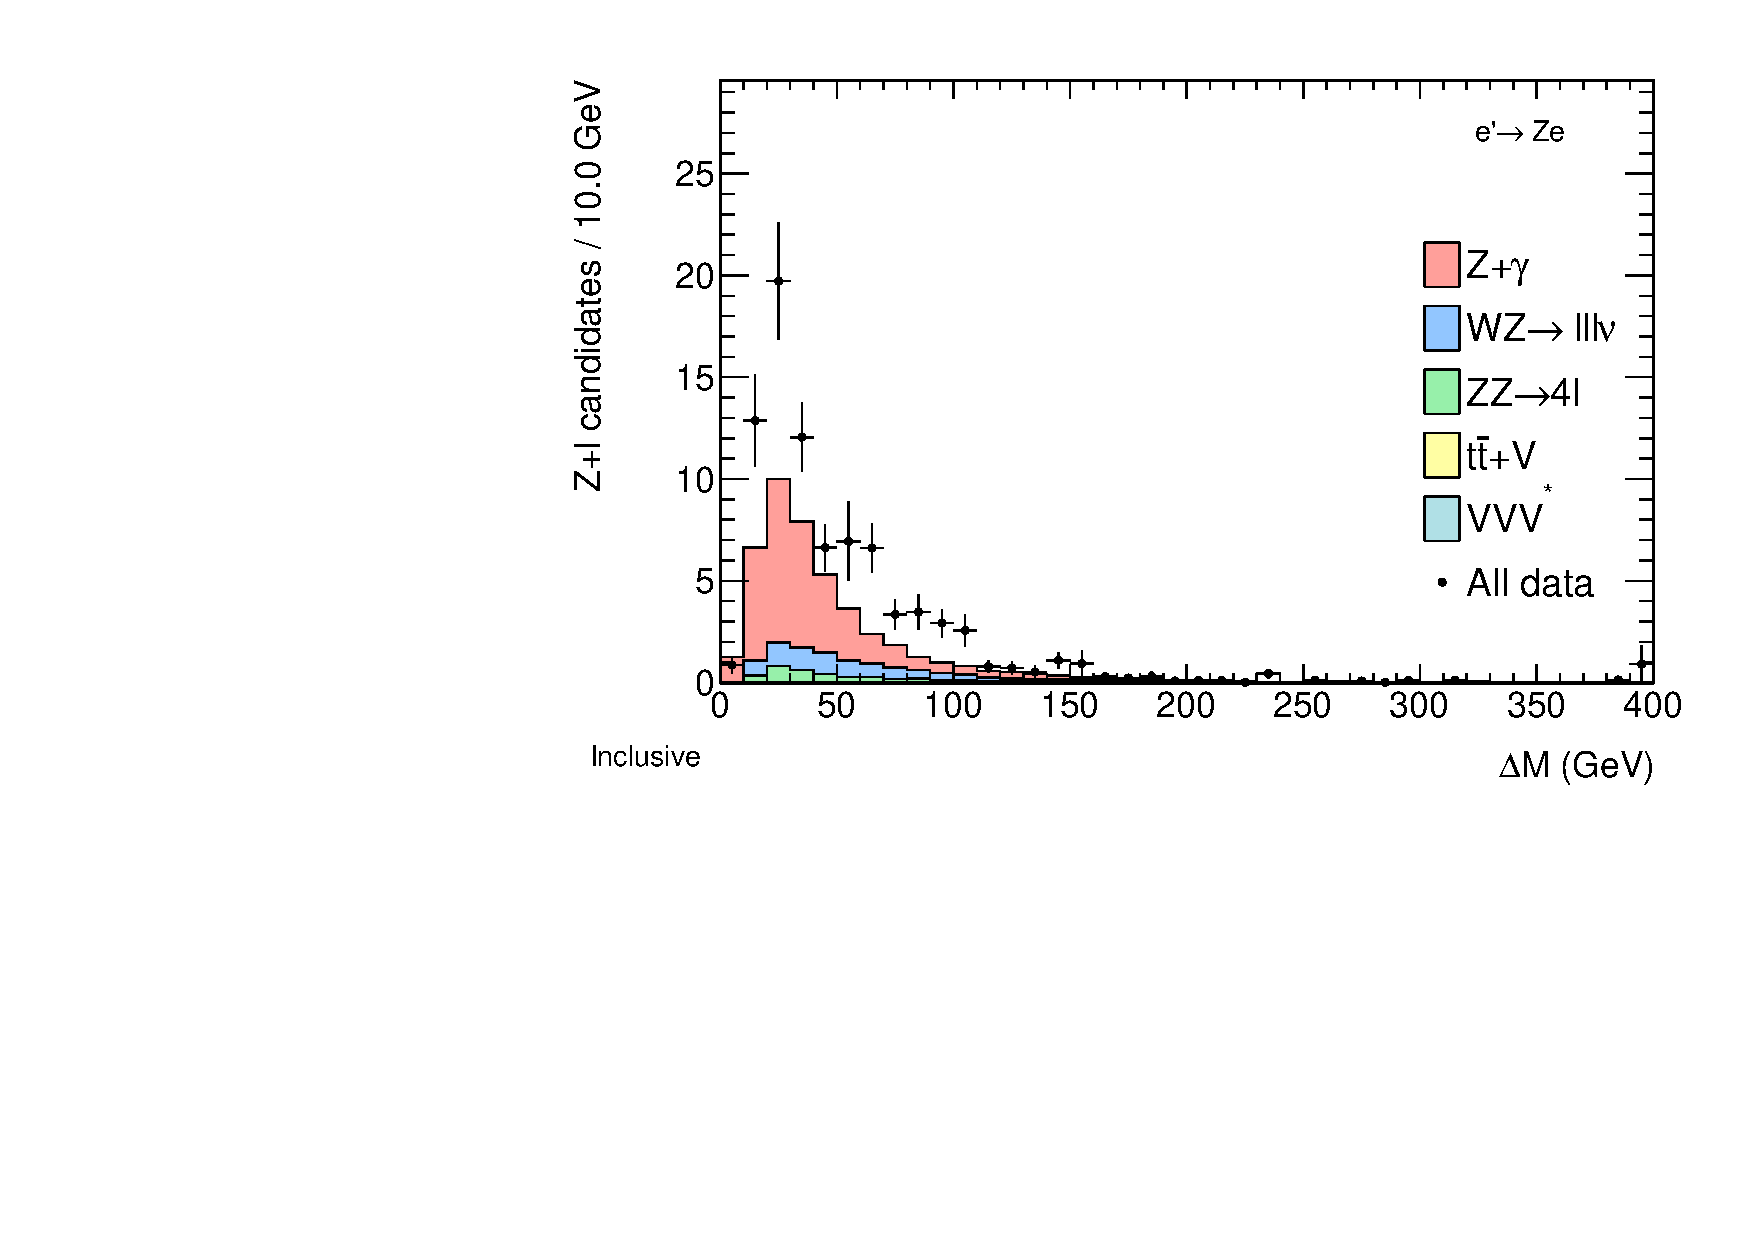
\includegraphics{figures/backgrounds/c_output_reducible_DeltaM_Ze_InclusiveNoM3L}}
	}
	\subfloat[ Inclusive SR, $Z+\mu$] {
		\resizebox{3in}{!}{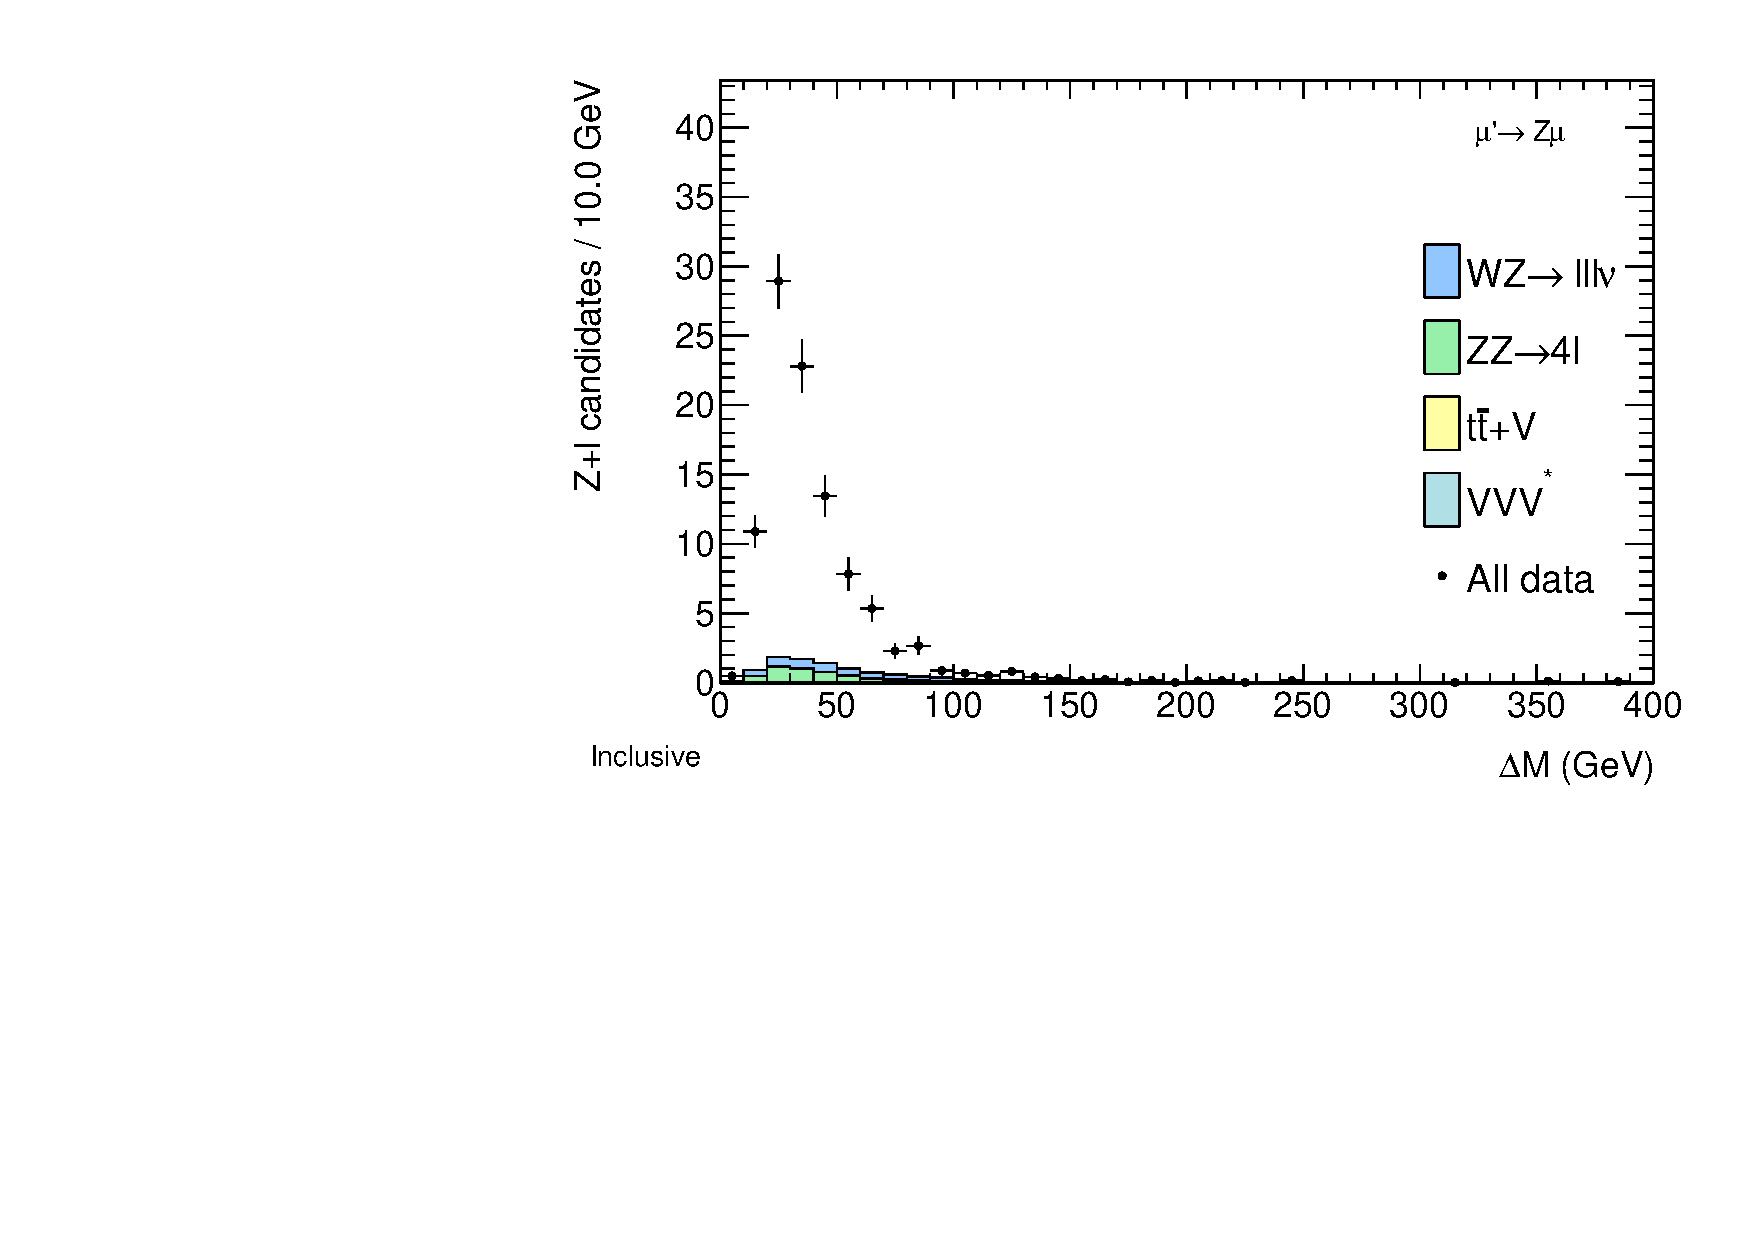
\includegraphics{figures/backgrounds/c_output_reducible_DeltaM_Zmu_InclusiveNoM3L}}
	} \\
	\subfloat[ 4L SR, $Z+e$] {
		\resizebox{3in}{!}{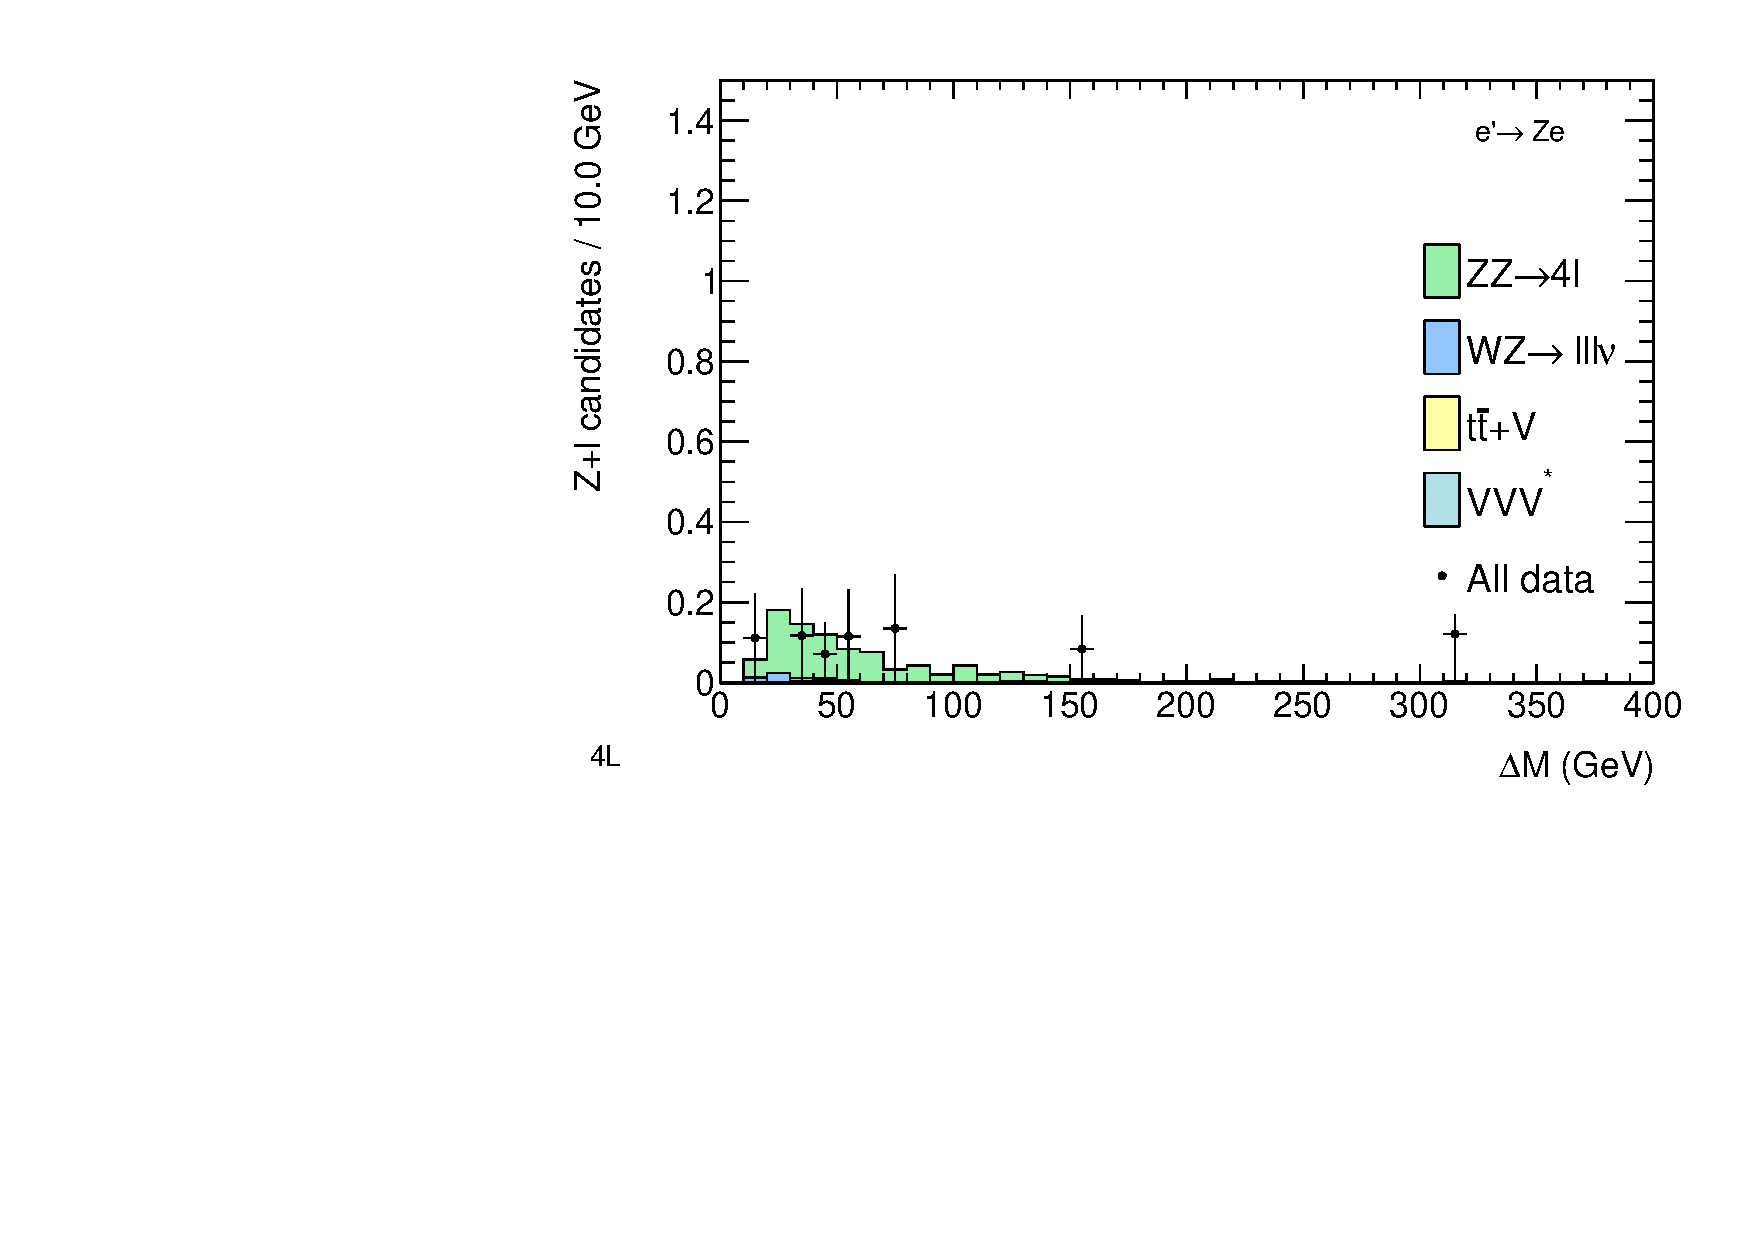
\includegraphics{figures/backgrounds/c_output_reducible_DeltaM_Ze_FourLNoM3L}}
	}
	\subfloat[ 4L SR, $Z+\mu$] {
		\resizebox{3in}{!}{\includegraphics{figures/backgrounds/c_output_reducible_DeltaM_Zmu_FourLNoM3L}}
	} \\
	\subfloat[ 3L+dijet SR, $Z+e$] {
		\resizebox{3in}{!}{\includegraphics{figures/backgrounds/c_output_reducible_DeltaM_Ze_ThreeLDijetNoM3L}}
	}
	\subfloat[ 3L+dijet SR, $Z+\mu$] {
		\resizebox{3in}{!}{\includegraphics{figures/backgrounds/c_output_reducible_DeltaM_Zmu_ThreeLDijetNoM3L}}
	} \\
	\caption{Fake factor-weighted data events and prompt subtractions. The reducible background prediction is the difference between the data points and the prompt subtraction colored histograms.}
	\label{fig:prompt-subtractions}
\end{figure}
